\documentclass[12pt]{article}
\usepackage{indentfirst}
\usepackage{graphicx}
\usepackage[margin=1.3in, top=1.4in]{geometry}
\usepackage[section]{placeins}
\usepackage{booktabs}
\usepackage{tabularx} 
\usepackage{tabulary}
\usepackage{cutwin}
\usepackage{caption}
\usepackage{lipsum}
\usepackage{wrapfig}
\usepackage[T1]{fontenc}
\usepackage{color}
\usepackage{eurosym}
\usepackage{glossaries}
\usepackage{subcaption}
\usepackage{amsmath}
\usepackage[utf8x]{inputenc}
\usepackage{url}
\usepackage[hidelinks]{hyperref}
\usepackage{float}
\usepackage[table,xcdraw]{xcolor}
\usepackage{dirtree}
\usepackage[title,titletoc,toc]{appendix}

\usepackage[justification=centering]{caption}


\usepackage{listings}
\usepackage{color}
\definecolor{mygreen}{rgb}{0,0.6,0}
\definecolor{mygray}{rgb}{0.5,0.5,0.5}
\definecolor{mymauve}{rgb}{0.58,0,0.82}


%%%TAB COMAND
\newcommand\tab[1][1cm]{\hspace*{#1}}


%%%%%%%%%%%%%%%%%%%%%%%%%%%%%%%%%%
%subsubsubsection
\usepackage{titlesec}
%\usepackage{hyperref}
\titleclass{\subsubsubsection}{straight}[\subsection]
\newcounter{subsubsubsection}[subsubsection]
\renewcommand\thesubsubsubsection{\thesubsubsection.\arabic{subsubsubsection}}
\renewcommand\theparagraph{\thesubsubsubsection.\arabic{paragraph}} % optional; useful if paragraphs are to be numbered
\titleformat{\subsubsubsection}
  {\normalfont\normalsize\bfseries}{\thesubsubsubsection}{1em}{}
\titlespacing*{\subsubsubsection}
{0pt}{3.25ex plus 1ex minus .2ex}{1.5ex plus .2ex}
\makeatletter
\renewcommand\paragraph{\@startsection{paragraph}{5}{\z@}%
  {3.25ex \@plus1ex \@minus.2ex}%
  {-1em}%
  {\normalfont\normalsize\bfseries}}
\renewcommand\subparagraph{\@startsection{subparagraph}{6}{\parindent}%
  {3.25ex \@plus1ex \@minus .2ex}%
  {-1em}%
  {\normalfont\normalsize\bfseries}}
\def\toclevel@subsubsubsection{4}
\def\toclevel@paragraph{5}
\def\toclevel@paragraph{6}
\def\l@subsubsubsection{\@dottedtocline{4}{7em}{4em}}
\def\l@paragraph{\@dottedtocline{5}{10em}{5em}}
\def\l@subparagraph{\@dottedtocline{6}{14em}{6em}}
\makeatother
\setcounter{secnumdepth}{4}
\setcounter{tocdepth}{4}
%%%%%%%%%%%%%%%%%%%%%%%%%%%%%%%%%%%%%%%%%%%%%%%

\sloppy

 \definecolor{mygreen}{rgb}{0,0.6,0}
\definecolor{mygray}{rgb}{0.5,0.5,0.5}
\definecolor{mymauve}{rgb}{0.58,0,0.82}

% Define Language
\lstdefinelanguage{EL}
{
% list of keywords
morekeywords={language,
interface,
service,
services,
reference,
references,
properties,
int,
float,
string,
bool,
subcomponents,
component,
bind,
to,
promote,
as,
import,
compile },
sensitive=false, % keywords are not case-sensitive
morecomment=[l]{//}, % l is for line comment
morecomment=[s]{/*}{*/}, % s is for start and end delimiter
morestring=[b]" % defines that strings are enclosed in double quotes
}

% Set Language
\lstset{
%language={EL},
aboveskip=2\bigskipamount,
backgroundcolor=\color{white}, % choose the background color; you must add \usepackage{color} or \usepackage{xcolor}
basicstyle=\scriptsize, % the size of the fonts that are used for the code
breakatwhitespace=false, % sets if automatic breaks should only happen at whitespace
breaklines=true, % sets automatic line breaking
captionpos=b, % sets the caption-position to bottom
commentstyle=\color{mygreen}, % comment style
deletekeywords={...}, % if you want to delete keywords from the given language
escapeinside={\%*}{*)}, % if you want to add LaTeX within your code
extendedchars=true, % lets you use non-ASCII characters; for 8-bits encodings only, does not work with UTF-8
frame=lines, % adds a frame around the code
keepspaces=true, % keeps spaces in text, useful for keeping indentation of code (possibly needs columns=flexible)
keywordstyle=\color{blue}, % keyword style
% otherkeywords={*,language, interface,
% service, services, reference, references, properties, int, float, string, bool, subcomponents, component, bind, to, promote, as,import,compile, ...}, % if you want to add more keywords to the set
numbers=none, % where to put the line-numbers; possible values are (none, left, right)
numbersep=5pt, % how far the line-numbers are from the code
numberstyle=\tiny\color{mygray}, % the style that is used for the line-numbers
rulecolor=\color{black}, % if not set, the frame-color may be changed on line-breaks within not-black text (e.g. comments (green here))
showspaces=false, % show spaces everywhere adding particular underscores; it overrides 'showstringspaces'
showstringspaces=false, % underline spaces within strings only
showtabs=false, % show tabs within strings adding particular underscores
stepnumber=2, % the step between two line-numbers. If it's 1, each line will be numbered
stringstyle=\color{mymauve}, % string literal style
tabsize=2, % sets default tabsize to 2 spaces
title=\lstname, % show the filename of files included with \lstinputlisting; also try caption instead of title
%xleftmargin=20.0pt,
%xrightmargin=20.0pt
}


%space between paragraphs
\setlength{\parskip}{0.8ex}

\begin{document}

\begin{titlepage}

\newcommand{\HRule}{\rule{\linewidth}{0.5mm}} % Defines a new command for the horizontal lines, change thickness here

\center % Center everything on the page
 
%----------------------------------------------------------------------------------------
%	HEADING SECTIONS
%----------------------------------------------------------------------------------------

\textsc{\LARGE FINAL REPORT}\\[1.0cm] % Major heading such as course name
\textsc{\Large Project II}\\[0.5cm] % Minor heading such as course title
\textsc{\large Embedded Systems Research Group}\\[0.5cm] % Minor heading such as course title

%----------------------------------------------------------------------------------------
%	TITLE SECTION
%----------------------------------------------------------------------------------------

\HRule \\[1.2cm]
{ \Huge \bfseries 
Modeling a Dynamic Binary Translator using a DSL}\\[1.0cm] % Title of your document 
{ \Large \bfseries 
Decoding Operands}\\[0.4cm]

\HRule \\[2.0cm]
 
%----------------------------------------------------------------------------------------
%	AUTHOR SECTION
%----------------------------------------------------------------------------------------
% Your name
\begin{minipage}{0.4\textwidth}
\begin{flushleft} \large
\emph{Authors:}\\
Ana Rita \textsc{Martins} 64743 \\
David \textsc{Almeida} 68532 \\
Nelson \textsc{Pinto} 68586 \\
Paulo \textsc{Félix} 61767  \\
Pedro \textsc{Guimarães} 68539 \\
Pedro \textsc{Pereira} 68525 \\
Ricardo \textsc{Teixeira} 68562

\end{flushleft}
\end{minipage}
~
\begin{minipage}{0.4\textwidth}
\begin{flushright} \large
 \emph{Advisors:} \\
Filipe \textsc{Salgado} \\ % Supervisor's Name
\end{flushright}
\end{minipage}\\[2cm]

%----------------------------------------------------------------------------------------
%	LOGO SECTION
%----------------------------------------------------------------------------------------
%\includegraphics{Logo}\\[1cm] % Include a department/university logo - this will require the graphicx package
%----------------------------------------------------------------------------------------
\noindent\begin{minipage}{0.2\textwidth}

\includegraphics[width=\linewidth]{images/logo} \\[0.5cm] 
\end{minipage}%
\hfill%

{ \large \bfseries 
Universidade do Minho}\\[0.5cm] 

%----------------------------------------------------------------------------------------
%	DATE SECTION
%----------------------------------------------------------------------------------------
{\large \today}\\[3cm] % Date, change the \today to a set date if you want to be precise

\vfill % Fill the rest of the page with whitespace
\end{titlepage}


\begin{abstract}
The use of Domain Specific Languages (DSL) can result in high productivity and high quality design in the generation of final configurable projects. The current project covers the process of modeling an embedded system, more specifically a Dynamic Binary Translator, through the use of a new DSL called EL language, in order to obtain a configurable system. 

The work done results in the design of a conceptual model and a implementation that validates the use of these tools. The model created was based on a Service Component Architecture (SCA) that allows the definitions of computational entities described as components. Components can be arrange into composites and linked through services and references. This allows to describe complex architecture composed by replaceable modules.  

Using a modeling framework, the \textit{EL} framework, it was possible to create a representation of the model in code and from there achieve a goal where it is possible to configure some particular parameters of the system and generate final source files of a Dynamic Binary Translator. 

\newpage
\end{abstract}

%%%%%%%%%%%%%%%%%%%%%%%%%%%%%%%%%%%%%%%%%%%%%%%%%%%%%%%%%%%%%%%%%%%%%%%%%%%%%%%%%%
% Table of Contents
%%%%%%%%%%%%%%%%%%%%%%%%%%%%%%%%%%%%%%%%%%%%%%%%%%%%%%%%%%%%%%%%%%%%%%%%%%%%%%%%%%
\renewcommand{\listfigurename}{Contents}
%\newpage
\tableofcontents

%%%%%%%%%%%%%%%%%%%%%%%%%%%%%%%%%%%%%%%%%%%%%%%%%%%%%%%%%%%%%%%%%%%%%%%%%%%%%%%%%%
% Table of Figures
%%%%%%%%%%%%%%%%%%%%%%%%%%%%%%%%%%%%%%%%%%%%%%%%%%%%%%%%%%%%%%%%%%%%%%%%%%%%%%%%%%
\renewcommand{\listfigurename}{Figures}
%\newpage
\listoffigures

%%%%%%%%%%%%%%%%%%%%%%%%%%%%%%%%%%%%%%%%%%%%%%%%%%%%%%%%%%%%%%%%%%%%%%%%%%%%%%%%%%
% Table of Tables
%%%%%%%%%%%%%%%%%%%%%%%%%%%%%%%%%%%%%%%%%%%%%%%%%%%%%%%%%%%%%%%%%%%%%%%%%%%%%%%%%%
\renewcommand{\listtablename}{Tables}
%\newpage
\listoftables

%%%%%%%%%%%%%%%%%%%%%%%%%%%%%%%%%%%%%%%%%%%%%%%%%%%%%%%%%%%%%%%%%%%%%%%%%%%%%%%%%%
% Table of Listings
%%%%%%%%%%%%%%%%%%%%%%%%%%%%%%%%%%%%%%%%%%%%%%%%%%%%%%%%%%%%%%%%%%%%%%%%%%%%%%%%%%

%\newpage
\lstlistoflistings

%%%%%%%%%%%%%%%%%%%%%%%%%%%%%%%%%%%%%%%%%%%%%%%%%%%%%%%%%%%%%%%%%%%%%%%%%%%%%%%%%%
% Glossaries
%%%%%%%%%%%%%%%%%%%%%%%%%%%%%%%%%%%%%%%%%%%%%%%%%%%%%%%%%%%%%%%%%%%%%%%%%%%%%%%%%%
\newglossaryentry{utc}{name=UTC, description={Coordinated Universal Time}} %\gls{utc}
\printglossaries


%%%%%%%%%%%%%%%%%%%%%%%%%%%%%%%%%%%%%%%%%%%%%%%%%%%%%%%%%%%%%%%%%%%%%%%%%%%%%%%%%%
% Introduction
%%%%%%%%%%%%%%%%%%%%%%%%%%%%%%%%%%%%%%%%%%%%%%%%%%%%%%%%%%%%%%%%%%%%%%%%%%%%%%%%%%
\newpage
\section{Introduction}
\subsection{Motivation and Main Goals}

Given the growing need for automation of complex embedded systems, the design and use of a {\textbf{Domain Specific Language} \textbf{(\textit{DSL})} has an important role in achieving high productivity and high design quality in the generation of final configurable projects. A \textit{DSL} is a programming language which facilitates the expressing of semantics suitable for a specific domain, and so it can be used for modeling embedded system's software. 

To address this problem, this work has as its main goal the use of a developed \textit{DSL}, called \textbf{Elaboration Language (\textit{EL})}, to model a \textbf{reference architecture} for the generation of a final system. The embedded system in study is a \textbf{Dynamic Binary Translator} \textbf{(\textit{DBT})}.

The developed framework is capable of reading \textbf{\textit{.el}} files and generate final software systems. This framework was developed in collaboration with the whole class of Embedded Systems' course, by so, this work describes it briefly and gives more focus to the use of the language to model the \textit{DBT} and generate a system configurable by a user. The \textit{DBT} was assigned to four groups of the Project II course, each one responsible for model one or more components of the translator, namely, the Source and Target Architectures, the Memory structures, the Decoder, and at last, the Generator.  
There are plenty of possible implementations  for these components, and so, several models will be presented, all with different behaviors and specific interfaces with other components.

\subsection{Report's Organization}

The presented report starts with relevant theoretical concepts necessary to understand the project \textbf{(Section 2)}. It follows two section describing the main tools required, the \textbf{EL Framework (Section 3)} and the \textbf{DBT (Section 4)}. Since the project was developed under the \textbf{Waterfall model}, the projects progress flows through the phases of: \textbf{Requirements Analysis and Definition (Section 5)}, where the definitions, expectations and needs are determined to achieve the main goals of the project; \textbf{System and Software Design (Section 6)}, where the system is designed to satisfy the specified requirements and software solutions are exploited; \textbf{Implementation and Unit Testing (Section 7)}, where the solutions are implemented and granularly tested; \textbf{Integration and System Testing (Section 8)} where all the implementations are merged and global tests are made.
Finally, it follows a \textbf{conclusion} of all work done and \textbf{future perspectives} \textbf{(Section 9)}.

%finally Operation and Maintenance


%%%%%%%%%%%%%%%%%%%%%%%%%%%%%%%%%%%%%%%%%%%%%%%%%%%%%%%%%%%%%%%%%%%%%%%%%%%%%%%%%%
% Theoretical Concepts
%%%%%%%%%%%%%%%%%%%%%%%%%%%%%%%%%%%%%%%%%%%%%%%%%%%%%%%%%%%%%%%%%%%%%%%%%%%%%%%%%%
\newpage
\section{Theoretical Concepts}
\subsection{Domain Specific Language}

A \textbf{Domain Specific Language} (\textit{DSL}) is a programming language with restricted expressiveness for a particular domain. This is in contrast with a \textbf{General-Purpose Language} (\textit{GPL}), which is used across domains. A \textit{DSL} allows concise description of domain logic, reducing the semantic distance between the problem and the programmed solution. It's also high level, and usually declarative and deterministic. \cite{Fowler:2010:DSL:1809745}

The use of \textit{DSLs} is justified by numerous advantages such as \textbf{enhance productivity} (code written more quickly), \textbf{reliability} (code more concise) and \textbf{maintainability} (easier to maintain), \textbf{easier reasoning} and \textbf{validation} (since they provide the notation to express the semantics of a domain) and possible direct \textbf{involvement of domain experts} (often non-programmers). \cite{DSL1} \cite{DSL_site}

There are several examples of \textit{DSLs} very often used such as Matlab, Verilog, \textit{HTML}, OpenGL and MySQL (Figure \ref{fig:A_DSLexamples}).

\begin{figure}[!htb]
\centering

\includegraphics[scale=0.7]{images/A_DSLexamples}
\caption{Domain Specific Languages' Examples.}
\label{fig:A_DSLexamples} 
\end{figure}


\subsection{Binary Translation}\textit{}
\textbf{Binary translation} \textbf{\textit{(BT)}} is the process of \textbf{translating binary code} from one instruction set (\textbf{source architecture}) to another (\textbf{target architecture}) with the purpose of running an already compiled source code from the source architecture in a target platform (no need for code recompilation or modification). \cite{BinaryTranslation} 

Among several features, \textit{BT} can be used to reduce non-recurring engineering \textit{(NRE)} costs when achieving binary compatibility. \cite{DBT1}
Also, since the source and target \textit{ISA} can be the same, testing and debugging features can be provided, such as instruction trace and conditional breakpoints, allowing future \textbf{code optimization}. \cite{DBT1}

Most binary translation systems currently in use consists in migration tools which aid the transition from old architectures to newer ones. \cite{BinaryTranslation} Another encouragements for the use of binary translators are, e.g., in situations where the compilation of the source code to the target platform or instruction set is not available (or technically problematic) or when the source code is not available anymore. 

There are two main types of binary translators: \textbf{Static Binary Translator} and \textbf{Dynamic Binary Translator}. Their use in specific applications is determined by their own characteristics, as it will be shown next. 

\subsubsection{Static \textit{}Binary Translation}

In \textbf{static binary translation \textit{(SBT)}}, the \textbf{whole source binary code is translated} into code that runs on the target platform without having to run the code first. In this technique, the binary translation is performed statically, meaning, prior to system booting. \cite{DBT1}

The major problems related to this approach are caused by the fact that translation occurs in compile time. By so, not all the code can be discovered by the translator since there are situations where the execution flow is only known at run-time (e.g., indirect branches). Despite that, \textit{SBT} has several advantages since it allows performing more aggressive optimizations, which could yield more compact code and better code quality. It also avoids the translation overhead at run-time, being a good candidate for system with critical time constraints and resources. \cite{Shen:2014:RSB:2639036.2629335}

Some examples of applications that uses \textit{SBT} are:
\begin{itemize}
  \item In 2014, an \textbf{\textit{ARM} architecture} version of the 1998 video game \textit{StarCraft} was generated by \textbf{static} recompilation. 
  \item The \textbf{\textit{NES-to-x86}} statically recompiled version of the videogame \textit{Super Mario Bros}.
  \item The development of a tool to generate "C" code from \textit{GameBoy} binary that could then be compiled for a new platform, by Scott Elliott and Phillip R. Hutchinson from \textit{Nintendo} (2004). \cite{BinaryTranslation_example} 
\end{itemize}


\subsubsection{Dynamic Binary Translation}
In \textbf{dynamic binary translation (\textit{DBT})}, the source code is translated \textbf{on the fly} (dynamically) and cached in memory after being executed. In this technique, an intermediate layer between the source code and the execution platform is created in run-time, dedicated to translate and execute short sequences of code, referred as \textbf{basic blocks \textit{(BB)}}. \cite{DBT1} A basic block can be defined as a sequence of instructions with  a continuously flow of execution, which ends in a control flow instruction (e.g. branch instructions).

Executions performance under dynamic translation is achieved by balancing the cost of translation against the performance gains from translation. \cite{BinaryTranslation2} The major disadvantage of this technique is the overhead added to the execution (since the translation is performed every time a code block is fetched for the first time). Many applications are focused in the improvement of this problem via code optimization. This problem can also be amortized in application where code sequences are executed multiple times (diluting the translation time). Nonetheless, DBT has many advantages that overcomes the problems already identified in the SBT.     

Some examples of applications that uses \textit{DBT} are:
\begin{itemize}
  \item \textit{Apple} implemented a \textit{dynamic translating emulator }for M68K code in their \textit{PowerPC} line of \textit{Macintoshes}.
  \item \textit{Intel Corporation} developed an IA-32 Execution Layer - a \textit{DBT} designed to support IA-32 applications on \textit{Itanium}-based systems.
  \item Run-time optimizations to improve the performance of native binaries (\textit{Dynamo} and \textit{Mojo})
  \item Comprehensive performance measurements, profiling, memory analysis and debugging (\textit{Valgrind})
  \item Full machine virtualization (\textit{VMWare}). \cite{BinaryTranslation2}
\end{itemize}


%%%%%%%%%%%%%%%%%%%%%%%%%%%%%%%%
% EL Framework
%%%%%%%%%%%%%%%%%%%%%%%%%%%%%%%%

\newpage
\section{\textit{EL} Framework}

In order to generate a final system, i.e., obtain all the source files of a custom embedded system it is imperative the use of the \textbf{\textit{EL} Framework.} This tool, developed by the entire Embedded System class, provides the ability to write a program which models a reference architecture of a particular domain, using the \textbf{\textit{EL} language}. Later, through user (consumer) configurations, the source files for that specif domain are created with personal customization. Since the workflow is much more complex than that, this section describes the process as well as its intrinsic elements and also a user perspective view of the use of the framework.

\subsection{Overview}

The EL Language and the framework were based in a standard \textbf{set of specifications} for the definitions of models, called  \textbf{S}ervice \textbf{C}omponent \textbf{A}rchitecture (\textit{SCA}). The specific domains to be modeled can be seen as a set of \textbf{software components working together}, and so, two things are required: a way to create components and a mechanism for describing how they work together in complete particular domains. 
 
Every \textit{SCA} based application is built from one or more components and their interactions. Those interactions are established by interfaces where components can refer \textbf{services} provided by others. Also, it specifies how those components can be combined into larger structures called \textbf{composites}. Figure \ref{fig:CompositeModel} shows a simple composite composed by two components.

 \begin{figure}[!htb]
\centering
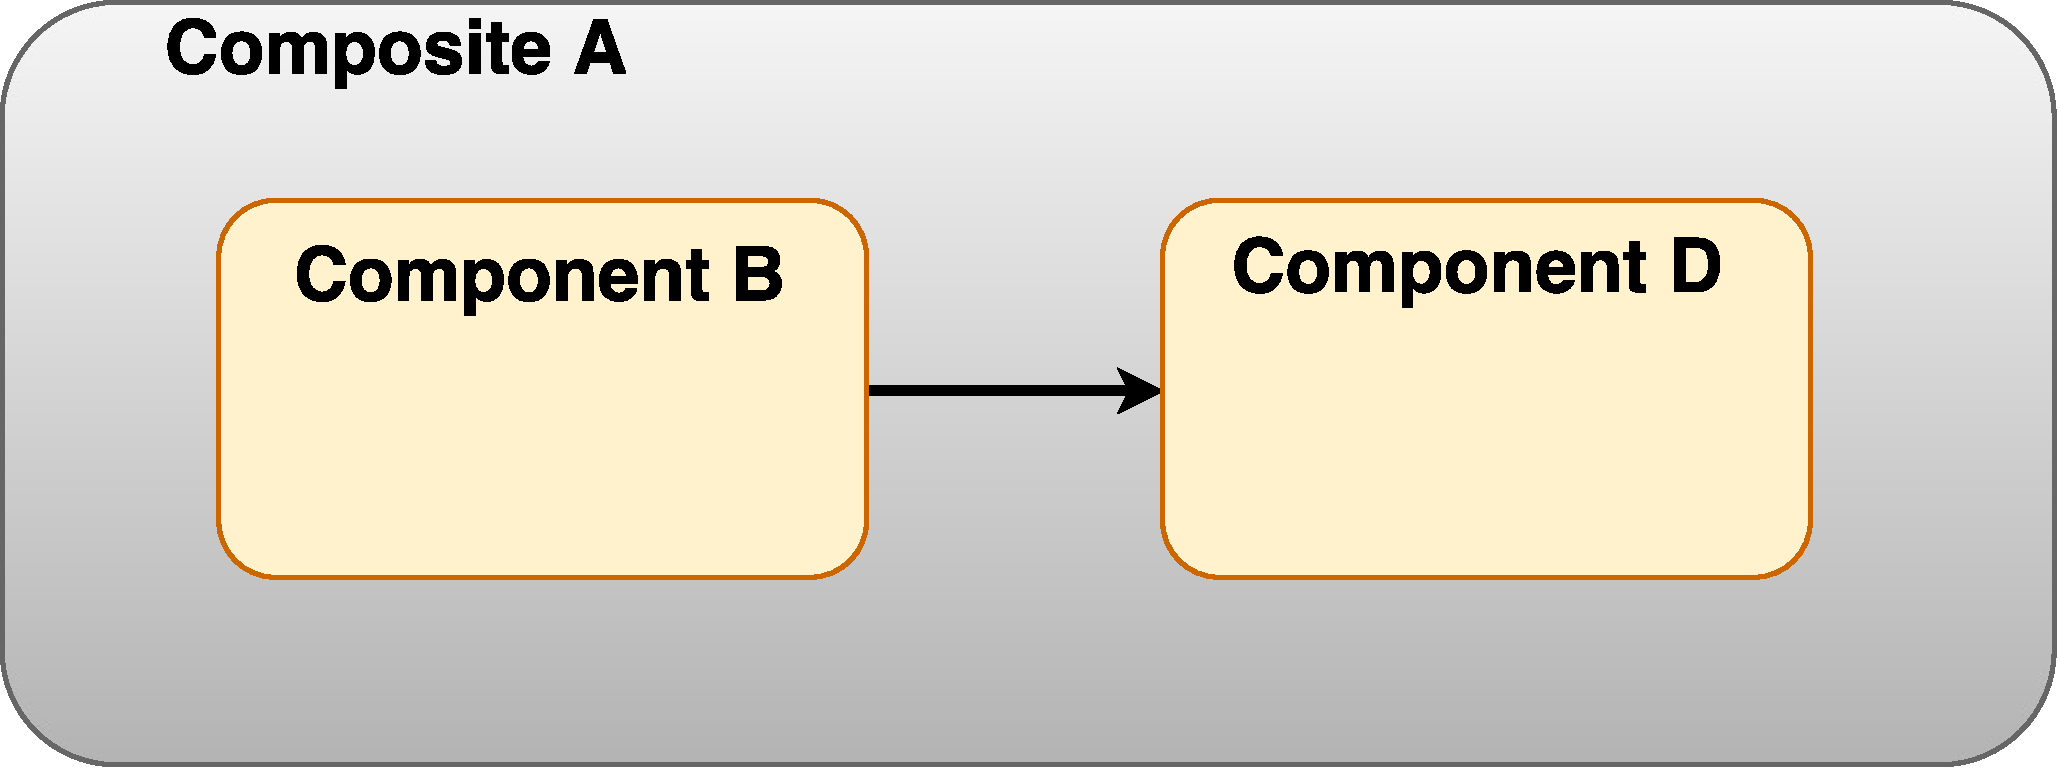
\includegraphics[scale=0.25]{images/CompositeModel}
\caption{Simple Composite.}
\label{fig:CompositeModel} 
\end{figure}
 
A complete application can be constructed from just one composite (figure \ref{fig:CompositeModel}) or through a combination of several different composites (figure \ref{fig:CompositeModel2}). Those are then considerate components if they are integrated in another composite and so on. 
 
\begin{figure}[H]
\centering
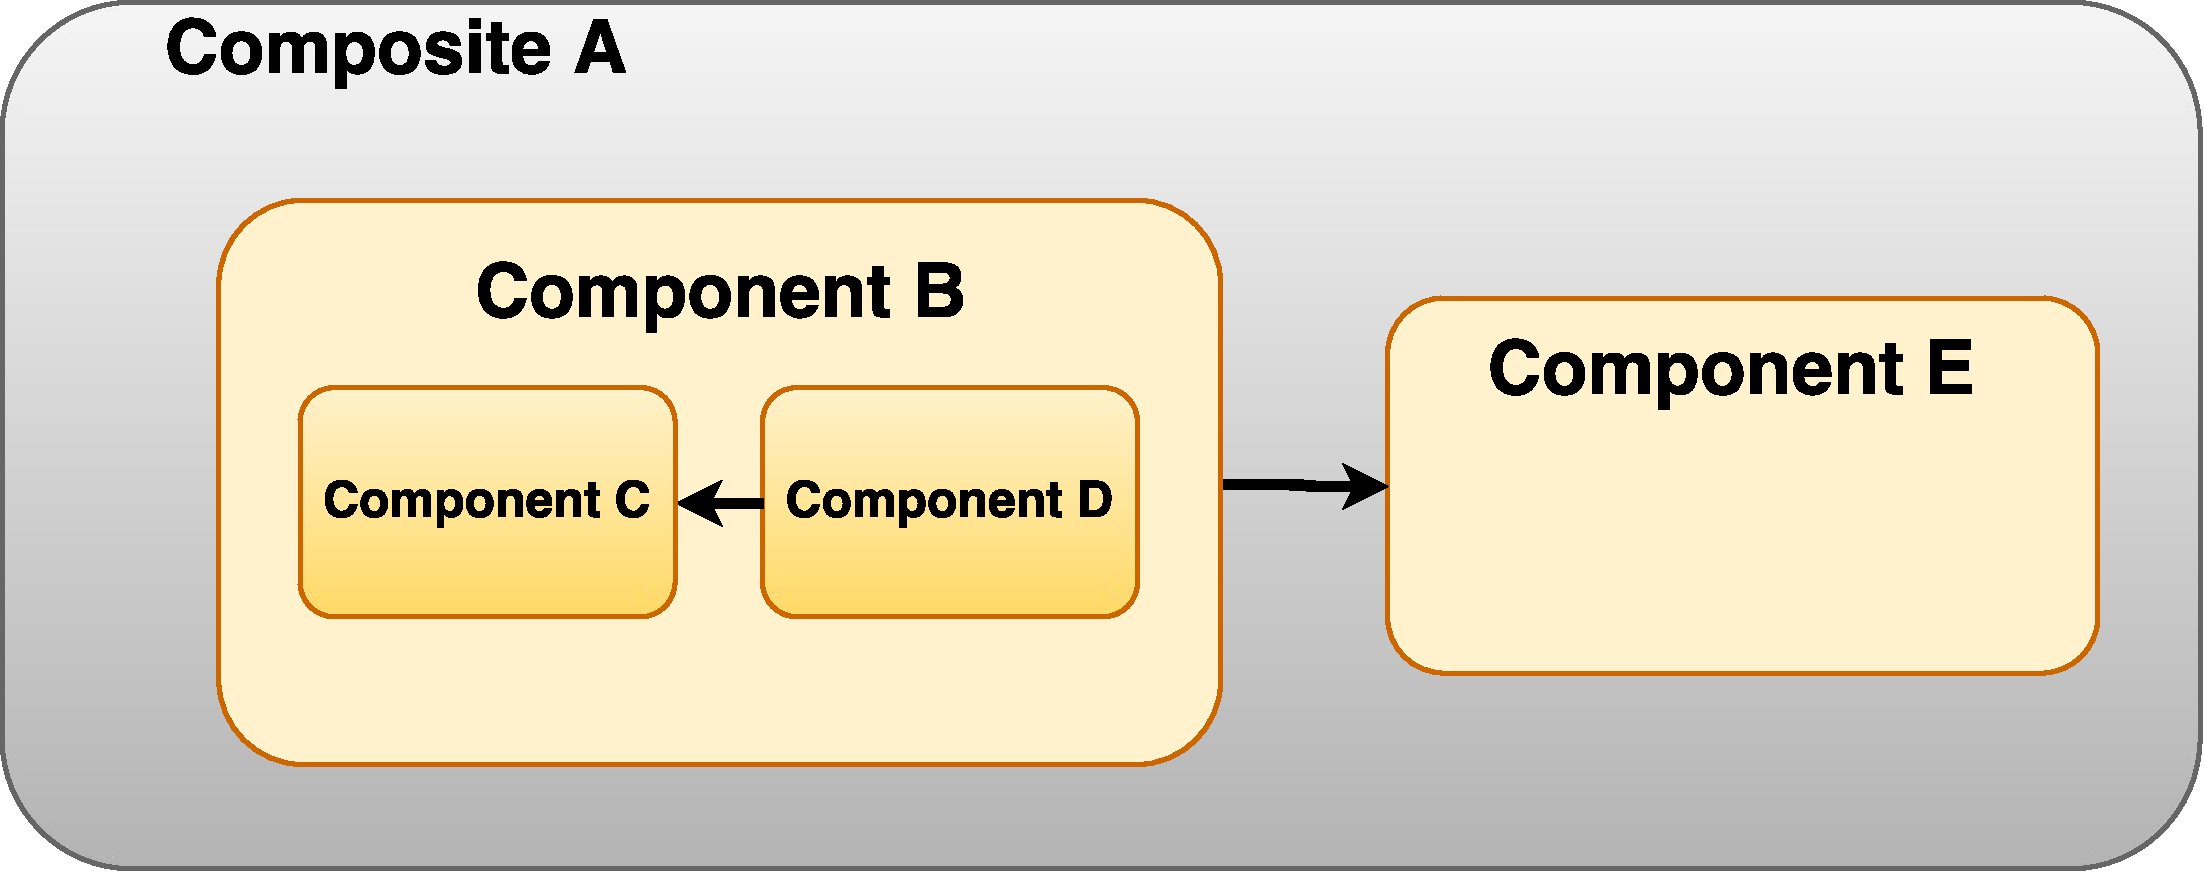
\includegraphics[scale=0.22]{images/CompositeModel2}
\caption{Larger Composite.}
\label{fig:CompositeModel2} 
\end{figure}
 
Components are the atoms from which an \textit{SCA} application is created. Like atoms, \textit{SCA} components behave in consistent ways, and they can be assembled into different configurations. Thus, every component relies on a common set of abstractions, including: \textbf{properties}, \textbf{promotes}, \textbf{services}, \textbf{references} and \textbf{bindings}. \cite{SCA_site} These terms will be recalled later with definitions and respective contextualization with the \textit{EL} Framework. 
 
To sum up, the \textit{SCA} was a reference point for the design of the \textit{EL} framework and for the development of the \textit{EL} language. So, all the conceptual modelization of the particular domains must follow, partly, the \textit{SCA} specifications in order to ensure compatibility with the language, and so, with the framework. In the next sections, it will be covered the full specifications for the definition of the models along with the exhibition of relevant topics related to the \textit{EL} language. Also, the workflow of the EL framework will be illustrated and analyzed aiming the clarification of the process, since the conceptual modelization until the generation of the final source files of a software system.  

\subsection{\textit{EL} Language}

To materialize the conceptual model of a particular domain, an \textit{.el} file must be created. Basically, that process consists in coding the model using the \textit{EL} language. In this section, it will be presented an overview of the language's syntax and semantics as well as its keywords. For consolidation of ideas, along with the explanations, examples of a conceptual model and respective \textit{.el} file will be shown.

\subsubsection{Semantics Overview}

As mentioned, the \textit{SCA} was used as reference point for the development of the language. Its specifications for \textbf{component, properties, references, services, promotes} and \textbf{bindings} were maintained. However, an extension were made to include \textbf{assignments}, as will be presented next. A simple conceptual model (figure \ref{fig:ModelExample}) was created to show how these attributes shall be used.

\begin{figure}[H]
\centering
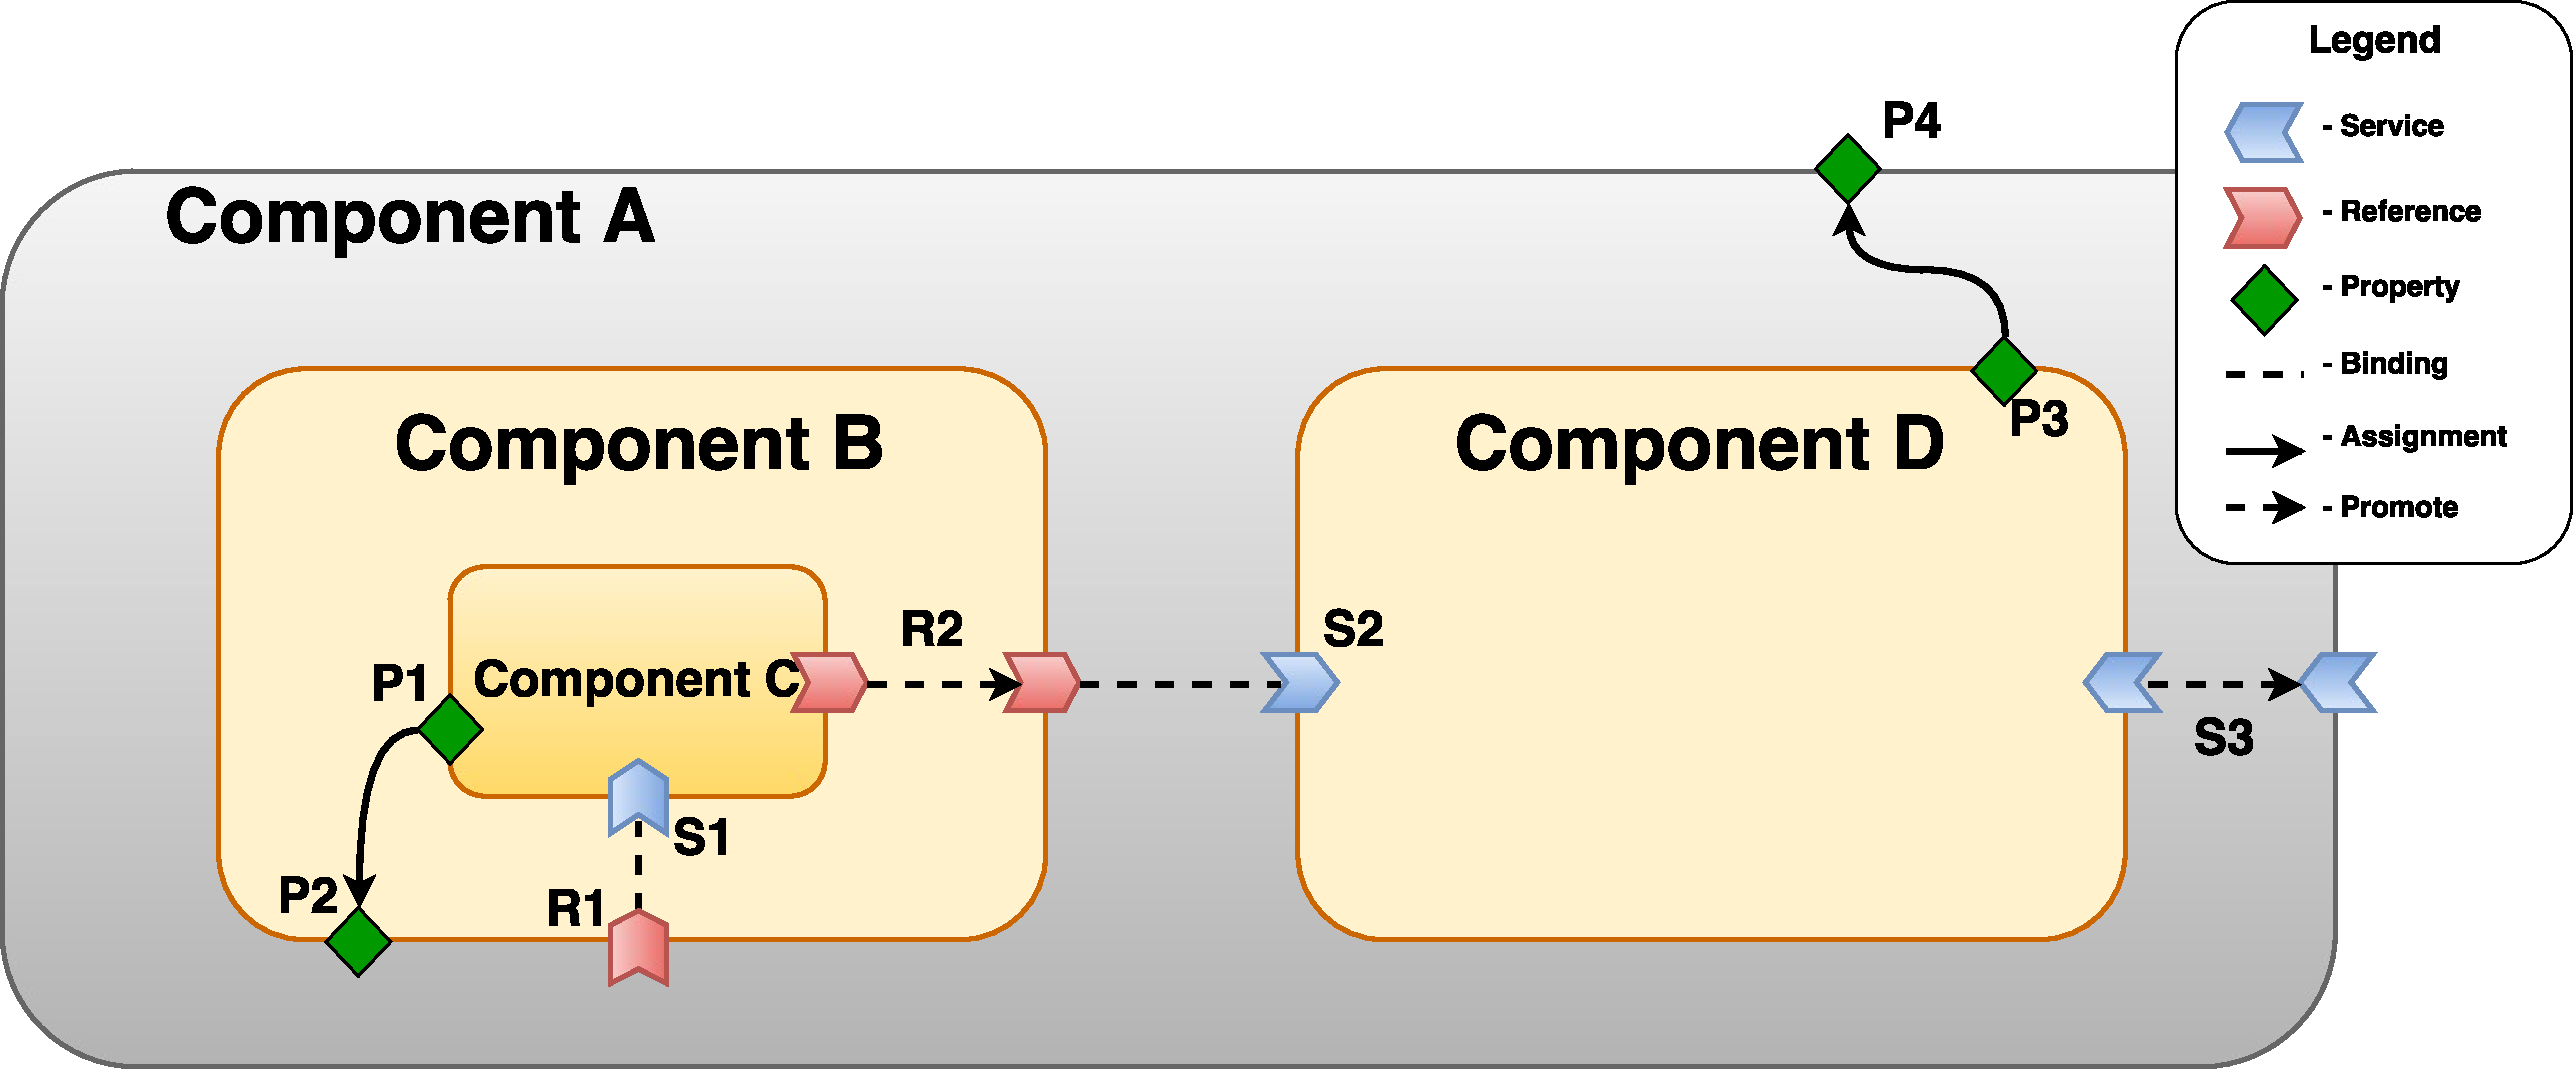
\includegraphics[scale=0.25]{images/ModelExample}
\caption{Simple Conceptual Model.}
\label{fig:ModelExample} 
\end{figure}

\subsubsubsection*{Component}
A top level \textbf{component} can wrap another components, which then can be considered as \textbf{subcomponents}. This way, the top level can access all the properties, references and services of its subcomponents. That is illustrated in figure \ref{fig:ModelExample} where \textit{C} is a subcomponent of \textit{B}, and \textit{B} and \textit{D} are subcomponents of \textit{A}.

\subsubsubsection*{Property and Assignments}
A component's \textbf{property} is an attribute whose value is configurable by the user. During the explanation of the framework's workflow it will become clear the role of the properties. The \textbf{assignments} allows the creation of \textbf{dependencies} between properties. In the simple model, it is visible the dependency between property \textit{P1} and property \textit{P2} and the relation between property \textit{P3} and \textit{P4}.

\subsubsubsection*{References, Services and Bindings}
As referred, one of the main characteristics of the pattern used for the modelization of systems is the existence of interaction between components described as components that need services from other components. This translates in \textbf{references} to \textbf{services}. Figure \ref{fig:ModelExample} shows an example of this type of relation: \textit{B} has a reference \textit{R1} bound to a service \textit{S1} of its subcomponent \textit{C}. This \textbf{binding} is established given the existence of \textbf{interfaces} between them. 

\subsubsubsection*{Promotes}
A \textbf{Promote} allows bindings between references and services that are not accessible through the components scope. This means that when references and services are promoted, their visibility is extended to upper components. In the presented conceptual model, the reference \textit{R2} form \textit{C} is promoted by \textit{B}, therefore, \textit{A} can bind it to the service \textit{S2} provided by \textit{D}.


\subsubsection{Syntax Overview}

In the previous topic, an overview of  \textit{EL} language semantics was made by using a simple conceptual model. Now, this model will be transposed into an ".el" file in order to see the syntax of the language. 

\subsubsubsection*{Language}

The first definition that must be done is the \textbf{language} of the original source files. This entity is necessary for semantics checks since the language of a component must be the same as its subcomponents. It defines the attribute \textbf{annotation} which contains the characters that identifies the location for replacements. 
\begin{lstlisting}[language=EL, caption={Language definition in .el file}, label=lst:lang]
      language C_language
      {	
      				annotation: "##"	
      }    
\end{lstlisting}

\subsubsubsection*{Interface}

Before the definition of the components and its bindings, the \textbf{interfaces} must be created in order to define the services that are provided by the components. Those interfaces can be filled with a list of attributes representing the possible methods/functions implemented in the source files. Listing \ref{lst:inter} shows the interfaces declared for the example in study.

\begin{lstlisting} [language=EL, caption=Interface definition in .el file, label=lst:inter]
      interface interface1{
          function1
      }
      interface interface2{
          function2_1  
          function2_2
      }
      interface interface3{
          function3
      }
\end{lstlisting}


\subsubsubsection*{Component}    

At last, it comes the declaration of the entity component, shown in listing \ref{lst:comp}. The example shows the definition of the component \textit{A}, defined as the top level component of the architecture. 

\begin{lstlisting} [language=EL, caption=Component definition in .el file, label=lst:comp]
      import "language.el"
      import "interface.el"
      import "B.el"
      import "D.el"

      compile A

      component A (C_language)
      {
          subcomponents:
              B b
              D d
          properties:
              string P4
              
          bind b.R2_promoted to d.S2
          promote service d.S3 as S3_promoted
          P4 = d.P3
      }
\end{lstlisting}

The definition of a component goes through several fields that should be filled (not all mandatory):

\begin{itemize}
\item The component's \textbf{name} (\textit{A}) and the source code \textbf{language} (\textit{C\_language}).
\item The \textbf{subcomponents} section used to declare other components that belongs to it (\textit{B} and \textit{D}).
\item The \textbf{properties} section which contains configurable points for the user (\textit{P4}).
\item The \textbf{bindings} section used to wire \textbf{references} (\textit{b.R2}) from one component to \textbf{services} provided by another (\textbf{d.S2}).
\item The \textbf{promote} section where \textbf{references} (\textit{d.S3}) and \textbf{services} declared in its subcomponents can be promoted and visible with a \textbf{new name} (\textit{S3\_promoted}) in upper components.
\item The \textbf{assignment} section where operation on properties are made (\textit{P4 = d.P3}).
\end{itemize}

The example shows also an important keyword in in the language: \textbf{compile}. This keyword is used to inform the compiler which is the top level components that must be used for the generation of the artifacts of the framework, as it will be shown in the following section.

An additional feature is related with imported files. In order to access entities of the model declared in other files (language, interface, component), it is possible to import those files in the top of the \textit{.el} file (\textbf{import} section).


\subsubsection*{Keywords} 

Table \ref{keywordsTable} shows all keywords defined in the \textit{EL} language. Some were already presented in the previous section. This table was obtained from the manual created for the framework in Embedded Systems' course. 

\begin{table}[H]
	\centering
	\caption{EL keywords.}
	\label{keywordsTable}
    \centerline{
	\begin{tabular}{|l|l|}
		\hline
		%\rowcolor[HTML]{C0C0C0} 
		\textbf{Keywords}        & \textbf{Description}		\\ \hline
		\textcolor{red}{annotation} 				 & Defines the character that limits the annotations	\\ \hline
		\textcolor{red}{as}                       & Renames a promoted reference or service \\ \hline
		\textcolor{red}{bind}                     & Binds a reference to a service  \\ \hline
		\textcolor{red}{bool}                     & Component's property data type   \\ \hline
		\textcolor{red}{compile}					 & Tells to compiler which is the top level component \\ \hline
		\textcolor{red}{component}				 & Defines a component	\\ \hline 
		\textcolor{red}{final}					 & Defines that a component has a concrete elaboration \\ \hline
		\textcolor{red}{import} 				     & Imports the content of the specified file	\\ \hline
		\textcolor{red}{int}                      & Component's property data type   \\ \hline
		\textcolor{red}{interface} 			     & Defines a set of functions used by a service or pointed by a reference \\ \hline
		\textcolor{red}{is}						 & Inherits the specified component \\ \hline
		\textcolor{red}{float}                    & Component's property data type   \\ \hline
		\textcolor{red}{language}				 & Defines a language		\\ \hline
		\textcolor{red}{promote}                  & Promotes a reference or service from a subcomponent to a component \\ \hline
		\textcolor{red}{properties}               & Defines the properties set of a component     \\ \hline
		\textcolor{red}{reference}                & Defines the reference used in a promote or in a bind operation  \\ \hline
		\textcolor{red}{references}               & Defines the references set of a component \\ \hline
		\textcolor{red}{restrict}                 & Restricts the values that a property can take to a user's defined set  \\ \hline
		\textcolor{red}{service}                  & Defines the service used in a promote or in a bind operation \\ \hline
		\textcolor{red}{services}                 & Defines the services set of a component  \\ \hline
		\textcolor{red}{string}                   & Component's property data type \\ \hline
		\textcolor{red}{subcomponents}            & Defines the subcomponents set of a component  \\ \hline
		\textcolor{red}{to}                       & Connects a reference to a service in a bind operation \\ \hline
	\end{tabular} }
\end{table} 



\subsection{\textit{EL} Workflow}

In this section it will be presented the magic that is behind the \textit{EL} framework. This way, it is intended to illustrate the flow of events since the \textbf{creation of the \textit{.el} files} until the \textbf{generation of the final sources}, describe some important steps of that process and also enumerate and explain relevant \textbf{artifacts} related to the all mechanism.

\subsubsection{Artifacts}

There is a set of artifacts involved on the functioning of the framework. Those artifacts are: \textbf{\textit{EL} files}, \textbf{Configuration Files}, \textbf{Source Files}, \textbf{Elaboration Files} and the \textbf{Elaborator}. Each one of them has an important role on the workflow and a brief explanation will be presented next.

\subsubsubsection*{\textit{EL} files} 

The \textit{EL} files were already presented in the previous section. As it known, this set of files are an \textit{EL} representation of the model. They will be interpreted by the compiler in order to generate the correct workflow for the elaboration. The workflow will be given by the
components relations and contents.

\subsubsubsection*{Configuration files}

The configuration files are generated by the compiler and it is created one per component. Being in a XML representation, its purpose is to allow the \textbf{configuration of the component's properties} by the user. These properties may represent configurable values in the source files or it can represent a relevant information for the elaboration. Following the example that is being used, listing \ref{lst:conf_file} shows an example of the generated configuration file of the component \textit{C}.

\begin{lstlisting} [language=XML, caption=Configuration file of the component \textit{C}., label=lst:conf_file]
<component type="C">
	<elaboration default="SpecificCElaboratorTemplate">SpecificCElaborator</elaboration>
	<properties>
			<property type="int" name="P1" default="0">
						<value>
								<element>80085</element>
						</value>
			</property>
	</properties>
</component>
\end{lstlisting}

It is also in the configuration files that is chosen the specific elaboration file for the component. Its location in the file is shown in the example, where the user can configure the property \textit{P1}, in the <\textit{value}> field.

\subsubsubsection*{Source files}

These are the artifacts that will be \textbf{manipulated by the elaboration}. A set of source files should be associated with each specific elaboration of each component. These files may represent a possible behavior representation of the component and may \textbf{contain annotations} that will be used by the elaboration to perform the pretended changes. Listing \ref{lst:source_file} shows an example of an annotated source file.

\begin{lstlisting} [language=C,, caption=Annotated source file., label=lst:source_file]
#include <stdio.h>
void print() {
	int number = ##annotation2## ;
  printf("\nnumber choosen = %d\n\n", number);  }
    
void print2() { printf("\nOther Service\n\n"); }

int main() {
	##annotation1##();  return 0;
}
\end{lstlisting}

\subsubsubsection*{Elaboration files}

Each component should have at least one of these files. Written in java, they are responsible for fetching the configurations from the configuration files, and \textbf{perform the respective changes in the source files}. There can be more than an elaboration for each component, but only one should be loaded by the Elaborator. 

To manipulate the annotated sources, it is used an \textbf{Elaboration API} which contains a \textbf{set of methods for elaboration purposes}. Those methods are shown in listing \ref{lst:elabAPI_file}.


\begin{lstlisting} [language=Java, caption=Elaboration API methods, label=lst:elabAPI_file]
public void openAnnotatedSource(String source_path);
public void openAnnotatedSource(String source_path, String targetPath);
public void openAnnotatedSharedSource(String source_path) 
public void replaceAnotation(String annotation, String config);
public void replaceAnotation(String annotation, String config, String targetfile);
public void replaceAnotation(String annotation, int config);
public void replaceAnotation(String annotation, int config, String targetfile);
\end{lstlisting}

Using the Elaboration API, it is possible to get the annotated sources through the \texttt{openAnnotated...()} methods and replace the annotations using the \texttt{replaceAnotation()} functions.

As referred, the configuration files are used to choose the elaborations. When the elaboration process starts (by running the Elaborator), it is called the \texttt{generate()} method present in each specific elaboration class, in a specific order. Listing \ref{lst:elab_file} represents an example of the \texttt{generate()} method inside the \texttt{SpecificCELaborator} class of the component \textit{C}. 

\begin{lstlisting} [language=Java, caption=Elaboration file of the component \textit{C}, label=lst:elab_file]
public void generate()
{
      System.out.println("Running C elaboration !!!");	
      openAnnotatedSource("source_file.c");

      _D D_component = (_D) target.get_R2();
      AbstractDElaborator DElab = (AbstractDElaborator) getElaborator(D_component);	
      replaceAnotation("annotation1",(String)DElab.getInterface2ElaboratorFunction2_1());

      int number = target.get_P1();
      replaceAnotation("annotation2", Integer.toString(number));
}
\end{lstlisting}

Recalling the conceptual model, it is possible to verify that the component \textit{C} has a reference to a service of the component \textit{D} and also has a property \textit{P1}. To prove the point, the first step was to get the source file annotated using the method \texttt{openAnnotatedSource()}. Then, it was fetched the service from the component \textit{D}, by returning the function  that implements that service, and the \texttt{annotation1} was replaced using the method \texttt{replaceAnotation()}. Finally, by getting the value of the property \textit{P1} and replacing it in the \texttt{annotation2} with its value, the elaborator can be called and the generated source file will be generated as follows:

\begin{lstlisting} [language=C, caption=Final source file \textit{C}, label=lst:final_source_file]
#include <stdio.h>
void print()  {
	int number = 80085;
	printf("\nnumber choosen = %d\n\n", number);  }

void print2() {  printf("\nOther Service\n\n");  }

int main() {
	print();  return 0;  
}
\end{lstlisting}

As shown in listing \ref{lst:final_source_file}, the annotations were replaced correctly and the generated source file is ready for compilation and execution. It is important to refer that if it was intended to use \texttt{print2()} function instead of \texttt{print()} function, it was only needed to go to the component C specif elaboration file and get the other function implemented by component \textit{D} (replace \texttt{getInterface2ElaboratorFunction2\_1()} with \texttt{getInterface2ElaboratorFunction2\_2()}). 


\subsubsection*{Elaborator}

At last, another resource generated by the compiler is the \textbf{Elaborator}. This artifact uses all generated (and modified) resources (model classes, XML files and elaboration files) to perform the elaboration process.

The elaborator is represented by a \textbf{java class} and its body contains a specific flow of steps for the generation of the final sources. The first step corresponds to the \textbf{construction of the model} using the java classes generated for each component. Secondly, the \textbf{xml files are parsed} to set the values of the properties. It follows the \textbf{solving of the dependencies} between components, and finally, the \textbf{elaboration classes are loaded} using the java API for reflexion. Having all elaboration files loaded, the last steps consists in calling the method \texttt{generate()} of the top level component which call recursively the method \texttt{generate} of its subcomponents.

That being said, after the configuration of the XML files by the user, the elaborator must be compiled and executed in order to generate the final source files.


\subsubsection{Workflow}

All the referred artifacts should interact according to the designed workflow of the \textit{EL} framework. The representation of the overall system can be seen in figure \ref{fig:workflow}. This figure was obtained from the manual created for the framework in Embedded Systems' course. 

It reflects how the artifacts relate with each other and so its definitions must be well understood. Firstly, a model representation should be converted into \textit{EL} files. These files will \textbf{go through the compiler} which is going to validate them \textbf{syntactically and semantically}. It will be generated the Elaborator, the configuration files , the abstract elaborations and the java classes to each component. The user configures parameters in the configuration files as well as choose the specific elaboration files. Those files are the input to the \textbf{Elaborator}, which is going to \textbf{perform the final generation}.

\begin{figure}[H]
\centerline{
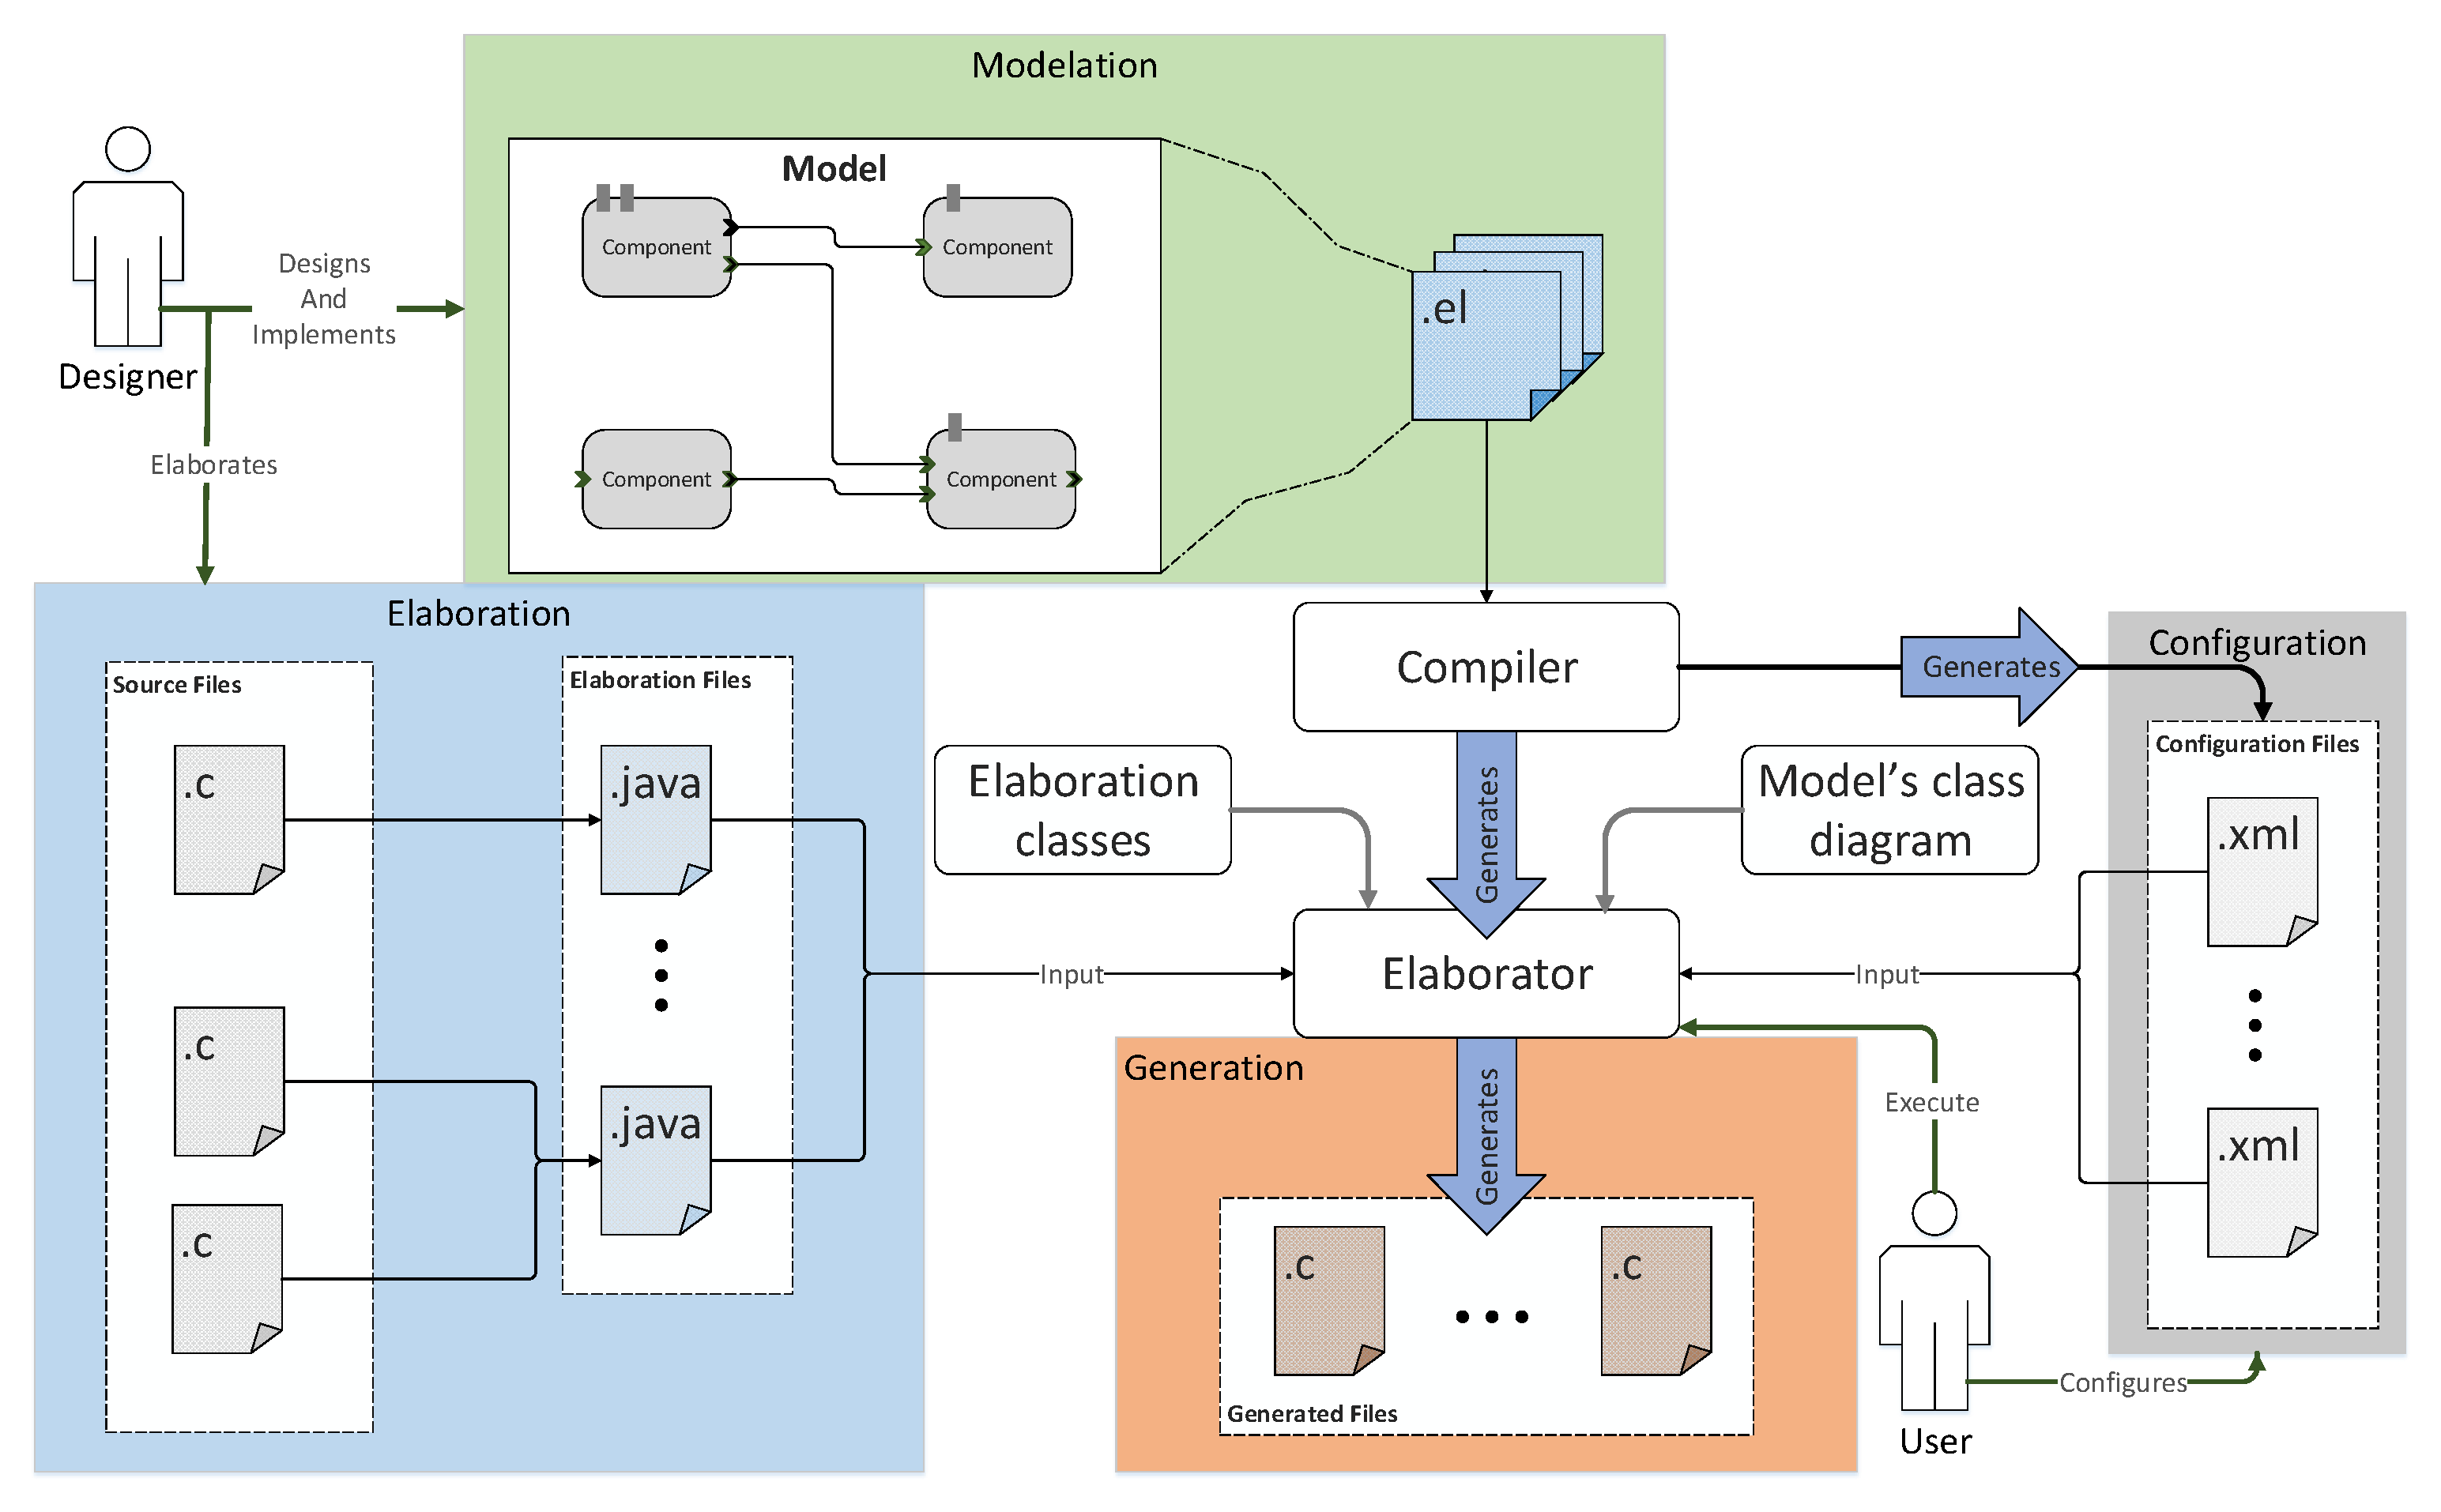
\includegraphics[scale=0.3]{images/EL_workflow} }
\caption{EL framework workflow.}
\label{fig:workflow} 
\end{figure}



\subsubsection{Final File System}

As it was explained in the \textit{Workflow} section, after the compilation of the \textit{.el} files, a several number of other files are generated. For organizational purposes,  folders are also generated and the files are stored inside of each folder respectively. Figure \ref{fig:file_system} illustrates the generated files system of the simple example that as been followed.   


Only some of the sub-folders of the file system are shown in the figure, the more relevant ones. It is possible to see the folders chain of the \textit{Configs} folder. It contains all the configuration files of each component of the model. Is in the \textit{Final Files} folder that will be stored the final source files, after the Elaborator operation. As for the \textit{SpecificElaborations} it is created a folder to each component and, inside of it, must be created folders to store the specific elaboration files along with the annotated sources. If an annotated source file will be manipulated by different elaborations files, that source must be stored in the \textit{SharedSources} folder.

\begin{figure}[H]
\centering
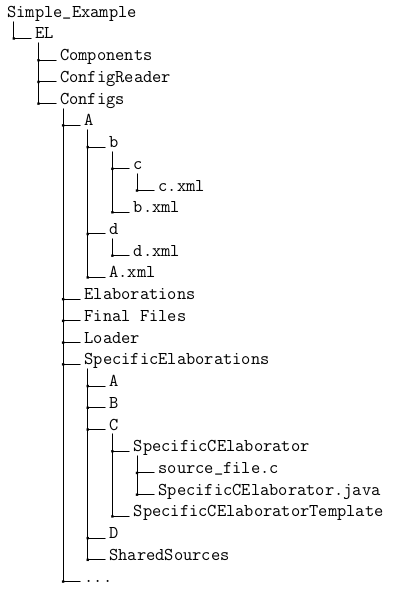
\includegraphics[scale=0.6]{images/files_system}
\caption{Final Files System.}
\label{fig:file_system} 
\end{figure}



\newpage
\section{Dynamic Binary Translator}

As mentioned, the main goal of this project is the modelization of a dynamic binary translator using the language \textit{EL}. In order to accomplish that purpose, the project relies on an already implemented \textit{DBT} to design a reference architecture, developed and provided by the advisor Filipe Salgado. The \textit{DBT} in study has as it source architecture the 8051 \textit{ISA} and has it target the Thumb2 \textit{ISA }(ARM-Cortex M3). 

Architecturally, the \textit{DBT}  can be represented mainly by five blocks and their interaction: \textbf{CCache}, \textbf{TCache}, \textbf{\textit{DBT} Engine}, \textbf{Native Execution} and \textbf{Data Memory} (Figure \ref{fig:DBT_Engine}).

\begin{figure}[!htb]
\centering
\includegraphics[scale=0.7]{images/DBT_engine.png}
\caption{DBT engine model.}
\label{fig:DBT_Engine} 
\end{figure}

Two main blocks that compose the \textit{DBT} are two caches used for faster data access. The first one is called \textit{\textbf{CCache}} and its job is to store portions of source code (any sources such as a \textit{ROM}, serial port or a flash memory). The second one is called \textit{\textbf{TCache}}, a memory responsible for storing translated code (native code for the target architecture).

The execution flow engine can be described as followed: on top of the target processor is running the \textbf{DBT engine}, which accesses the \textit{CCache}, translates the code in units of \textbf{B}asic \textbf{B}locks and stores it in \textit{TCache}. The translated code is ready for execution. That being said, \textbf{the activity of the processor commutes between source code Basic Block translation and translated code Basic Block execution} meaning that the processor is either translating or fetching and executing instructions from \textit{TCache}. Both processes access a simulated source architecture data memory to load or store data, according to the program. \cite{DBT1}





%%%%%%%%%%%%%%%%%%%%%%%%%%%%%%%%%%%%%%%%%%%%%%%%%%%%%%%%%%%%%%%%%%%%%%%%%%%%%%%%%%
% Analysis 
%%%%%%%%%%%%%%%%%%%%%%%%%%%%%%%%%%%%%%%%%%%%%%%%%%%%%%%%%%%%%%%%%%%%%%%%%%%%%%%%%%
\newpage
\section{Requirements Analysis and Project Definition}
Analysis is the first phase of the project. All system's features and goals are established together with the definition of the requirements, constraints, resources and use cases of the project. Therefore, this section is responsible for the definition of the project and its planning.

%%%%%%%%%%%%%%%%%%%%%%%%%%%%%%%%%%%%%%%%%%%%%%%%%%
% Overview
%%%%%%%%%%%%%%%%%%%%%%%%%%%%%%%%%%%%%%%%%%%%%%%%%%
\subsection{Project's Overview}
The main purpose of the project is to model a Dynamic Binary Translator using the language \textit{EL}. Thereby, a conceptual model must be created and written in ".el" files as a reference architecture for a \textit{DBT}. Figure \ref{fig:SOverview} shows an overview of the project.

\begin{figure}[!htb]
\centering
\includegraphics[scale=0.5]{images/SOverview}
\caption{System's Overview.}
\label{fig:SOverview} 
\end{figure}

As shown, the EL files are used as inputs of the EL framework, an automation tool developed in Embedded Systems course. The designer (in this case the elements of the group) must create elaboration files (java classes that performs modification on annotated source files) that will be also used as inputs of the framework together with the source files. Finally, the user can select different configurations for the DBT and a final project will be generated.
There so, this project will present a model for a dynamic binary translator, configurable by users, and specific elaboration files (and also new software and hardware implementation) for some of its main components.




%%%%%%%%%%%%%%%%%%%%%%%%%%%%%%%%%%%%%%%%%%%%%%%%%%
% Use Cases
%%%%%%%%%%%%%%%%%%%%%%%%%%%%%%%%%%%%%%%%%%%%%%%%%%
\subsection{Use Cases}
In this section it is presented the different interactions between the system and their actors in form of use cases. It is important to refer that there are two main actors: the designer and the user. The designer must own technical skills since it is the one associated with the creation/development of the system. The other entity is the user, and as the name suggests, it is the one that uses the application for generation of final embedded software systems.


\subsubsection{Dynamic Binary Translator}

Figure \ref{fig:DBTUseCases} shows the use cases scenario created for the main system: the DBT.

\begin{figure}[!htb]
\centerline{
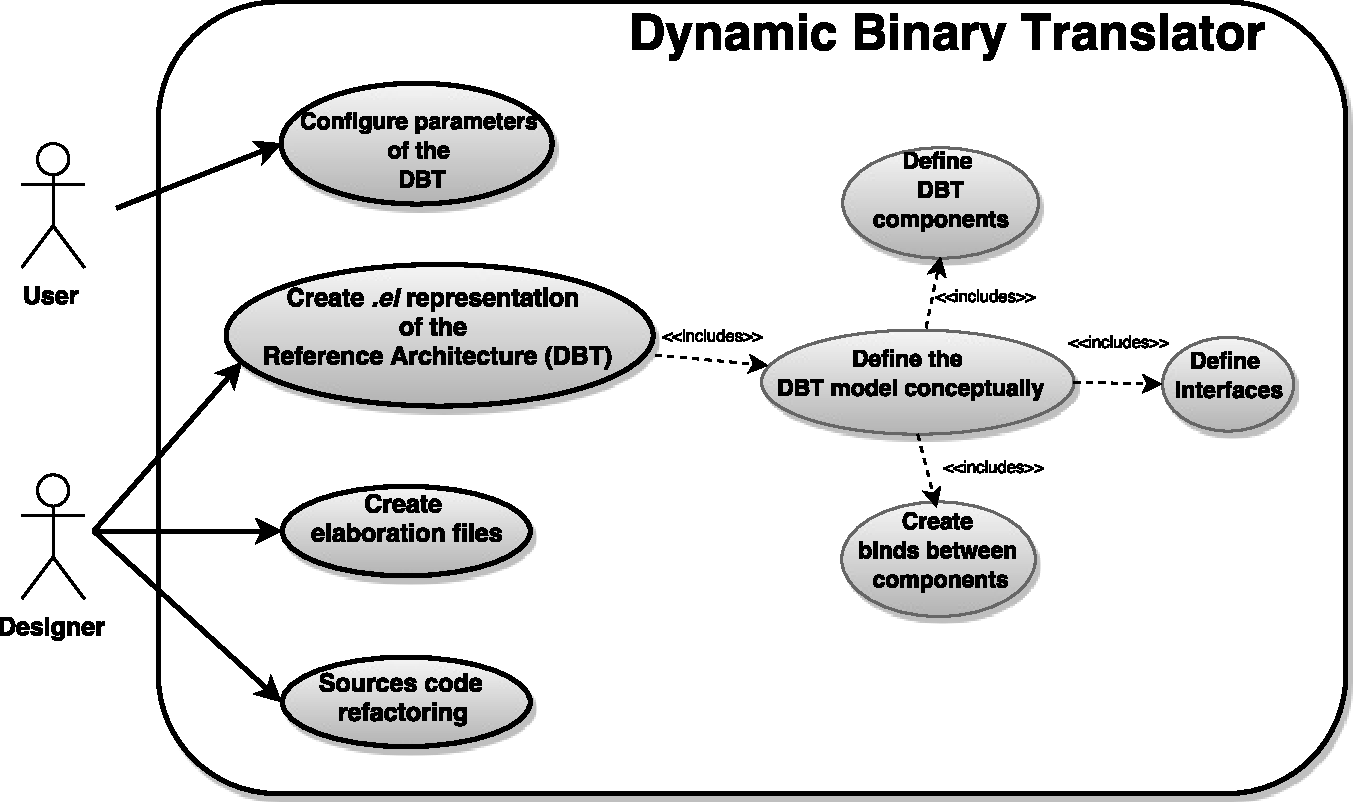
\includegraphics[scale=0.6]{images/DBT_UseCases.pdf} }
\caption{DBT Use Cases.}
\label{fig:DBTUseCases} 
\end{figure}

Since the \textit{EL Framework} is the tool used to model the DBT, a \textit{.el} file containing the reference architecture must be created. But first, to accomplish that task, the model should be well defined conceptually before materialize it in code. So the designer's job must pass through the definition of all the components, as well as the bindings between them. In a certain way, the decision of the bindings leads to the specification of the interfaces. Also, the designer creates the elaboration files for each component and, if required, a refactoring of the source code might be done. This code modification is necessary in situations where there are no compatibility between the model and the code. In the other hand, the user just need to configure some system's parameters, according to his preferences, resulting in a final project with all the code of a customized dynamic binary translator.

%\subsubsection{Decoder}
%
%Since one of the goals of the project is to model the Decoder component, another use case was created to show the role of the designer and user in this subsystem. 
%
%\begin{figure}[!htb]
%\centerline{
%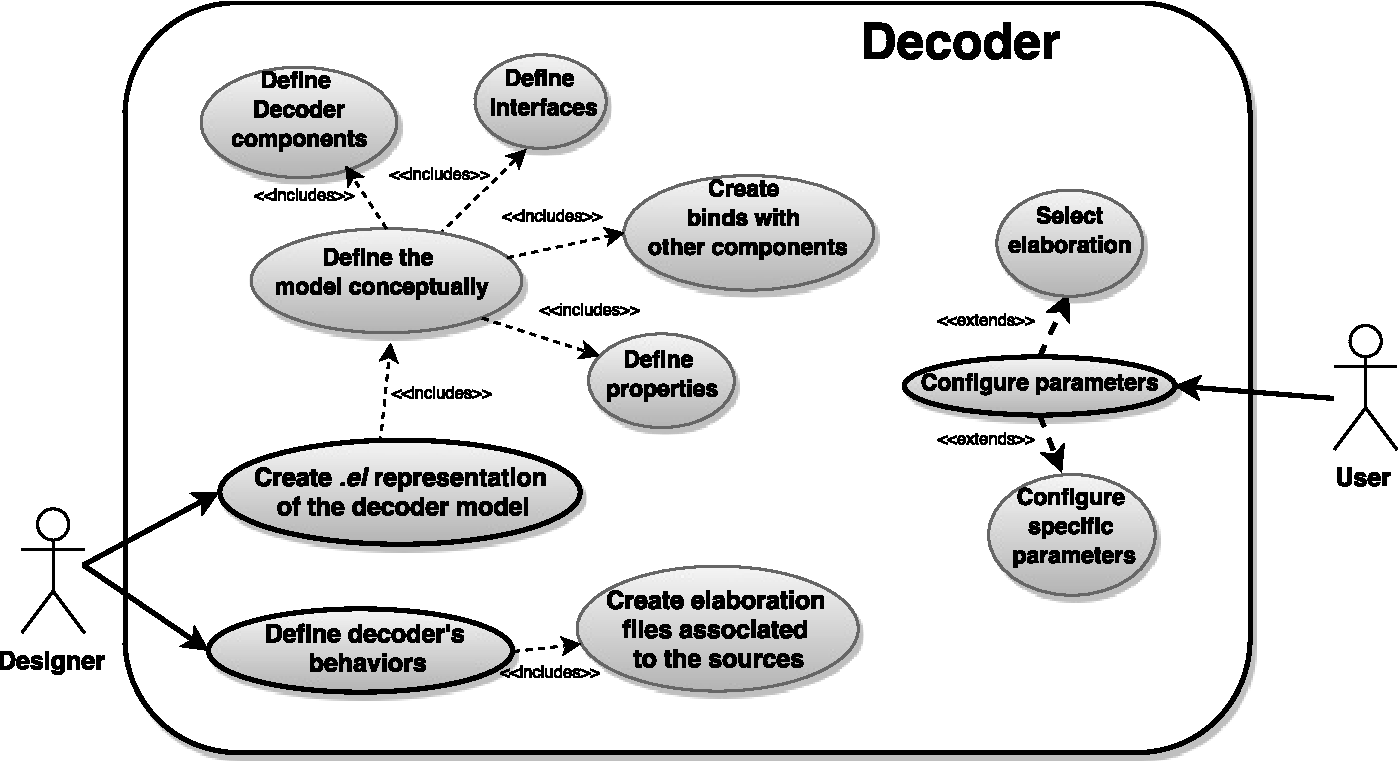
\includegraphics[scale=0.65]{images/Decoder_UseCases.pdf} }
%\caption{Decoder Use Cases.}
%\label{fig:DecoderUseCases} 
%\end{figure}
%
%As figure \ref{fig:DecoderUseCases} shows, the designer has similar tasks as in the DBT: define the Decoder model and create its EL representation. Although, since new implementations can be added, an elaboration file must be created for each one. The role of the user is also the same, the configuration of parameters, however, for new implementations there are some specific properties that must be chosen.


%%%%%%%%%%%%%%%%%%%%%%%%%%%%%%%%%%%%%%%%%%%%%%%%%%
% Requirements
%%%%%%%%%%%%%%%%%%%%%%%%%%%%%%%%%%%%%%%%%%%%%%%%%%
\subsection{Requirements}
The requirement elicitation phase is certainly relevant in the definition of the project since it allows to specify its functional needs. There are two types of requirements defined next: \textbf{Functional Requirements} and \textbf{Non-Functional Requirements}. 

\subsubsection{Functional}
\begin{itemize}
\item Provides a \textbf{model for a Dynamic Binary Translator}, showing its components and functionalities.
\item Provides \textbf{several behaviours for some components of the DBT}, each one represented by its own behavior and interfaces with other components. 
\item Allows the user to \textbf{configure parameters based on his preferences} for the system, which will be transposed to generated code.
\item Provides\textbf{ code generation of final project} (software and hardware implementation) based on the conceptual models created.
\end{itemize}

\subsubsection{Non-Functional}
\begin{itemize}
\item A robust and well defined model of the DBT shall be accomplished.
\item The generated code must be compatible with the target application (DBT), allowing possible hardware migrations of functionalities and automation achieving.
\end{itemize}



%%%%%%%%%%%%%%%%%%%%%%%%%%%%%%%%%%%%%%%%%%%%%%%%%%
% Constraints
%%%%%%%%%%%%%%%%%%%%%%%%%%%%%%%%%%%%%%%%%%%%%%%%%%
\subsection{Constraints}
The project constraints can be classified in two types: \textbf{Technical Constraints} and \textbf{Non-Technical Constrains}. The first ones are related with the technical parts of the project and the second are associated with management issues. Both kinds represent limitations to the developing of the project and so the problems resulting therefrom must be overcome.

\subsubsection{Technical}
\begin{itemize}
\item The DBT must be modeled using the DSL created in embedded system's course and the final project must be generated using the developed framework. 
\item The models can only be implemented after the development of the framework has been finished.
\item The project will be developed around an already implemented Dynamic Binary Translator, that has as its source the 8051 architecture and target the Thumb2 ISA (ARM Cortex-M3).
\end{itemize}

\subsubsection{Non-Technical}
\begin{itemize}
\item The project only has a duration of one semester.
\item The UC has only 5 ECTS (8h/week).
\item The group is composed by two elements.
\end{itemize}

\subsection{Resources}

An overview of the hardware and software resources that will be used in the project  is presented in this chapter. 

\subsubsection{Hardware Resources}

As \textbf{hardware resources}, the following components were identified:
\begin{itemize}
\item Zybo Board (Zynq-7000 ARM), which contains an ARM Cortex-A9 processor (for testing the hardware implementations).

\begin{figure}[!htb]
\centering
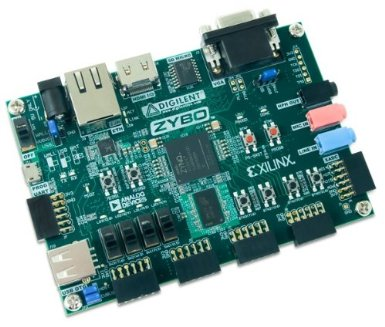
\includegraphics[scale=0.3]{images/Zybo.jpg}
\caption{Zybo Board (Zynq-7000 ARM).}
\label{fig:Zybo} 
\end{figure}

\item Microsemi's SmartFusion\textsuperscript{\textregistered} 2 Advanced Development Kit (ARMV7-M), which contains an ARM Cortex-M3 processor (platform that runs the DBT).
\end{itemize}

\begin{figure}[!htb]
\centering
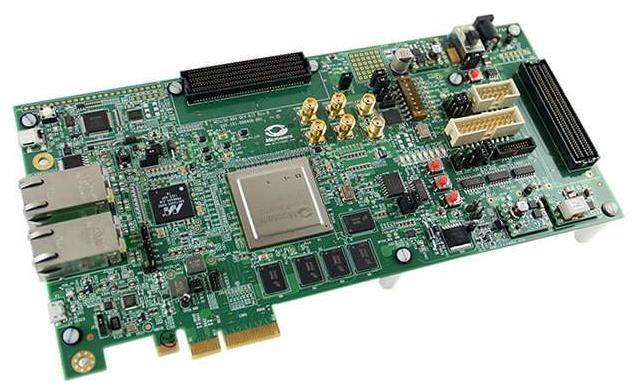
\includegraphics[scale=0.2]{images/SmartFusion2.jpg}
\caption{Microsemi's SmartFusion\textsuperscript{\textregistered} 2 Advanced Development Kit.}
\label{fig:SmartFusion} 
\end{figure}


\subsubsection{Software Resources}
As \textbf{software resources}, several tool will be used to achieve the purposes: 
\begin{itemize}
\item EL Framework.
\item DBT source files.
\end{itemize}


\begin{itemize}
\item Understand™ Static Code Analysis Tool.

\begin{figure}[!htb]
\centering

\includegraphics[scale=0.5]{images/Understand_logo}
\caption{Understand™}
\label{fig:Understand_logo} 
\end{figure}

\item IAR Embedded Workbench (IAR Systems) and C++ Language (for the modification of the DBT project).

\begin{figure}[!htb]
\centering

\includegraphics[scale=0.15]{images/IAR}
\caption{IAR Embedded Workbench }
\label{fig:IAR_logo} 
\end{figure}

\item Vivado Design Suite (Xilinx) and Verilog Language (for the development of the hardware implementation).

\begin{figure}[!htb]
\centering

\includegraphics[scale=0.2]{images/vivado_logo}
\caption{Vivado\textsuperscript{\textregistered} Design Suite}
\label{fig:Vivado_logo} 
\end{figure}

\item Eclipse IDE (for the development of the contents related to the \textit{EL} framework)

\begin{figure}[!htb]
\centering

\includegraphics[scale=0.2]{images/eclipse}
\caption{Eclipse\textsuperscript{\textregistered} IDE}
\label{fig:Eclipse_logo} 
\end{figure}

\end{itemize}


%%%%%%%%%%%%%%%%%%%%%%%%%%%%%%%%%%%%%%%%%%%%%%%%%%
% Planning
%%%%%%%%%%%%%%%%%%%%%%%%%%%%%%%%%%%%%%%%%%%%%%%%%%
\subsection{Planning}
Beyond all the planning of the concerns of the project, it is profitable to outline a initial planning for the accomplishment of the project. It can be beneficial because, in a certain way, forces the definition of some tasks and also allows the correct division of the time given the difficulties of these tasks. That being said, a more methodical and organized approach can be followed.


\begin{figure}[!hb]
\centerline{
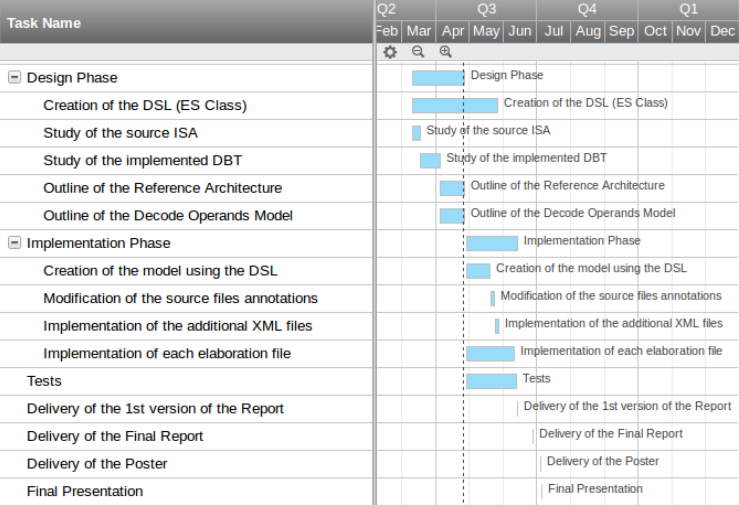
\includegraphics[scale=0.6]{images/planning}}
\caption{Gantt Diagram for the project (post Analysis)}
\label{fig:planning} 
\end{figure}

So, according to our planning, the tasks that can take some of the time are the development of the modelization language, since that it is a project that is being developed from scratch by the entire Embedded Systems class, the study and definition of the conceptual model of the \textit{DBT} and the implementation of the elaboration files as well as the implementations of all the behaviors that the decoder can have, which will be explained rigorously later in this report. 










%%%%%%%%%%%%%%%%%%%%%%%%%%%%%%%%%%%%%%%%%%%%%%%%%%%%%%%%%%%%%%%%%%%%%%%%%%%%%%%%%
% DESGIN
%%%%%%%%%%%%%%%%%%%%%%%%%%%%%%%%%%%%%%%%%%%%%%%%%%%%%%%%%%%%%%%%%%%%%%%%%%%%%%%%%%
\newpage
\section{System and Software Design}

\subsection {DBT Code Analysis}
One of the most crucial steps to be taken before the design of the reference architecture was the analysis of the source code of the DBT project. Thus, this section describes in detail all the software modules identified as well as their role in the final model. 

In a prime instance, it was used a static code analysis tool called \textit{Understand\textsuperscript{TM}} to help to fully comprehend the DBT source code. Among several features, \textit{Understand} provides pertinent information regarding the code and it can be used to easily check the contents and interactions between functions, classes, variables and others. After organizing all the source files in folders and creating a project in \textit{Understand}, the result was as follows:        
 
\begin{figure}[!hb]
\centerline{
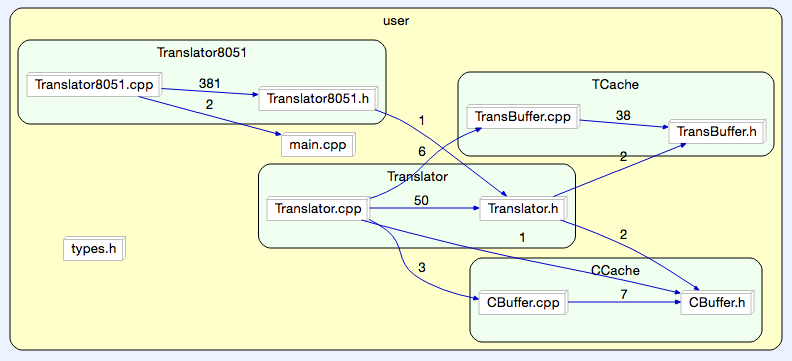
\includegraphics[scale=0.55]{images/understand}}
\caption{DBT Dependency Graph.}
\label{fig:understand} 
\end{figure}

Figure \ref{fig:understand} shows a dependency analysis of the DBT project. Each block highlighted in green contains source and header files, which enclosure a C++ class: \textbf{CBuffer}, \textbf{CTransBuffer}, \textbf{CTranslator} and \textbf{CTranslator8051}. Based on the dependencies observed, it was possible to follow a flow of the code analysis. The major goal at this point was to enhance all the \textbf{components} and find the possible \textbf{interfaces} between them.

\newpage
\subsubsection*{CBuffer}

The \texttt{CBuffer} class (figure \ref{fig:cbufferclass}) is defined and implemented in \texttt{CBuffer.h} and \texttt{CBuffer.cpp}. It is mainly composed by pointers to source code (\texttt{baseBufferAddr} and \texttt{lastBufferAddr}) stored in memory and a method called \texttt{load()} that initializes these pointers with the respective addresses. It also stores the size of the buffer in a variable called \texttt{c\_size}. That being said, this software block can be considered as an \textbf{atomic component}, and the referred method together with the accessors for the memory can be identified has \textbf{services} provided from it.

\begin{figure}[!htb]
\centerline{
\includegraphics[scale=0.53]{images/Cbufferclass}}
\caption{CBuffer Class.}
\label{fig:cbufferclass} 
\end{figure}

\subsubsection*{CTransBuffer}

\texttt{CTransBuffer} class (figure \ref{fig:tbufferclass}) is defined and implemented in \texttt{TransBuffer.h} and \texttt{TransBuffer.cpp}. This class implements an hash table that maps the source code memory address of a Basic Block (key) to translated code memory addresses (value). 

\begin{figure}[!htb]
\centerline{
\includegraphics[scale=0.53]{images/CTransBufferclass}}
\caption{CTransBuffer Class.}
\label{fig:tbufferclass} 
\end{figure}

Like \texttt{CBuffer}, it contains as member variables pointers to the beginning and ending of target code (\texttt{pTargetMem\_begin} and \texttt{pTargetMem\_end}). It also has the address of the source code (\texttt{transSourAddr}) and tree relevant variables: one to store the size of the table (\texttt{t\_size}), another to update the size still available, and at last, the size of the basic block (\texttt{bb\_size}). As member methods, \texttt{TransCache} is composed by several functions used in accessing and managing the hash table (read and write operations) such as \texttt{getCacheAddr(), getCurrInsAddr(), getCodeSize(), addTag(), getTag(), getLastTransAddr(), getTransAddr(), checkForRoom()} and \texttt{cacheCode()}. All of these functions can be seen as services provided by this class to other modules of the code, therefore, \texttt{TrasnCache} is considered also an \textbf{atomic component} and the referred API a \textbf{service}.




\subsubsection*{Translator and Translator8051}

The following figure contains the definition of \texttt{CTranslator} and \texttt{CTranslator8051} classes, two classes that define and implements the engine of the translator together with the specific behavior for the source and target architectures. 

\begin{figure}[!htb]
\centerline{
\includegraphics[scale=0.53]{images/CTranslatorclass}}
\caption{CTranslator, CTranslator8051 and SourceEnvironment classes.}
\label{fig:translatorclass} 
\end{figure}


A new class identified in figure \ref{fig:translatorclass} is \texttt{SourceEnvironment}. This structure contains information about the execution environment of the source architecture, namely, the value of current \textbf{\textit{PC}} (that points to the source code) and another memory structure called \textbf{dataMem}, which represents the data memory of the 8051. Following the same ideas already presented for \texttt{CBuffer} and \texttt{CTransBuffer}, another possible \textbf{component} might be the \texttt{SourceEnvironment}, which provides access to the referred variables by other modules. 

The engine of the translator (translation and execution) is implemented in \texttt{CTranslator}. This class contains an instance of \texttt{CBuffer}, used to access the source code, an instance of \texttt{CTransBuffer}, used to store and read target code, and an instance of a class called \texttt{SourceEnvironment}, that contains information about the execution environment of the source architecture. Also, \texttt{CTranslator} contains another variables used in the engine and defined also for the derived class: \texttt{currBBExecPtr} (pointer to current translated BB), \texttt{eoExec} (flag that signalizes the end of execution) and \texttt{eoBB} (flag that signalizes the end of translation). As member methods the class contains several functions, all with specific functionalities: functions to start and run the DBT (\texttt{initTranslator()}, \texttt{sourceCodeLoader()} and \texttt{runDBT()}), a method responsible for translate BB (\texttt{translate()}), and pure virtual functions that must be overloaded accordingly with the source and target architecture: \texttt{decode()} and \texttt{gen\_prolog()} and \texttt{gen\_epilog()}. Since \texttt{CTranslator} is independent of the architectures and given its behavior as the engine of translation, another \textbf{component} identified is \texttt{DBTEngine}, composed by a \texttt{Translator} and \texttt{Executor}. 

Continuing with the analysis, the last class referred is \texttt{CTranslator8051}, a concrete class derived from \texttt{CTranslator} that implements specific behavior for both architecture. By so, the virtual functions defined in the base class are implemented. The \texttt{decode()} method is responsible for identifying and decoding the operands of the source instruction (specific for source architecture). For that, a set of callback functions were created (\texttt{fineDecode\_0x0(), fineDecode\_0x1()}, etc) each one specific for a type of instruction. At the end, these callbacks are responsible for calling functions used to generate the target code (target behavior), such us, \texttt{gen\_ld8(), gen\_st8()}, among others. All of these functions are used to generate intermediate representation (\textit{IR}) and target code, that is stored in \texttt{CTransBuffer}. Some auxiliary functions are used (helper function - \texttt{gen\_helper()}, etc) to those situations were the behavior is not easy to reproduce with straight assembly code.
Finally, the virtual functions \texttt{gen\_epilog()} \texttt{gen\_prolog()} must also be implemented in \texttt{CTranslator8051}. These function are specific for the target architecture since both insert \textit{ISA} specific code in \texttt{CTransCache} (code that ensures the saving of registers and return address - prologue - and code to restore the program state and flow).

That being said, it becomes easy to identified possible \textbf{components}. Since there are separated code associated with each architecture, two clusters (source and target) can be identified: the \texttt{Source Cluster} is mainly composed by a representation of the \texttt{Source Architecture}, a \texttt{Decoder} and a block representing the \texttt{Source Environments}, and the \texttt{Target Cluster} is composed also by a representation of the  \texttt{Target Architecture} and a  \texttt{Generator}.  

The next section presents a model for the top level component DBT and its subcomponents as well as the bindings between them. 


\subsection{DBT Component}

During the code analysis, all software \textbf{components} were identified and also the \textbf{interfaces} between each other. In additional, several configuration points were found and transposed to the model through \textbf{properties}. Therefore, the necessary arrangements were made and a template solution for an architecture of a DBT was created. Figure \ref{fig:DBT_component} shows the reference architecture purposed.

\begin{figure}[!htb]
\centerline{
\includegraphics[scale=0.45]{images/DBT_v7}
}
\caption{Dynamic Binary Translator component.}
\label{fig:DBT_component} 
\end{figure}

As it can be seen in the figure above, the model were created using rectangles for components, green diamonds for properties, blue steps for services, red steps for references and dotted line for bindings. \\ 

\textit{DBT} is identified as the top level component. Through its modeling, five main subcomponents were identified, all providing the main functionalities of the system: 

\begin{itemize}
\item \textbf{CCache (Code Cache)}: component identified as a buffer that stores source code and manages its use by other components (read operations). It is composed by one property which can be configurable by the user, \textbf{CCache\_Size ($P_2$)}, used by the top level component to check if the basic blocks can be stored in memory. Table \ref{tab:CCachetable} presents the bindings between this component and other components through its services.

\begin{table}[!htb]
\centering
\caption{Services provided from CCache.}
\label{tab:CCachetable}
\begin{tabular}{|c|c|c|}
\hline
\textit{\textbf{Binding}}     & \textit{\textbf{Services}}   &   \textit{\textbf{Components}}     				\\ \hline
$S_{1}$ to $R_{1\_1}$  & fetch  & CCache - Decoder      \\ \hline
$S_{1}$ to $R_{1\_2}$  & load & CCache - \textit{DBT} Engine     \\ \hline
\end{tabular}
\end{table}

\item \textbf{Translation Cache}: component identified as a hash map that stores translated (target) code (in basic blocks) and manages its use by other components (write and read operations). It has one property,  \textbf{TCache\_Size ($P_3$)}, used for the same purpose as \textbf{TCache\_Size ($P_2$)}. It also provides services to other components, shown in table \ref{tab:TCachetable}.

\begin{table}[!htb]
\centering
\caption{Services provided from TCache.}
\label{tab:TCachetable}
\begin{tabular}{|c|c|c|}
\hline
\textit{\textbf{Binding}}     & \textit{\textbf{Services}}   &   \textit{\textbf{Components}}     				\\ \hline
$S_{2}$ - $R_{2\_1}$   & cacheCode  & TCache - Generator      \\ \hline
$S_{2}$ - $R_{2\_2}$  & getTransAddr, addTag & TCache - \textit{DBT} Engine    \\ \hline
$S_{2}$ - $R_{2\_3}$  & \begin{tabular}[c]{@{}c@{}}getLastTransAddr,\\ getCurrInsAddr\end{tabular}  & TCache - Translator               \\ \hline
\end{tabular}
\end{table}


\item \textbf{Source} \textbf{Cluster}: component that aggregates the software blocks associated with the source architecture. All services provided by its subcomponents are shown in table \ref{tab:SrcClustertable}.

\begin{itemize}
\item \textbf{Source Environment}: component that stores information about the execution environment (e.g. PC register and data memory) of the source architecture.
\begin{itemize}
\item \textbf{Data Memory}: component defined as a block of memory representing the \textit{RAM} and \textit{XRAM} of source architecture. It provides methods to access both memories.
\end{itemize}

\item \textbf{Source Architecture}: component which contains all definitions of the source architecture. It contains three main interfaces: one with services related with the source ISA, one representing the registers, and at last, one containing information about the source memory (e.g. Data Memory, External Memory, Heap and Stack). 

\item \textbf{Decode}: component responsible for fetching and decode the source instructions from memory and calling the generator methods that generate the target code. This component has one boolean property, \textbf{srcCodeTracing ($P_4$)}. When set, the source instructions that are send through serial port during translation.

\begin{table}[!htb]
\centering
\caption{Services provided from components of the Source Cluster (Source Architecture, Source Environment, Data Memory and Decoder).}
\label{tab:SrcClustertable}
\begin{tabular}{|c|c|c|}
\hline
\textit{\textbf{Binding}}  & \textit{\textbf{Services}}    &  \textit{\textbf{Components}}    \\ \hline
$S_{3}$ - $R_{3\_1}$       & readDataMem                   &  DataMemory - Generator          \\ \hline
$S_{3}$ - $R_{3\_2}$       & readDataMem                   &  DataMemory - Executor            \\ \hline
$S_{4}$ - $R_{4\_1}$       & nBitsOpcode                   &  Source Architecture - Decoder   \\ \hline 
$S_{4}$ - $R_{4\_2}$       & getWordSize                   &  Source Architecture - CCache    \\ \hline
$S_{5}$ - $R_{5\_1}$          & xDataMemSize,DataMemSize  &  Source Architecture - DataMemory    \\ \hline
$S_{5}$ - $R_{5\_2}$          & MemSize, HeapSize, StackSize  &  Source Architecture - DBT    \\ \hline
$S_{6}$ - $R_{6\_1}$       & SrcRegisters					   &  Source Architecture - Decoder	    \\ \hline
$S_{6}$ - $R_{6\_2}$       & SrcRegisters                     &  Source Architecture - Generator	 \\ \hline
$S_{7}$ - $R_{7\_1}$       & getPC, setPC                  &  Source Environment - Decoder     \\ \hline
$S_{7}$ - $R_{7\_2}$       & getPC                         &  Source Environment - Generator      \\ \hline
$S_{7}$ - $R_{7\_3}$       & envReset                      &  Source Environment - DBT Engine      \\ \hline
$S_{8}$ - $R_{8}$          & decode                        &  Decoder - Translator               \\ \hline
\end{tabular}
\end{table}

\end{itemize}


\item \textbf{Target} \textbf{Clusters}: also a cluster of related software blocks, but in this case, associated with the target architecture. All services provided by its subcomponents are shown in table \ref{tab:TClustertable}.

\begin{itemize}
\item \textbf{Target Architecture}: same representation as the source architecture (same services although provided to other components).
\item \textbf{Generator}: component which provides services for target code generation. Also, it can perform \textbf{optimizations} (property  \textbf{$P_5$}) and \textbf{target code tracing} (property \textbf{$P_6$}) inside those methods.
\end{itemize}

\begin{table}[!htb]
\centering
\caption{Services provided from components of the Target Cluster (Target Architecture and Generator)}
\label{tab:TClustertable}
\begin{tabular}{|c|c|c|}
\hline
\textit{\textbf{Binding}}  & \textit{\textbf{Services}}    &  \textit{\textbf{Components}}    \\ \hline
$S_{9}$ - $R_{9\_1}$  &  \begin{tabular}[c]{@{}c@{}}gen\_addi, gen\_ld8,\\ gen\_st8, gen\_add, \\ gen\_sub, gen\_div, ...\end{tabular}  & Generator - Decoder  \\ \hline
$S_{9}$ - $R_{9\_2}$  &  gen\_prolog, gen\_epilog   & Generator - Translator  \\ \hline
$S_{14}$ - $R_{14}$   &  TrgRegisters  & Target Architecture - Generator  \\ \hline
$S_{15}$ - $R_{15\_1}$  &  getWordSize, nBitsOpcode & Target Architecture - Generator  \\ \hline
$S_{15}$ - $R_{15\_2}$  &  getWordSize   & Target Architecture - TCache  \\ \hline
$S_{16}$ - $R_{16}$    &  \begin{tabular}[c]{@{}c@{}}MemSize, HeapSize,\\ StackSize\end{tabular}  &  Target Architecture - TCache  \\ \hline
\end{tabular}
\end{table}

\item \textbf{\textit{DBT} Engine}: component which represents the engine of the translator. It models the intermediary layer crated in run-time that implements the translation of source code and execution of the target code. Therefore, it is composed by two subcomponents: Translator and Executor. Table \ref{tab:dbtenginetable} shows the services provided by these components.

\begin{itemize}
\item \textbf{Translator}: block responsible for translating the source code. It performs the translation and manages the its flow that occurs continuously inside basic blocks. 
\item \textbf{Executor}: block responsible for executing in the target platform the target code previously translated or already stored in memory from older translations. 
\end{itemize}
\end{itemize}

\begin{table}[!htb]
\centering
\caption{Services provided from components of the DBT Engine Component and its subcomponents (Translator and Executor).}
\label{tab:dbtenginetable}
\begin{tabular}{|c|c|c|}
\hline
\textit{\textbf{Binding}}  & \textit{\textbf{Services}}    &  \textit{\textbf{Components}}    \\ \hline
$S_{10}$ - $R_{10}$   &  initTranslator, runDBT  & DBT Engine - DBT  \\ \hline
$S_{11}$ - $R_{11}$  & translate   & Translator - DBT Engine \\ \hline
$S_{12}$ - $R_{12}$  & execute   & Executor - DBT Engine \\ \hline
$S_{13}$ - $R_{13}$  & currBBExecPtr & DBT Engine - Executor
\\ \hline
$S_{17}$ - $S_{17\_1}$  & eoBB, eoExec & DBT Engine -  Decoder  \\ \hline
$S_{17}$ - $S_{17\_2}$  & eoExec & DBT Engine - Generator \\ \hline
\end{tabular}
\end{table}

At last, a final property were determined for the DBT, \textbf{Measure ($P_1$)}, used to enable time measurement with less possible overhead (code tracing is not allowed in this mode).


This model is identified as a reference architecture for a \textit{DBT}, and for each component, an elaboration file must be created by a designer. Since one of the major intentions of the group is to model the \textbf{Decoder}, this component will be explained in detail next, namely, all interfaces and behaviors.  




\subsection{Decoder Component}

Over the code analysis and modelization of the \textit{DBT} component, the bindings and interfaces established with the Decoder became evident. By inspection, it is possible to see that this component has an interface with the following components: Source Architecture, Source Environment, CCache, Generator and Translator. Next, each binding will be covered one-by-one, being revealed its importance as well as the methods that composes it.

\subsubsection*{Decoder - Source Architecture}
    The Source Architecture is the component that only provides services. The reason for that is based on the fact that its essence consists in the specification of the contents of an architecture. Figure \ref{fig:DecoderBind1}, there are \textbf{two interfaces} between the Decoder and the Source Architecture components (figure \ref{fig:DecoderBind1}).
    
    \begin{figure}[!htb]
    \centerline{
    \includegraphics[scale=0.45]{images/DecoderBind1}
    }
    \caption{Decoder - Source Architecture bindings.}
    \label{fig:DecoderBind1} 
    \end{figure}
    
    The first binding (\textbf{R4\_1 - S4}) lies in an interface which has a function that returns the number of bits of the opcode (\texttt{nBitsOpcode}). This value is used in the generation of the final sources by the elaboration files. In the second binding (\textbf{R6\_1 - S6}), the interface \texttt{Registers} is recognized as an empty interface, \textit{i.e.}, exists and must be respected but there is no way of define functions on it because each architecture has its own registers. In the source files, the definitions of the registers is found in an header file as macros.


\subsubsection*{Decoder - Source Environment}
    As the name suggests, the Source Environment is associated to important elements of the execution environment such as the \textit{PC} and the data memory. 
    
    \begin{figure}[!htb]
    \centerline{
    \includegraphics[scale=0.45]{images/DecoderBind2}
    }
    \caption{Decoder - Source Environment binding.}
    \label{fig:DecoderBind2} 
    \end{figure}
    
    For the Decoder, the value stored \textit{PC} is necessary in decoding branch instructions. Thereby, one of the services that the Source Environment component must provide is the \textit{PC} access which translates in to an interface whose methods must allow get and set the \textit{PC} value, \texttt{getPC} and \texttt{setPC} (figure \ref{fig:DecoderBind2}). 
     
    \subsubsection*{Decoder - CCache}
    In order to decode the operands of an instruction, it is necessary in a prime instance to fetch it. This step is made inside the decoder since the length of the instruction depends of the source ISA, and so, there are situation where this value is not constant. For those situation, the instructions must be fist detected and after fetched. Figure \ref{fig:DecoderBind3} shows the binding established.
    
    \begin{figure}[!htb]
    \centerline{
    \includegraphics[scale=0.45]{images/DecoderBind3}
    }
    \caption{Decoder - CCcache binding.}
    \label{fig:DecoderBind3} 
    \end{figure}
    
    As has been said before, CCache stores portions of binary source code that needs to be translated. Thus, an interface is established and must contain a function that accesses the memory and returns an instruction (\texttt{fetch}). 
       
    \subsubsection*{Decoder - Generator}
    
    Among other responsibilities, the decoder decides which methods must be called for target code generation. This generation service is provided by the Generator which contains the implementations of the generation functions for the target architecture.
	That being said, an interface between the Decoder and the Generator is visible and consists in the \texttt{gen\_x} functions that were mentioned before. Examples of \texttt{gen\_x} functions are shown in figure \ref{fig:DecoderBind4}.
    
    \begin{figure}[!htb]
    \centerline{
    \includegraphics[scale=0.45]{images/DecoderBind4}
    }
    \caption{Decoder - Generator binding.}
    \label{fig:DecoderBind4} 
    \end{figure}
    
    
\subsubsection*{Decoder - DBT Engine}   
    The last service referenced by the Decoder is provided by the DBT Engine (figure \ref{fig:DecoderBind6}). It is composed internal variables of the engine, such as, \texttt{eoBB} (signals the end of a basic block, and so, the end of translation), \texttt{eoExec} (signals the end of execution) and at last \texttt{pSourceProgMem} (pointer to code memory used in instructions that access this the contents of it).
    
	\begin{figure}[!htb]
    \centerline{
    \includegraphics[scale=0.45]{images/DecodeBind6}
    }
    \caption{Decoder - DBT Engine binding.}
    \label{fig:DecoderBind6} 
    \end{figure}
    

\subsubsection*{Decoder - Translator}

	Until now, all the bindings of the Decoder were references to services of other components. But, concerning the correct operation of the DBT engine, the decoder must step in and provide a decoding service to the translator (figure \ref{fig:DecoderBind5}).
    
	\begin{figure}[!htb]
    \centerline{
    \includegraphics[scale=0.45]{images/DecoderBinding5}
    }
    \caption{Decoder - Translator binding.}
    \label{fig:DecoderBind5} 
    \end{figure}
    
    A connection between the Decoder and the Translator is established, consisting in an interface that contains a \texttt{decode} function. So, when a dynamic binary translator is created using the reference architecture that is being design, an implementation of a decode function must inevitably exist.

%%%%%%%%%%%%%
% Decoder Behaviors
%%%%%%%%%%%%%%
\subsection{Decoder Behaviors}

As mentioned, decoding the operands of the source instructions for target code generation can be performed in several ways, therefore, this sections presents some behaviors associated with different implementations (software and hardware approaches). This is done since the EL language allows to define non-final components. This means that, for each behavior, an elaboration file must be created and the source files associated must be annotated accordingly. At the end, the user can select the desired elaboration for this component among the many implemented and theirs specific properties that are specific for the implementation and not referenced in the model.


\subsubsection{Switch Cases}
    This kind of decoder behavior is presented in the original \textit{DBT}, the one that is served as a base to the designed reference architecture. Figure \ref{fig:Decoders_Behavior1} shows the decoder's behavior workflow.

    \begin{figure}[!htb]
        \centerline{
        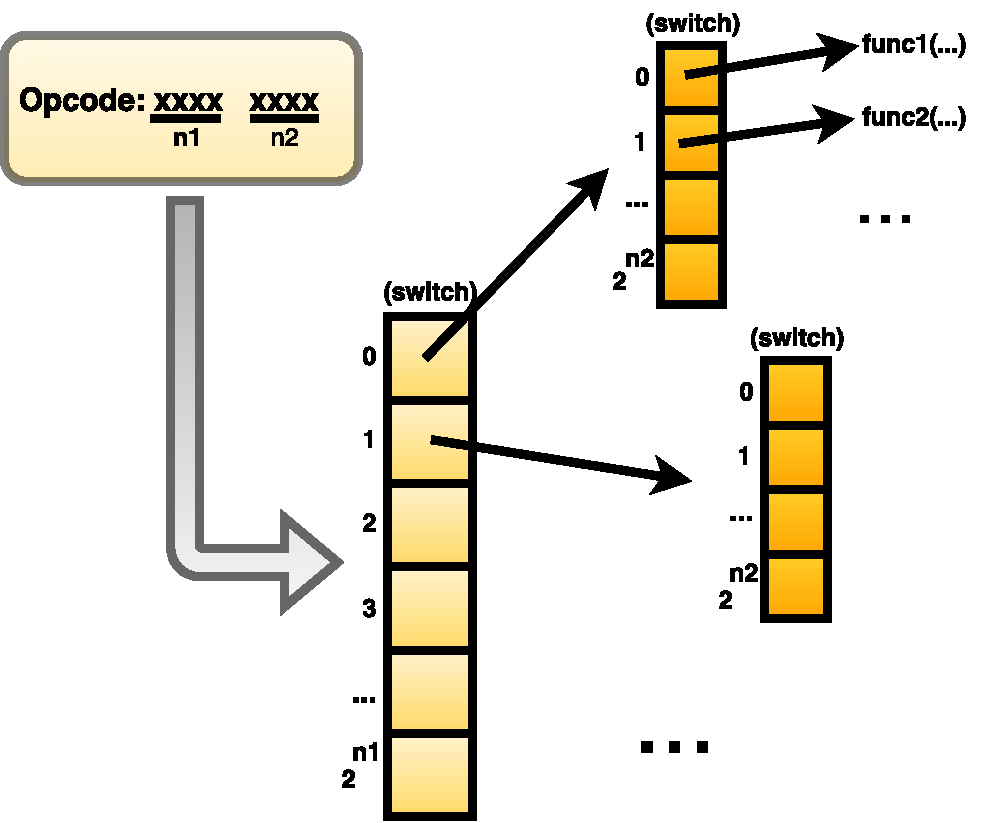
\includegraphics[scale=0.5]{images/Decoders_Behavior1}
        }
        \caption{Decoder's Switch Cases behavior.}
        \label{fig:Decoders_Behavior1} 
        \end{figure}
    
     As the name suggests, the principle operation is based on switch cases which can be only one or several. By so, it follows a simple proposal of a decoder which presents a straightforward operation strategy. It will be seen that it may carry \textbf{some overhead} which can be easily reduced. The opcode is useful because it serves as a guider during the travel along the switch cases. The technique can be described in this 3 steps:
    
    \begin{enumerate}
    
   		\item The opcode is acquired and split. The number of splits will define the number of branches that will occur.
        
        \item It is relevant to know the number of bits of the opcode as well as the number of bits that each portion. Having those values (represented in figure \ref{fig:Decoders_Behavior1} as \textbf{N1} and \textbf{N2}), the size of the first switch case will be 2$^{N1}$. From there, each entry in the switch case will contain another switch case with the size of 2$^{N2}$. If there is no divisions, there will be only one switch case with the length equaling the number of instructions. N1 and N2 are specific properties configurable by the user.

		\item Finally, having the switch cases structure defined, the output is a callback function for a specif instruction. This method implements exactly the steps for decode the instruction. Thereby, given an opcode the result is, in a certain way, a jump to a function.
	\end{enumerate}
    
    To sum up, this process can introduce some overhead if only exists one switch case. This may happens since to reach the correct entry of the switch case, the traversal can be bigger for some instructions. This overhead can be reduced by creating another switch case inside. 

   
\subsubsection{Jump Table}

Between the several behaviors for the Decoder component that will be presented in this chapter, a non implemented one is based on a jump table (figure \ref{fig:Decoders_Behavior2}). A jump table (or branch table) is basically a method of transferring program control to another part of the program (loaded dynamically). There are situations where the compiler creates jump tables from optimized switch statements, however, that can not always be guaranteed. Attending the problem stated in this section, a jump tables was design as a new possible implementation for the decoder. 

Instead of using a switch case to detect the instruction and calling the corresponding generating method, an array is used as the data structure that stores callback functions, indexed with the opcode of the instruction. This behavior can easily be implemented since the callback functions are the same used in the "switch decoder". 

\begin{figure}[
H]
\centerline{
\includegraphics[scale=0.45]{images/Decoder_Behavior2}
}
\caption{Decoder's Jump Cases behavior.}
\label{fig:Decoders_Behavior2} 
\end{figure}


\subsubsection{Generic Decoder}

Another possible implementation for a decoder follows a generic one (Figure \ref{fig:Decoders_Behavior4}), that can be used for any architecture in this reference architecture.  


\begin{figure}[!htb]
\centerline{
\includegraphics[scale=0.45]{images/Decoders_Behavior4_2}
}
\caption{Decoder's Generic behavior.}
\label{fig:Decoders_Behavior4} 
\end{figure}

This type of decoder follows the same principle of a vector indexed by the opcode. However, instead of an address of a function, the vector contains a structures with information about the instruction. 

The structure in each node is composed by two tables named:
\begin{itemize}
\item \textbf{Step Table}, which stores the specific steps that must be performed since the fetch of the instruction until the generation of target code.
\item \textbf{Variable Matrix}, which stores references for variables used inside those steps. Each raw belongs to a function of the step table.
\end{itemize}

In this approach, the hard work relies in building the main table since every instruction must be analyzed and transposed into the structure.  


    \subsubsection{Instruction Format}
    For this last decode procedure, an exhausting study of the source ISA was required. That study was focused on the creation of groups according to the instructions format of 8051 (for this case of study).
    
   
    \begin{figure}[!htb]
    \centerline{
    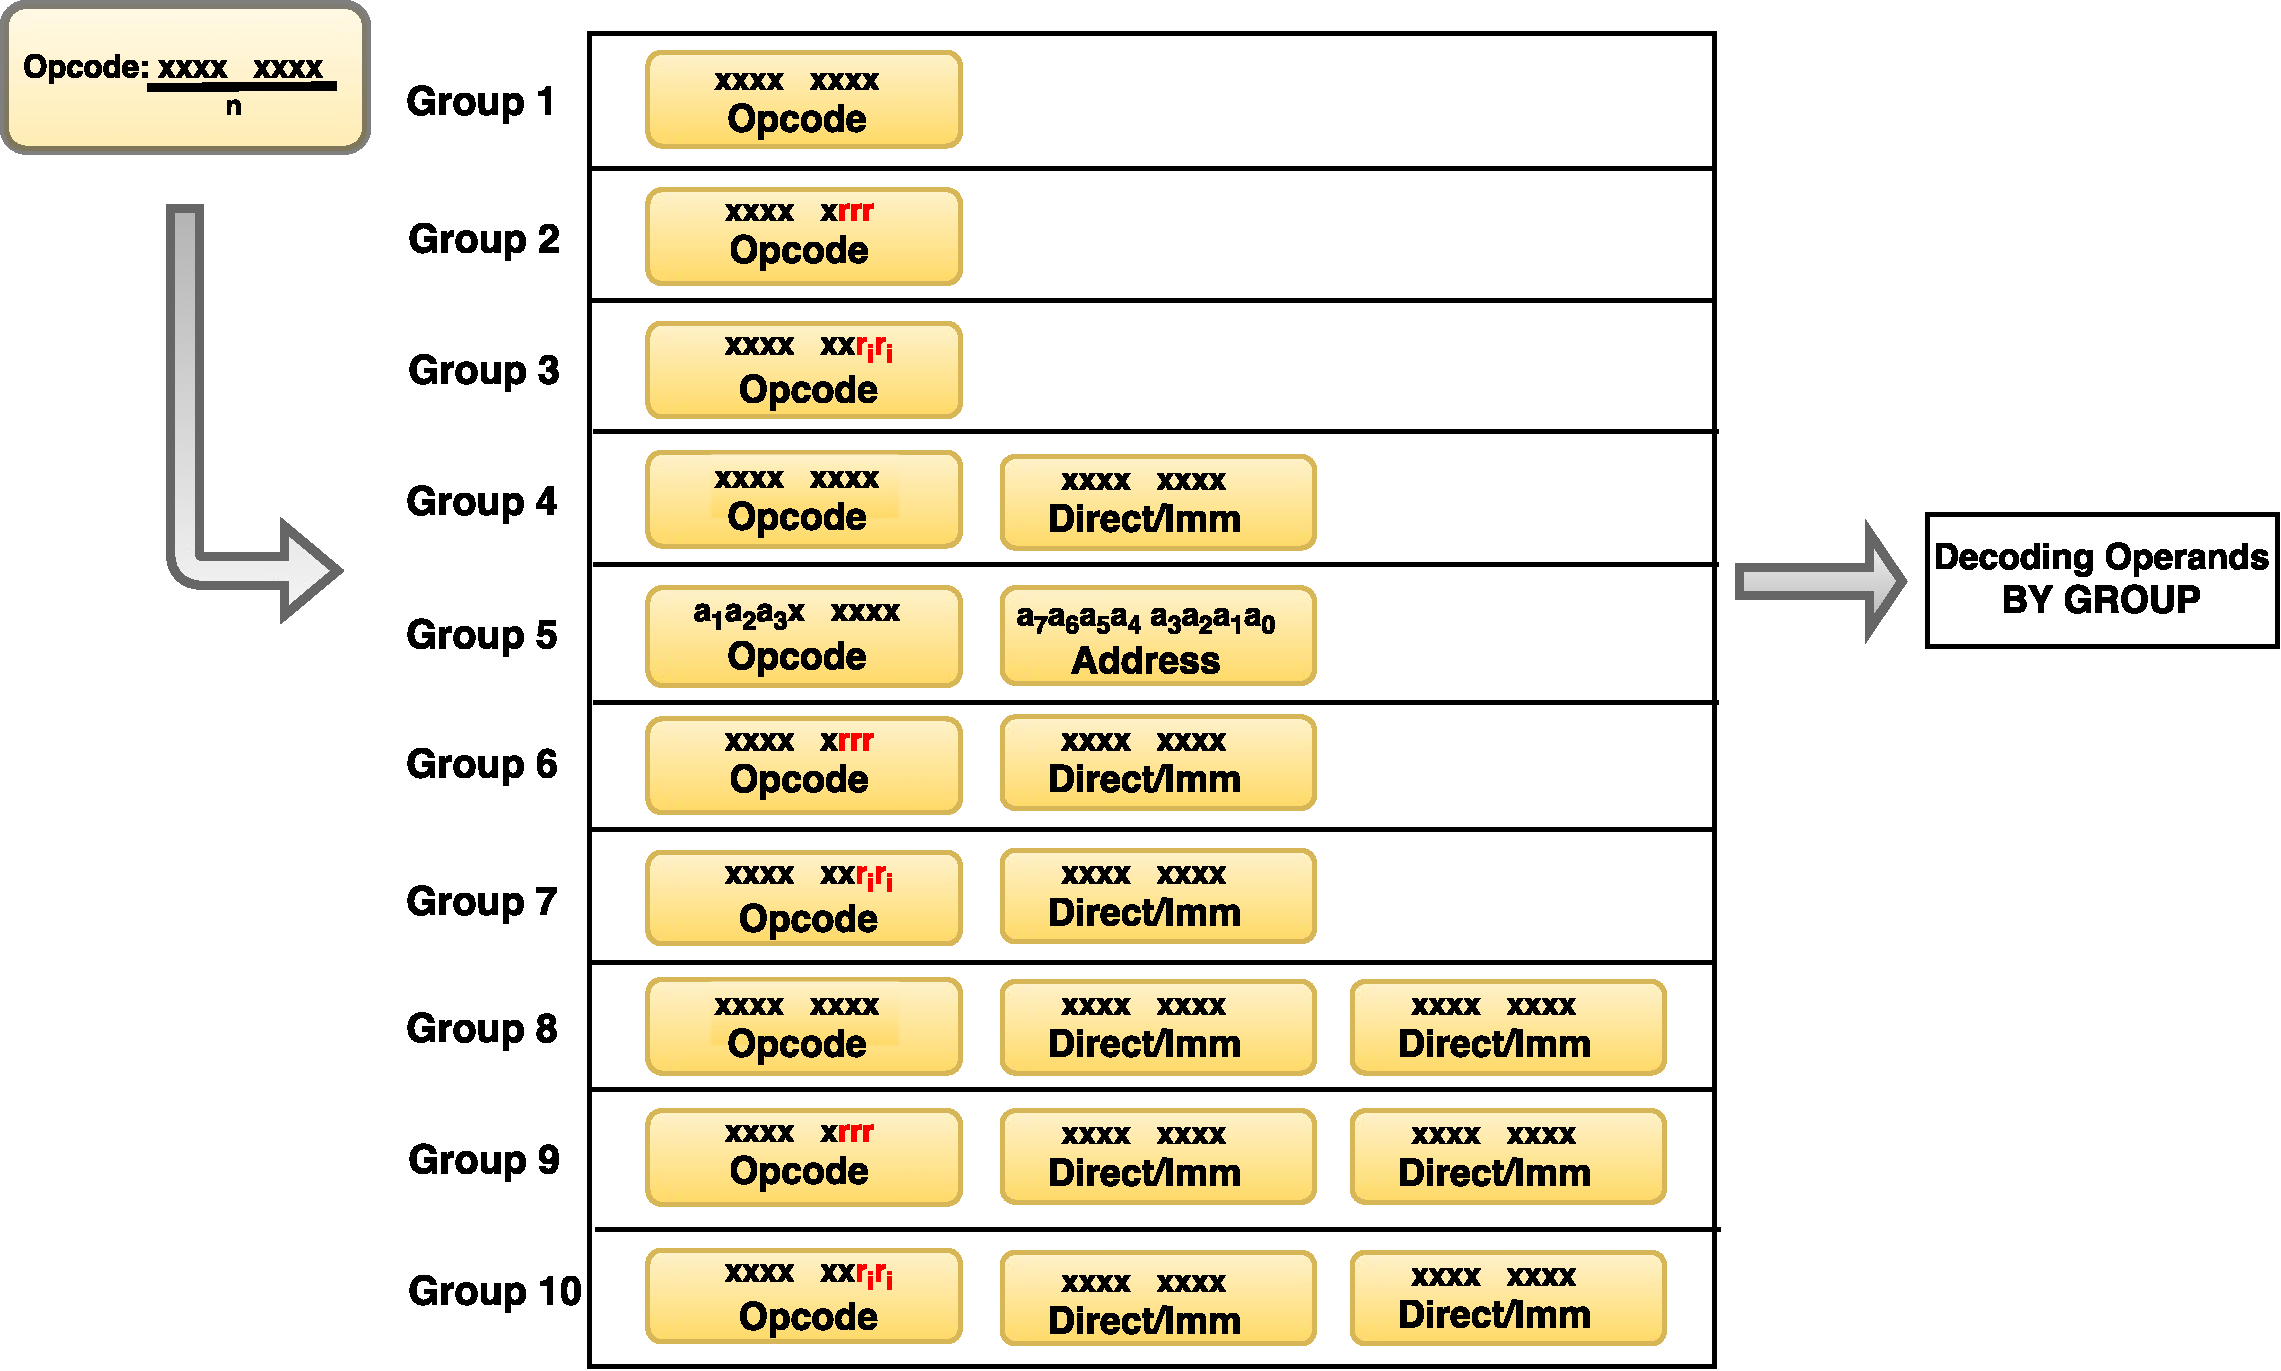
\includegraphics[scale=0.4]{images/Decoders_Behaviors3}
    }
    \caption{Decoder's Instruction Format behavior.}
    \label{fig:Decoders_Behavior3} 
    \end{figure}
	
    This type of decoder is also not implemented. Therefore, in order to achieve that gold, and since its behavior is based on the format of the instructions, there was also the need to check each instruction, evaluate it and according to its format, put it in the specif group. At the end, the result was the existence of 10 groups with the corresponding instruction format, as shown in figure \ref{fig:Decoders_Behavior3}. 
	Having the definition of the groups, the process is quite trivial. Basically, the opcode is acquired, and accordingly with its group, the operands are obtained. Due the selection of the group and other actions that must be executed, this behavior can cost a big price with a software implementation and can become a disadvantage. So, theoretically, a good alternative can be an hardware implementation. However, this implementation requires a different interface in the model (since the target instructions are created without intermediate representation using the operands obtained from the source instruction). For that, an appropriate (and additional) implementation in the generator shall be obtained to accomplish this approach. 

\subsection{Behaviors}
\subsubsection{Decoder Behaviors}
%%%%%%%%%%%%%
% Decoder Behaviors
%%%%%%%%%%%%%%
As mentioned, decoding the operands of the source instructions for target code generation can be performed in several ways, therefore, this sections presents some behaviors associated with different implementations (software and hardware approaches). This is done since the EL language allows to define non-final components. This means that, for each behavior, an elaboration file must be created and the source files associated must be annotated accordingly. At the end, the user can select the desired elaboration for this component among the many implemented and theirs specific properties that are specific for the implementation and not referenced in the model.


\subsubsubsection{Switch Cases}
    This kind of decoder behavior is presented in the original \textit{DBT}, the one that is served as a base to the designed reference architecture. Figure \ref{fig:Decoders_Behavior1} shows the decoder's behavior workflow.

    \begin{figure}[!htb]
        \centerline{
        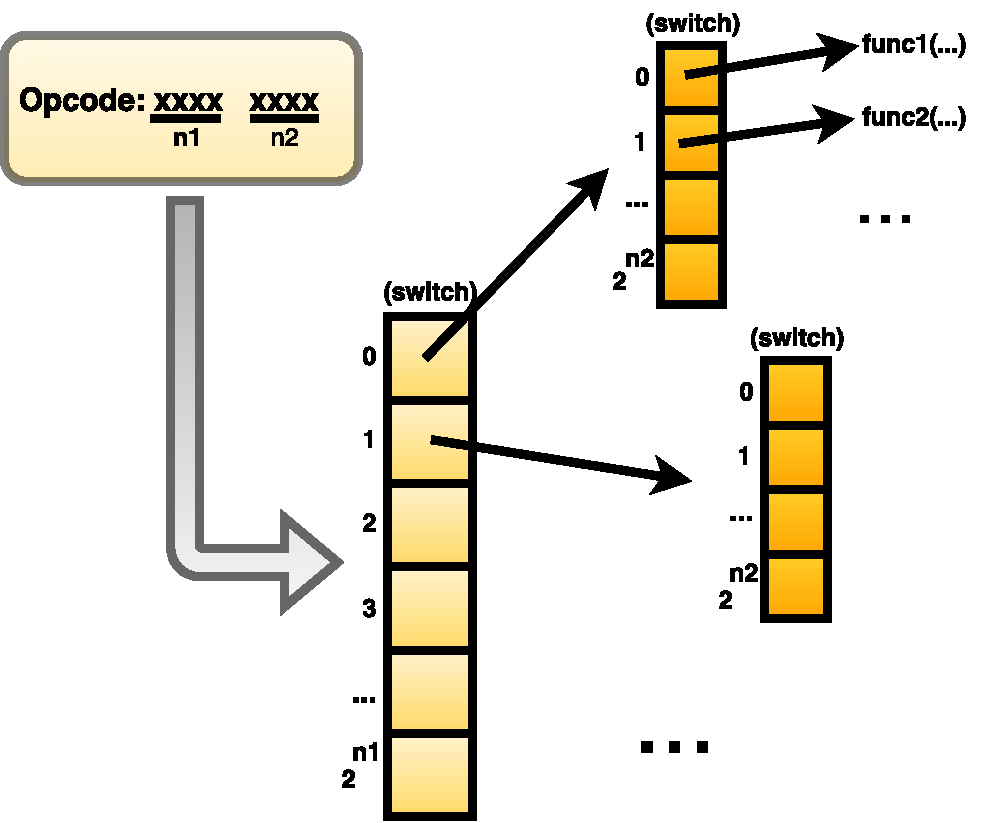
\includegraphics[scale=0.5]{images/Decoders_Behavior1}
        }
        \caption{Decoder's Switch Cases behavior.}
        \label{fig:Decoders_Behavior1} 
        \end{figure}
    
     As the name suggests, the principle operation is based on switch cases which can be only one or several. By so, it follows a simple proposal of a decoder which presents a straightforward operation strategy. It will be seen that it may carry \textbf{some overhead} which can be easily reduced. The opcode is useful because it serves as a guider during the travel along the switch cases. The technique can be described in this 3 steps:
    
    \begin{enumerate}
    
   		\item The opcode is acquired and split. The number of splits will define the number of branches that will occur.
        
        \item It is relevant to know the number of bits of the opcode as well as the number of bits that each portion. Having those values (represented in figure \ref{fig:Decoders_Behavior1} as \textbf{N1} and \textbf{N2}), the size of the first switch case will be 2$^{N1}$. From there, each entry in the switch case will contain another switch case with the size of 2$^{N2}$. If there is no divisions, there will be only one switch case with the length equaling the number of instructions. N1 and N2 are specific properties configurable by the user.

		\item Finally, having the switch cases structure defined, the output is a callback function for a specif instruction. This method implements exactly the steps for decode the instruction. Thereby, given an opcode the result is, in a certain way, a jump to a function.
	\end{enumerate}
    
    To sum up, this process can introduce some overhead if only exists one switch case. This may happens since to reach the correct entry of the switch case, the traversal can be bigger for some instructions. This overhead can be reduced by creating another switch case inside. 

   
\subsubsubsection{Jump Table}

Between the several behaviors for the Decoder component that will be presented in this chapter, a non implemented one is based on a jump table (figure \ref{fig:Decoders_Behavior2}). A jump table (or branch table) is basically a method of transferring program control to another part of the program (loaded dynamically). There are situations where the compiler creates jump tables from optimized switch statements, however, that can not always be guaranteed. Attending the problem stated in this section, a jump tables was design as a new possible implementation for the decoder. 

Instead of using a switch case to detect the instruction and calling the corresponding generating method, an array is used as the data structure that stores callback functions, indexed with the opcode of the instruction. This behavior can easily be implemented since the callback functions are the same used in the "switch decoder". 

\begin{figure}[
H]
\centerline{
\includegraphics[scale=0.45]{images/Decoder_Behavior2}
}
\caption{Decoder's Jump Cases behavior.}
\label{fig:Decoders_Behavior2} 
\end{figure}


\subsubsubsection{Generic Decoder}

Another possible implementation for a decoder follows a generic one (Figure \ref{fig:Decoders_Behavior4}), that can be used for any architecture in this reference architecture.  


\begin{figure}[!htb]
\centerline{
\includegraphics[scale=0.45]{images/Decoders_Behavior4_2}
}
\caption{Decoder's Generic behavior.}
\label{fig:Decoders_Behavior4} 
\end{figure}

This type of decoder follows the same principle of a vector indexed by the opcode. However, instead of an address of a function, the vector contains a structures with information about the instruction. 

The structure in each node is composed by two tables named:
\begin{itemize}
\item \textbf{Step Table}, which stores the specific steps that must be performed since the fetch of the instruction until the generation of target code.
\item \textbf{Variable Matrix}, which stores references for variables used inside those steps. Each raw belongs to a function of the step table.
\end{itemize}

In this approach, the hard work relies in building the main table since every instruction must be analyzed and transposed into the structure.  


    \subsubsubsection{Instruction Format}
    For this last decode procedure, an exhausting study of the source ISA was required. That study was focused on the creation of groups according to the instructions format of 8051 (for this case of study).
    
   
    \begin{figure}[!htb]
    \centerline{
    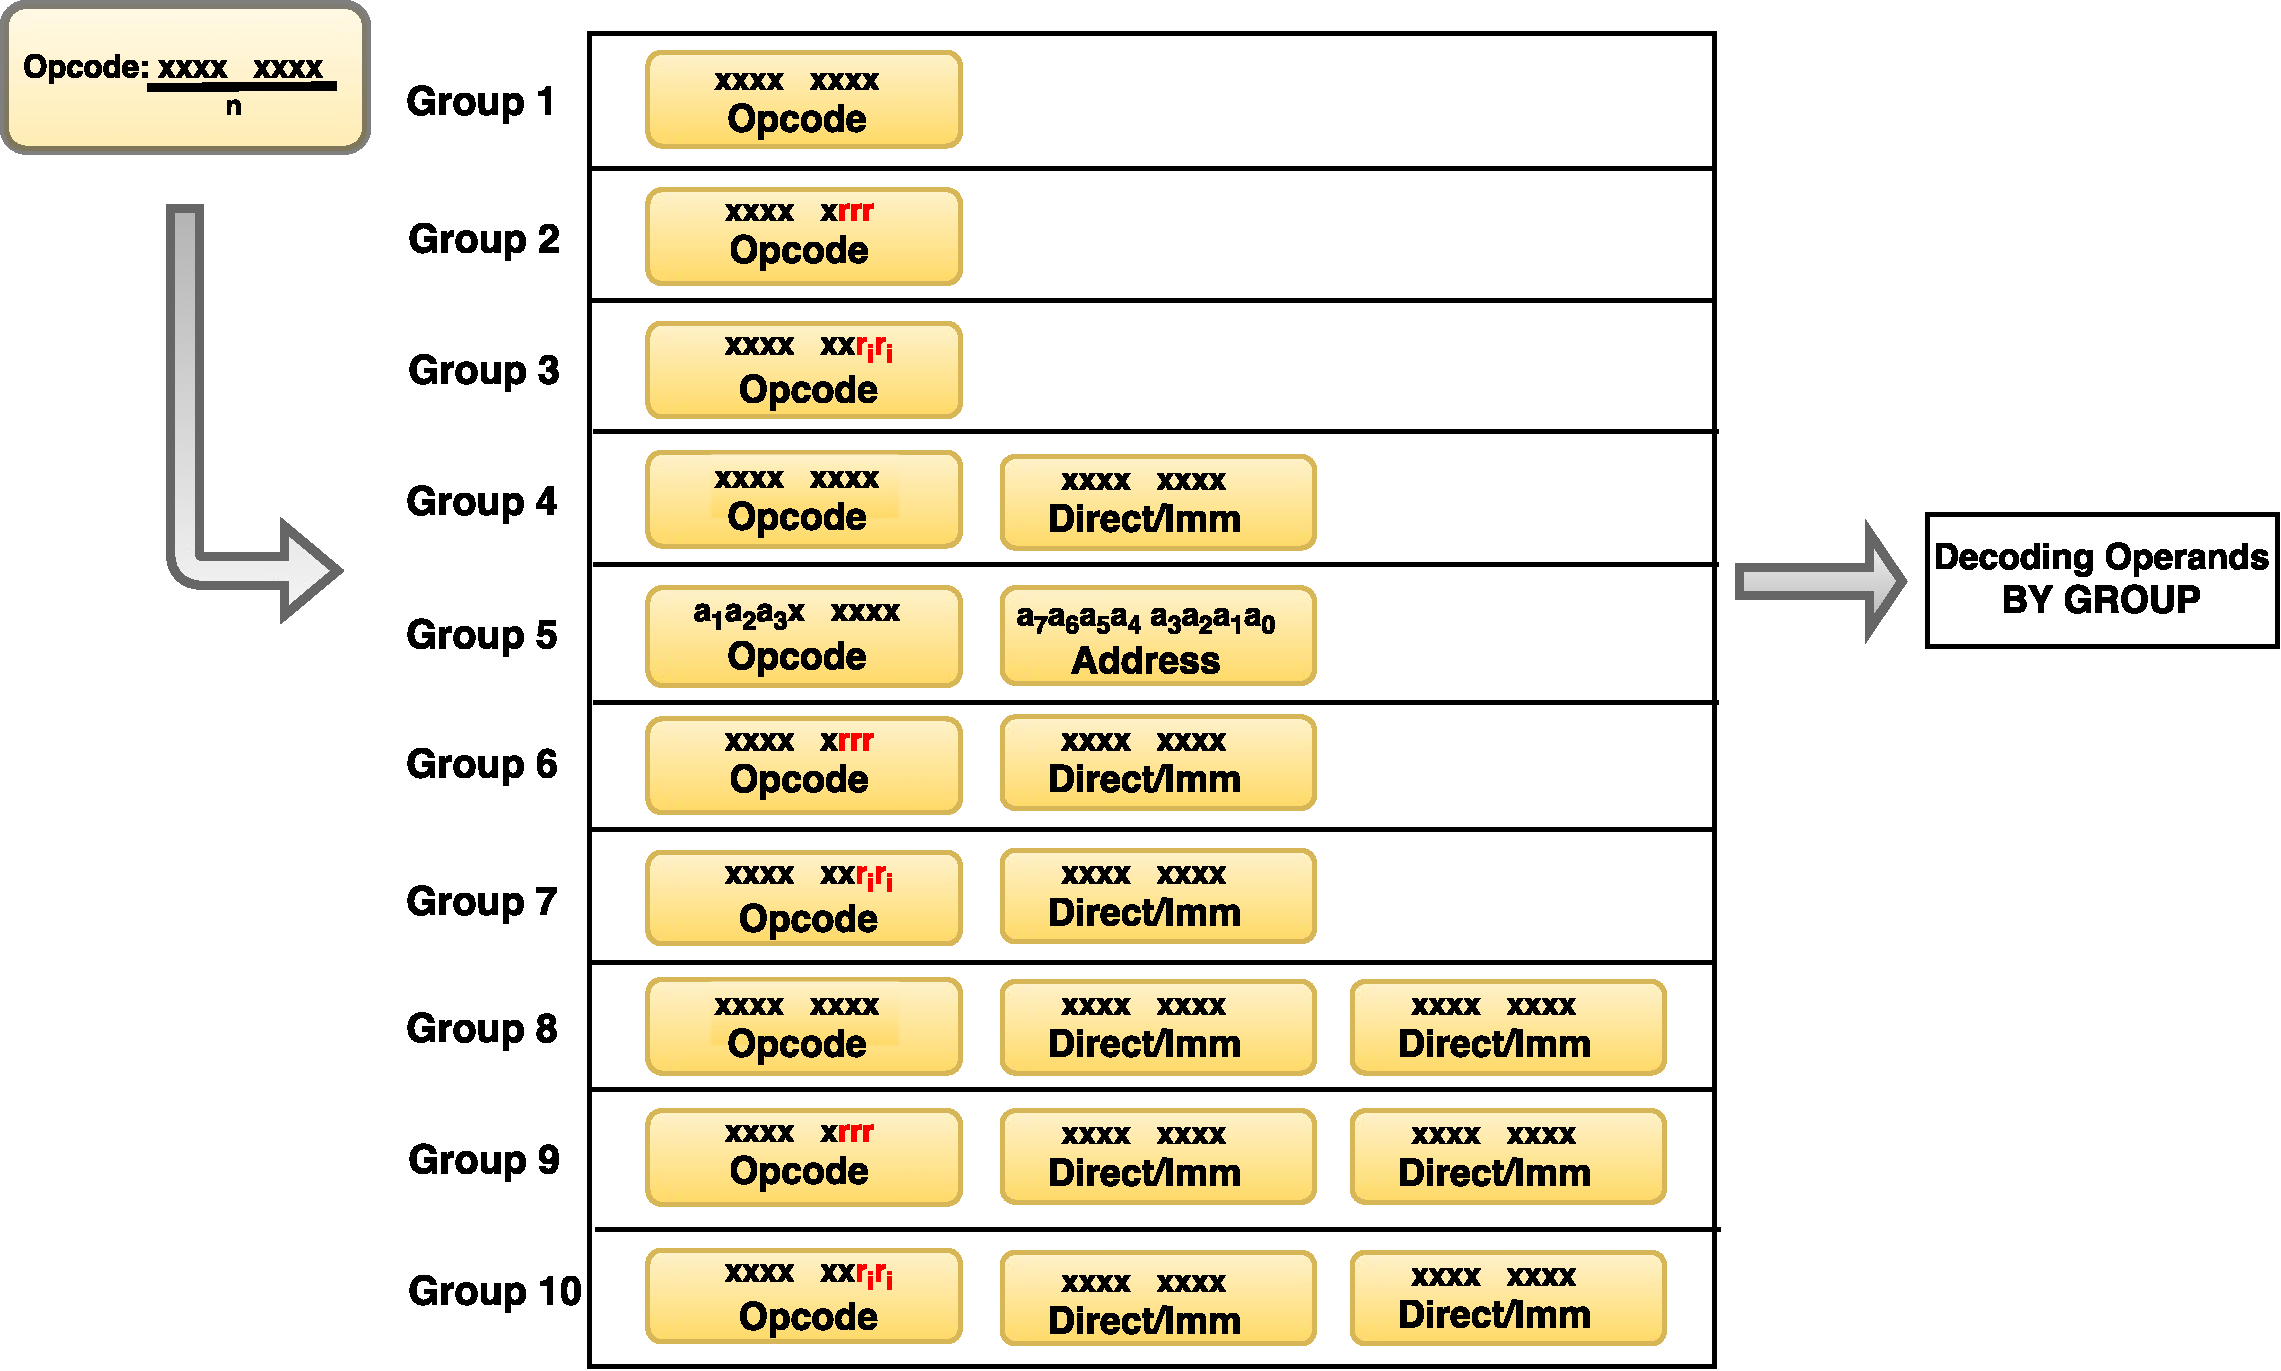
\includegraphics[scale=0.4]{images/Decoders_Behaviors3}
    }
    \caption{Decoder's Instruction Format behavior.}
    \label{fig:Decoders_Behavior3} 
    \end{figure}
	
    This type of decoder is also not implemented. Therefore, in order to achieve that gold, and since its behavior is based on the format of the instructions, there was also the need to check each instruction, evaluate it and according to its format, put it in the specif group. At the end, the result was the existence of 10 groups with the corresponding instruction format, as shown in figure \ref{fig:Decoders_Behavior3}. 
	Having the definition of the groups, the process is quite trivial. Basically, the opcode is acquired, and accordingly with its group, the operands are obtained. Due the selection of the group and other actions that must be executed, this behavior can cost a big price with a software implementation and can become a disadvantage. So, theoretically, a good alternative can be an hardware implementation. However, this implementation requires a different interface in the model (since the target instructions are created without intermediate representation using the operands obtained from the source instruction). For that, an appropriate (and additional) implementation in the generator shall be obtained to accomplish this approach. 

\subsubsection{Translation Cache Behavior}
% State: To Do 
\input{text/PD_ImplementationTechniques}

\subsubsubsection{Software Implementation - Hash Table}
% State: To Do 
As said before the translation cache can have multiple implementations, one of them is using a hash table format to manage the storage of more than one basic block. 

\begin{figure} [h!]
	\centering
	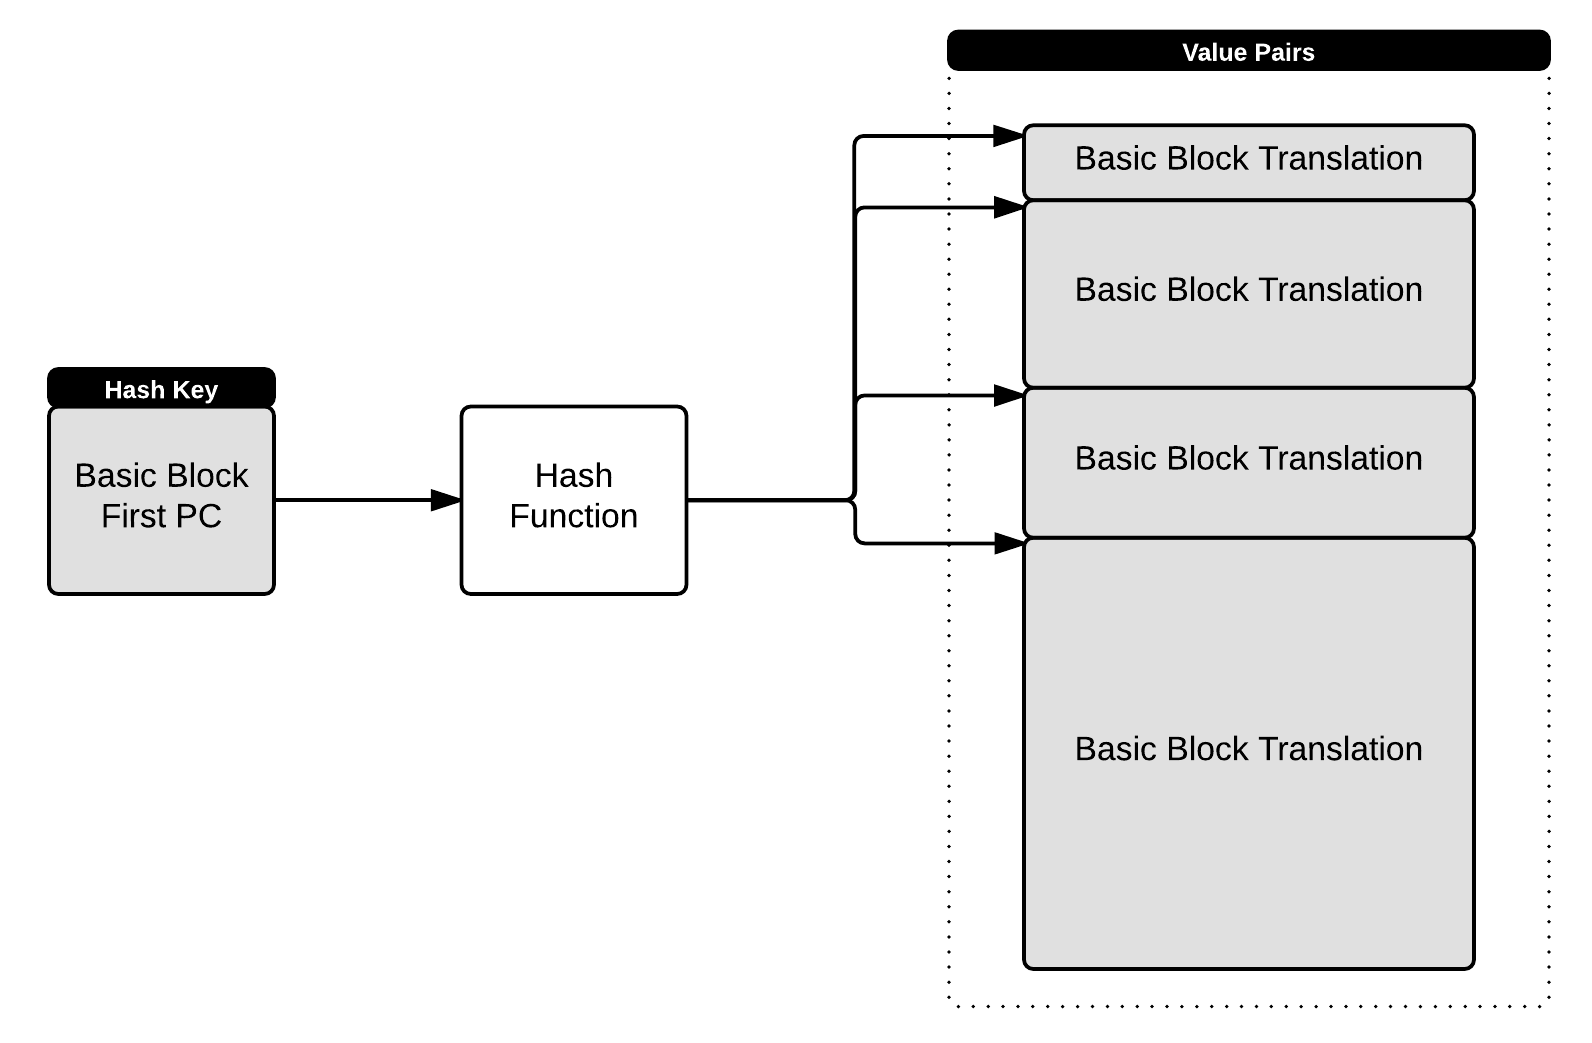
\includegraphics[scale = 0.2]{images/Hash.png}
	\caption{Mechanism for the hash table management.}
	\label{fig:Hash}
\end{figure}

This implementation has to respect the translation cache interface and so the following functions need to be implemented:
\begin{itemize}
	\item addtag - adds a new element to the list of basic blocks. We need to save the initial PC of the basic block that is passed as argument, the starting address of the basic block in the translation cache is equal to the address of the previous basic block plus the size of the previous basic block, and the size of the new basic block is set to zero.
	\item gettransaddr - this function receives a PC and compares it to the initial PC from each element in the basic block list and if there is a hit, the starting address of the corresponding basic block is returned.
	\item cachecode - this function is used to write in the translation cache. Two function need to be implemented, one to write one word, and one to write two words in the translation cache. To perform a write operation, we first need to check if there is enough room left for what we want to write. If there isn't, it is necessary to remove the oldest basic block in cache. But, even if there is room in the cache, another verification is needed. It's necessary to check if the basic block address plus the basic block size plus the new code size is bigger than the memory size. This means that we are in the end of the translation cache and the space that is available is in the beginning of the cache. When this happens we need to copy the basic block to the memory beginning and only then perform the write operation. To do this it's necessary to make room in the memory beginning to copy the entire basic block.
\end{itemize}


\subsubsubsection{Hardware Implementation}
% State: To Do 
The translation cache implementation in software is one of the most time-critical processes in the Dynamic Binary Translator. To improve this process, we will use the technique of \textbf{hardware offloading} in order to implement the Translation Cache in hardware. 
The goal of the hardware implementation is to speed up the process of finding if a basic block is already translated and where it is translated, and, by searching in parallel, this can be achieved in one clock cycle. The write operation can also be speed up by performing all cache management in hardware.

There are two similar ways to implement the TCache in hardware. The first is to implement all the Translation Cache in hardware. The second is to implement only the logic unit of the TCache in hardware, which is a Content Addressable Memory. The main difference between them is:
\begin{itemize}
	\item Translation Cache (CAM and RAM) - Stores the translated Basic Blocks in the RAM, which is a AXI peripheral too;
	\item CAM - Leaves the process of storing the translated Basic Blocks to the software.
\end{itemize}


\paragraph{TCache}
\paragraph{}

% State: To Do 
\begin{figure} [H]
	\centering
	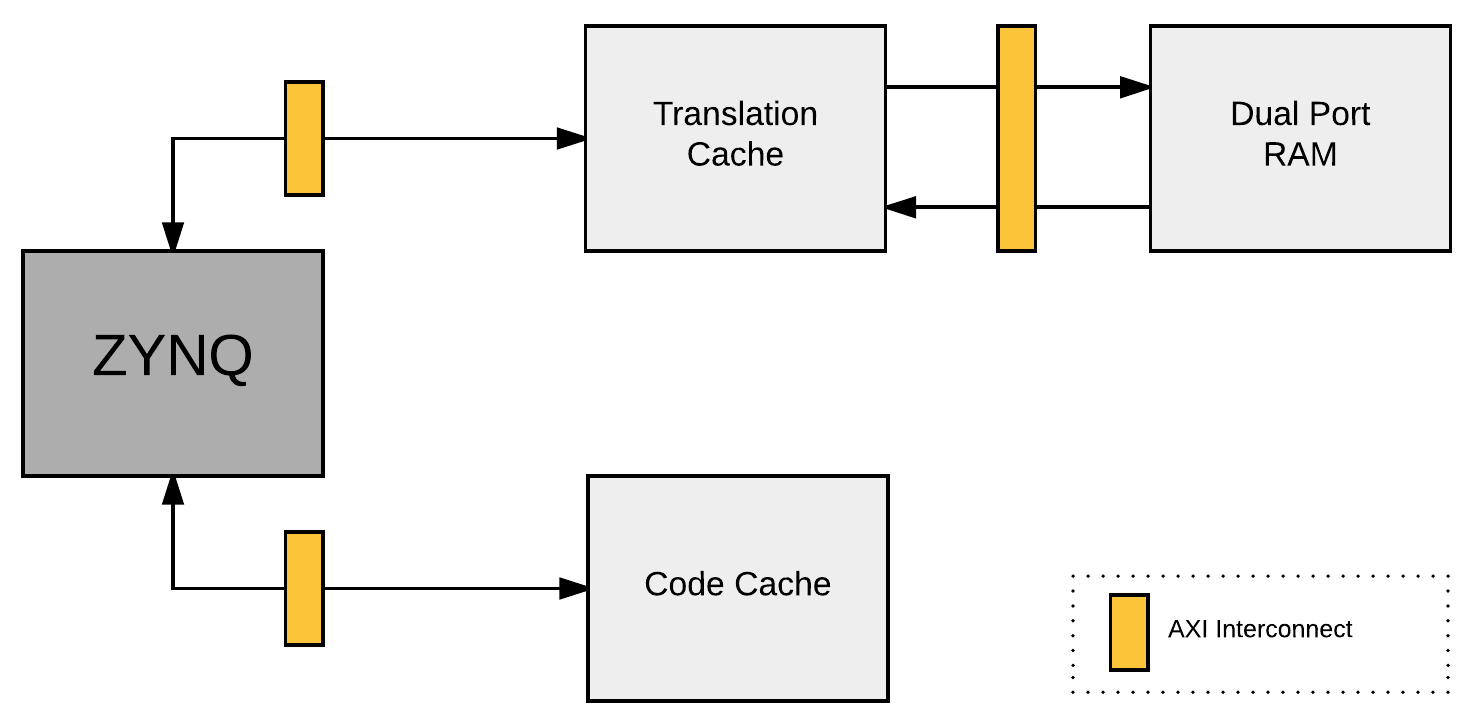
\includegraphics[scale = 0.2]{images/DesignHw1.png}
	\caption{Translation Cache hardware implementation with AXI Protocol}
	\label{fig:TCache_Hw}
\end{figure}

The first is represented in the figure \ref{fig:TCache_Hw} and probably less efficient is to create two AXI peripherals:
\begin{itemize}
	\item Translation Cache - Implemented AXI LITE peripheral;
	\item Dual Port RAM - Includes a BRAM Controller and a Block Memory Generator, both provided by Xilinx.	
\end{itemize}

For this implementation, the \textit{TCache} peripheral instantiate a CAM Module in order to find if the actual BB is or isn't translated and to return the address in the RAM where is the translation;

\paragraph{CAM}
\paragraph{}

% State: To Do 
\begin{figure} [H]
	\centering
	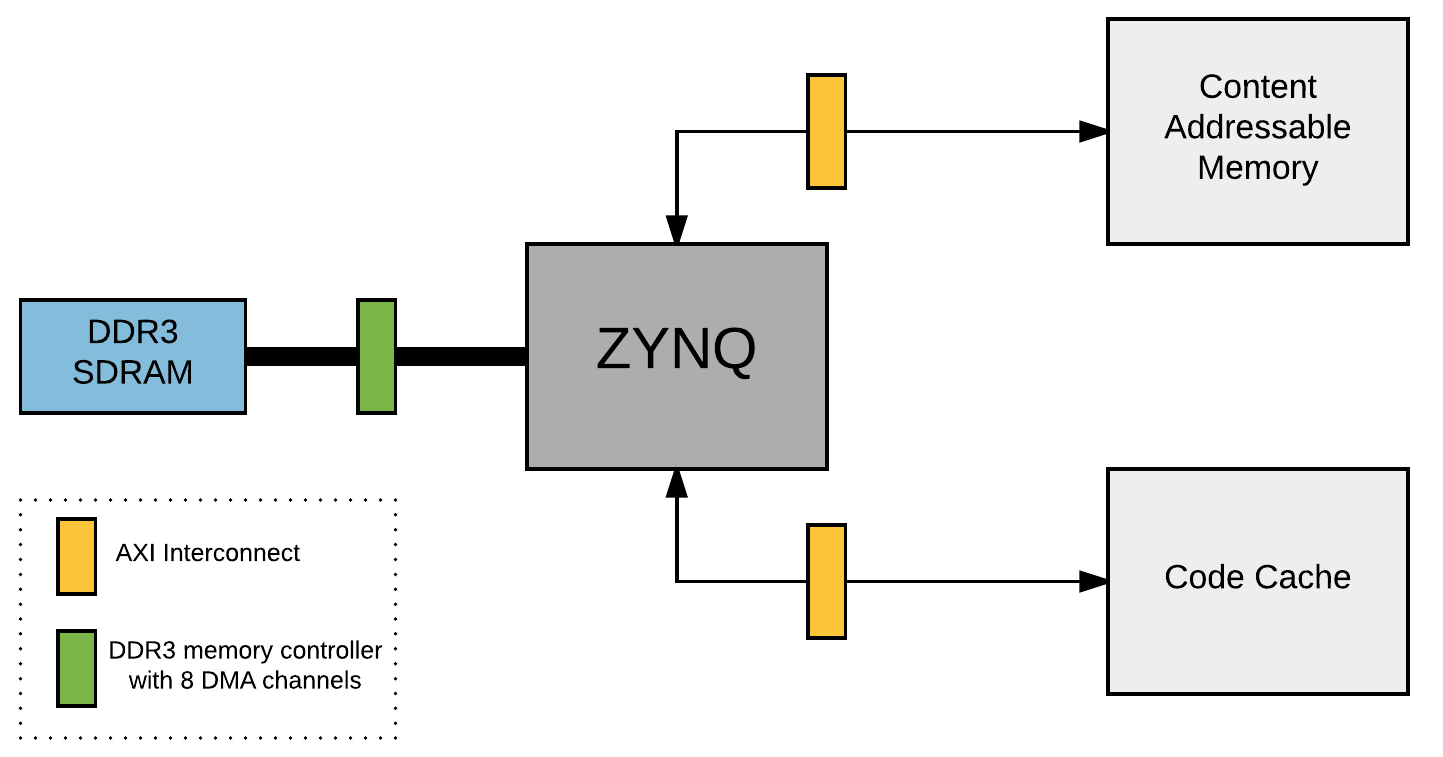
\includegraphics[scale = 0.2]{images/DesignHw2.png}
	\caption{Content Addressable Memory hardware implementation with AXI Protocol}
	\label{fig:CAM_Hw}
\end{figure}

The second way is represented in the figure \ref{fig:CAM_Hw} and is probably the most efficient way is to implement only a Content Addressable Memory, that allows to know the address where a word is located. 

For this implementation we need a table that contains the initial PC of each translated basic block and the address where it is translated, it also stores the basic block size for management necessities.

\begin{figure} [H]
	\centering
	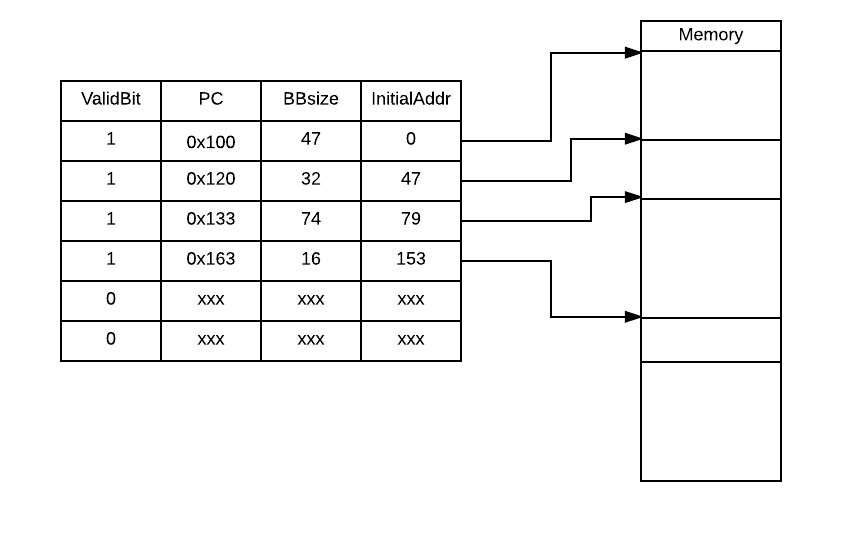
\includegraphics[scale = 0.35]{images/CAM.png}
	\caption{Content Addressable Memory Table}
	\label{fig:CAM_table}
\end{figure}

This implementation also needs to respect the same interface, and so whenever we want to add a new tag, we first check if the number of basic blocks is maxed out, and if so we remove the oldest. Then we add an entree to the table saving the initial PC of the basic block, and the address corresponding to it that is the address of the previous basic block plus the previous basic block size.

\begin{figure} [h!]
	\centering
	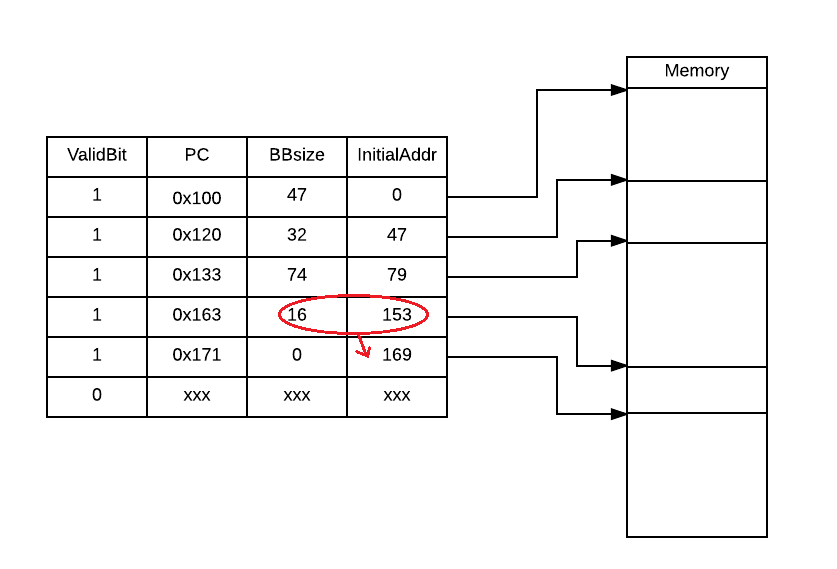
\includegraphics[scale = 0.35]{images/CAM_new_BB.png}
	\caption{Content Addressable Memory Table: starting new basic block translation}
	\label{fig:CAMtableNewBB}
\end{figure}

To know if a basic block is translated we simply need to search the table for the initial PC and if there is a hit return the address where it is translated.
To perform the write operation, first it is necessary to check if there is room in the memory for the new instruction and if there isn't the oldest basic block must be removed. To do this it is not necessary to delete the basic block from memory, it's only needed to remove a line from the CAM as all management is done by the CAM, the data in memory will be overwritten. It's necessary to check if the basic block address plus the basic block size plus the new code size is bigger than the memory size. This means that we are in the end of the translation cache and the space that is available is in the beginning of the cache. When this happens we need to copy the basic block to the memory beginning and only then perform the write operation. To do this it's necessary to make room in the memory beginning to copy the entire basic block.




\subsection{Implementation Plan}
At this point, due to all the study and work done in the Analysis and Design phases, everything is quite well defined. Having said that, it was elaborated an implementation plan that will serve as an orientation and also as a kind of check list. Figure \ref{fig:implementation_plan} shows the implementation plan developed:

\begin{figure}[!htb]
\centerline{
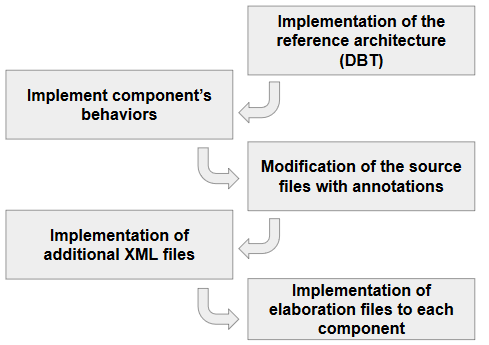
\includegraphics[scale=0.75]{images/Implementation_Plan.png}
}
\caption{Implementation Plan Diagram}
\label{fig:implementation_plan} 
\end{figure}

First of all, the groups that are committed to the DBT will implement the reference architecture using the EL language. In an initial phase, the team shall work together and discuss some common issues. Then, each group shall work independently until the global integration. 

Some component's behaviors are not implemented and some only have one behavior which are already implemented. For example, all the decoder's behaviors explained before shall be implemented, some in hardware, some in software and some in both. The first decode based in switch cases is already implemented in the DBT. By so, only an elaboration file will be created for it. The second decode based in jump tables shall have two possible implementations: one only in software and another with some management implemented in hardware. The idea behind that is to prove the concept that two elaboration files can be created without changing the model. Also, if proved, this approach will perform accelerations in the system. However, the DBT system must be ported into an FPGA system, in this case, the Zybo Board referred in the analysis section. So, this task must also be taken. Finally, the last type of decoder (Instruction Format) will be implemented in hardware, however, will not be tested since its required a new behavior for the generator component. 

With the sources prepared, what comes next is the modification of the source files with annotations in the right locations and the creation of the elaboration files for all components of the model. Since some component's behaviors have specific parameters, additional XML files for them must be implemented. 



\subsection{Test Cases}
To close an implementation and to ensure that everything were performed correctly, unit and global tests must be done. The diagram presented in figure \ref{fig:tests} reveal the kind of tests that must be validated. 

\begin{figure}[H]
\centerline{
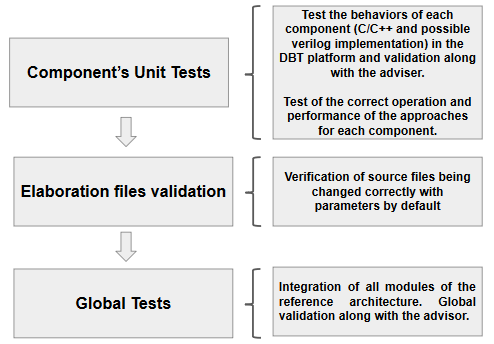
\includegraphics[scale=0.8]{images/TestCases.png}
}
\caption{Tests Diagram}
\label{fig:tests} 
\end{figure}

Since one of the goals is to implement the different components behaviors, a test to each implementation should be accomplished. If the result is positive, then the integration  of the decode in the DBT is made. Also, performance tests are a goal because it will allow to conclude which behaviors are more efficient. Regarding the implementations in hardware, the group hopes to test those implementations in the Zybo board.

Being the components implementations approved, it is verified if the elaboration files of each component replace the annotations in the sources files correctly, meaning that it is checked if the final source files are generated properly.

In the end, all the modules of the DBT will be integrated and a bunch of tests with different configurations will be done.

%%%%%%%%%%%%%%%%%%%%%%%%%%%%%%%%%%%%%%%%%%%%%%%%%%%%%%%%%%%%%%%%%%%%%%%%%%%%%%%%%%
%  IMPLEMENTATION / TEST UNIT
%%%%%%%%%%%%%%%%%%%%%%%%%%%%%%%%%%%%%%%%%%%%%%%%%%%%%%%%%%%%%%%%%%%%%%%%%%%%%%%%%%

\newpage
\section{Implementation and Unit Testing}


\subsection{Code Refactoring}
In the design phase, the original code of the DBT system was analyzed. In order to obtain a system with modules directly related with the source code and to improve its internal structure, the refactoring process was performed over the original DBT system. This section describes the main modifications and the structure of the final system. 


\subsubsection*{CBuffer and CTransBuffer}

\textbf{CCache} and \textbf{TCache} are two atomic subcomponents of the DBT. In the original source code, they are represented in two classes: \texttt{CBuffer} and \texttt{TBuffer}. Since these classes only define services, there was no need for modifications of the source files.

\begin{figure}[H]
\centerline{
\includegraphics[scale=0.5]{images/Refactor_caches}
}
\caption{CBuffer and CTransBuffer UML diagram.}
\label{fig:refactorcaches} 
\end{figure}


\subsubsection*{CSourceArchitecture and C8051Arch}

Since the \textbf{Source Cluster} is one of the main components of the \textit{DBT}, an arrangement in the original source code was made in order to associate its subcomponents: \textbf{Source Architecture}, \textbf{Decoder} and \textbf{SourceEnvironment}. 

Respecting the reference architecture, a base class called \texttt{CSourceArchitecture} was created in order to encapsulate the abstract behavior of the Source Cluster related to all of its subcomponents. The class members were defined accordingly with the interaction presented in the DBT model. Those members are:
\begin{itemize}
\item An object of type \texttt{CBuffer}, which stores source code and has services used by the source cluster components (\textbf{composition} association).
\item An object of type \texttt{SourceEnvironment}, represented in the model as SourceEnvironment component (\textbf{composition} association).
\item A pointer to the class \texttt{CTargetArchitecture}, allowing the subcomponents of the source cluster to reference services provided by the components defined the target cluster (\textbf{aggregation} association).
\item Pointers to internal variables declared in \texttt{CDBTEngine} (explained latter) such as \texttt{eoBB, eoExec} and \texttt{SourcePMem} since those belong to an interface declared as a service in the DBTEngine component.
\item A virtual method called \texttt{decode} with the same role as in the original code.
\end{itemize} 

The base class was created in order to allow the redefinition of a specific source architecture in a easy way. By so, a concrete class named \texttt{C8051Arch} was implemented, which derives from \texttt{CSourceArchitecture} and implements all specific behavior. Thus, the \texttt{decode} method was overloaded (virtual function) and additional methods were added (\texttt{fineDecode0x0, fineDecode0x1}, ...) to perform the decode procedure. Anytime a designer intends to change the source architecture, a similar class must be created and derived from the referred base class. In this way, all interfaces are respected since it inherits all methods and variables.

\begin{figure}[!htb]
\centerline{
\includegraphics[scale=0.53]{images/Refactor_src}
}
\caption{CSourceArchiecture and C8051Arch UML diagram.}
\label{fig:sourcearchitectureUML} 
\end{figure}



\subsubsection*{CTargetArchitecture and CCortexM3}

The idea behind the Source Cluster class representation in the project is the same as the \textbf{Target Cluster}. This components is composed by two components: \textbf{TargetArchitecture} and \textbf{Generator}. A base class was created, called \texttt{CTargetArchitecture}, which has the abstract behavior of the Target Cluster component. This class defines all variables and methods that must be overloaded by a specific target architecture class, in order to respect the interfaces established in the model.  The basic class is composed by the following members:

\begin{itemize}
\item An object of type \texttt{CTransBuffer}, which stores translated code and has methods used by the target cluster components (\textbf{composition} association).
\item A pointer to an object of type \texttt{SourceEnvironment} (\textbf{aggregation} association), since the Generator component references services provided by this class.
\item A pointer to an internal variable of the \texttt{DBTEngine} class, \texttt{eoBB}, referenced also by the Generator.
\item Generic virtual methods (\texttt{gen\_X} functions) used to implement the target code generation. 
\end{itemize}

\begin{figure}[H]
\centerline{
\includegraphics[scale=0.5]{images/Refactor_trg}
}
\caption{CTargetArchitecture and CCortexM3 UML Diagram}
\label{fig:refactortrg} 
\end{figure}


Like \texttt{C8051Arch}, a concrete class for a specific target architecture must be derived from the base class \texttt{CTargetArchitecture}, in order to implement the specific behavior for the generator component. 


\subsubsection*{CDBTEngine}

The final structural modification was done to add another class to the project: \texttt{CDBTEngine}. This class encapsulates the engine of the DBT, namely, the process of translation of source code stored in \texttt{CBuffer} and execution of native code stored in \texttt{CTransBuffer}. 

The class contains the following variables and function members:
\begin{itemize}
\item Two objects of type \texttt{C8051Arch} and \texttt{CCortexM3} (\textbf{composition}), each one providing services from each cluster.
\item Several variables such as \texttt{eoExec, eoBB, SourcePMem, exit\_addr and sourceProgSize}, all used in internally in the engine.
\item A method used for the initialization of the DBT (\texttt{initTranslator}) and another for running (\texttt{runDBT}).
\item Two methods identified as components in the model: \texttt{execute} and \texttt{translate}.
\end{itemize}


\begin{figure}[H]
\centerline{
\includegraphics[scale=0.6]{images/Refactor_DBTEngine}
}
\caption{CDBTEngine UML diagram.}
\label{fig:refactorproject} 
\end{figure}


\subsubsection*{Project Sources and Headers}

Given the fact that new classes were added and others deleted, the organization of the final project sources was different form the original. New source files were added to encapsulate the new classes and new headers were created to have all definitions organized by their type.

Figure \ref{fig:refactorunderstand} shows a dependency graph created using the framework \textit{Understand™}, containing the source files of the DBT organized by subcomponents (\textbf{Target Cluster, Source Cluster, TCache, CCache} and \textbf{DBTEngine}).
 
\begin{figure}[!htb]
\centerline{
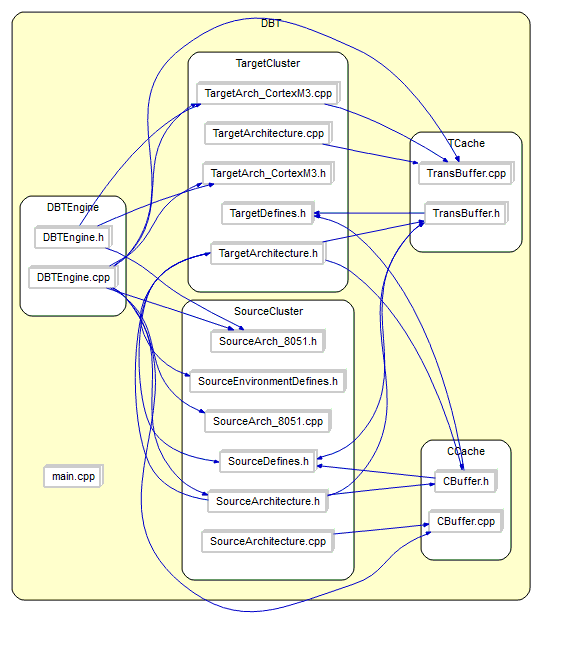
\includegraphics[scale=0.7]{images/DBT_understand}
}
\caption{Dependency graph of the DBT project files.}
\label{fig:refactorunderstand} 
\end{figure}

The dependencies observed were created using \textbf{calls} and \textbf{imports}. It becomes evident the relationship between the code of the project and the model created for the DBT. Comparing figure \ref{fig:refactorunderstand} (new version) with figure \ref{fig:understand} (old version), it is possible to see that:
\begin{itemize}
\item Four files were deleted (\texttt{Translate.cpp, Translate.h, Translate8051.cpp} and \texttt{Translate8051.h}.
\item Six files were added related with the source architecture (\texttt{SourceArchitecture.cpp}, \texttt{SourceArchitecture.h}, \texttt{SourceArch\_8051.cpp}, \texttt{SourceArch\_8051.h}, \texttt{SourceEnvironmentDefines.h} and \texttt{SourceDefines.h}).
\item Five files were added related with the target architecture (\texttt{TargetArchitecture.cpp}, \texttt{TargetArchietcture.h}, \texttt{TargetDefines.h}, \texttt{TargetArch\_CortexM3.cpp} and \texttt{TargetArch\_CortexM3.h}).
\item Two files were added containing the DBT engine (\texttt{DBTEngine.cpp} and \texttt{DBTEngine.h})
\end{itemize}

The referred files contain the classes that were created. However, there are two new headers that are composed by definitions of both architectures: \texttt{SourceDefines.h} and \texttt{TargetDefines.h}. These files are deeply related with the services provided by the architectures components of the model, i.e., the name of the registers, the size of the memories, the size of the word, among others. 

\subsection{Behaviors}
\subsubsection{Decoder Behaviors}
As it was referred in the \textit{Implementation Plan},  the group committed to implement 4 behaviors for the decoder component. Some of the behaviors were implemented in software, using C++ language, and some implemented adopting some management in hardware, using verilog. The behaviors implemented were:

\begin{itemize}
	\item \textbf{Switch Cases} Decoder (\textit{Sw}).
    \item \textbf{Jump Table} Decoder (\textit{Sw}/\textit{Hw}).
    \item \textbf{Generic} Decoder (\textit{Sw}).
    \item \textbf{Instruction Format} Decoder (\textit{Hw}).
\end{itemize}

In the following sections it will be presented each behavior implemented, along with some relevant code examples and unit tests to prove the proper functioning.


\subsubsection{Switch Cases}
The principle of operation is based on \textbf{switch cases}.
The original decoder behavior, present in the reference \textit{DBT}, is also based in switch cases but has always the \textbf{same number of cases per switch case} (listing \ref{lst:old_switchcases}).

\begin{lstlisting} [language=C++, caption=Original Switch Cases Behavior (first switch case)., label=lst:old_switchcases]
void CTranslator8051::decode(uint8_t op){
			uint8_t subOp = op & 0x0F;
			uint8_t regN = op & 0x7;	

			switch(op>>4){
					case 0 :
						fineDecode_0x0(subOp, regN);	break;
					case 1 :
						fineDecode_0x1(subOp, regN);	break; 
     ...   
\end{lstlisting}

For each \texttt{fineDecode\_0x...()} function another switch case is present inside and in each of its cases relies the decoding algorithm for each instruction (listing \ref{lst:old_switchcases2}). Since it is always being used the 4 most significant bits of the opcode for the first switch case and the other 4 bits for the switch cases inside each \texttt{fineDecode\_0x...()} function, the max size of the switchs will be $2^{4}$. So, there are $2^{4}$ \texttt{fineDecode\_0x...()} methods defined.

\begin{lstlisting} [language=C++, caption=Original Switch Cases Behavior (portion of the \texttt{fineDecode\_0x0()} function)., label=lst:old_switchcases2]

void CTranslator8051::fineDecode_0x0(uint8_t subOp, uint8_t Rn)
{
			uint8_t tmp1;
			uint16_t newPC;
		
			switch (subOp) {
					case 0: //NOP
							zprintf("\tNOP\n\n");
	  	break;
					case 1: // AJMP
							tmp1 = FETCH;
							newPC = (env.PC & 0xF800) | 0x0000 | (uint16_t)tmp1; 
	    				gen_writePC(newPC);		
	    				zprintf("\tAJMP 0x%04X\n\n", newPC);
							eoBB = true;		
			break;
		
    ...

\end{lstlisting}

For the new implementation, the idea remains the same, but now it is given the possibility to \textbf{choose the number of bits of the opcode for the evaluation in the switch cases} (point configurable by the user). This way, a more generic approach had to be taken and it will be demonstrated next.

\subsubsubsection{Software Implementation}

  In order to ensure a dynamic size for the switch cases what was done was define 256 callback functions ($2^{nBitsOpcode}$, being the nBitsOpcode = 8) to, independently of the user choices, in the end be always called the \texttt{finedecode\_0x...()} function according to the traversal along the switch cases (again, based on the opcode). Listing \ref{lst:new_switchcases} show the current aspect of some \texttt{fineDecode\_0x...()} functions.

\begin{lstlisting} [language=C++, caption=\texttt{fineDecode\_0xe7()} and \texttt{fineDecode\_0xe8()} functions., label=lst:new_switchcases]
void  C8051Arch::fineDecode_0xe7(uint8_t subOp, uint8_t Rn)	// MOV A, @Ri
{   
			target->gen_ld8(tReg2, subOp&0x01 );
  		target->gen_ldi8(tReg1, MEM_BASE, tReg2);
			target->gen_st8(A, tReg1);
			zprintf("\tMOV A, @R%d\n\n", subOp&0x01);  
} 

void  C8051Arch::fineDecode_0xe8(uint8_t subOp, uint8_t Rn)	// MOV A, Rn
{   
			target->gen_ld8(tReg1, Rn); // Load Rn.
			target->gen_st8(A, tReg1);  // Store the value to A.
			zprintf("\tMOV A, R%d\n\n", Rn); 
}
\end{lstlisting}

Now, as it can be seen, the algorithm to decode a specific instruction is inside the respective \texttt{fineDecode\_0x...()} function. So, for example, the instruction whose opcode equals \texttt{0xe8} will "fall" into the \texttt{fineDecode\_0xe8()} callback. Listing \ref{lst:new_switchcases2} shows a portion of the aspect of the switch cases. For the first one is used 7 bits (\texttt{range1}) and for the others 1 bit (\texttt{range2}).

\begin{lstlisting} [language=C++, caption=Portion of the decode function using the Switch Cases behavior., label=lst:new_switchcases2]
void C8051Arch::decode()
{
			uint8_t op = FETCH;
			uint8_t subOp = op & 0x0F;
			uint8_t regN = op & 0x7;
	
			uint8_t range1 = (op >> 1), range2 = (op & 0x1);

			switch  (range1) {
			case 0x0:
	  			switch (range2) {
	  					case 0x0:
	    					fineDecode_0x0(subOp, regN);
	    				break;
	  					case 0x1:
	    					fineDecode_0x1(subOp, regN);
	   					break;
	  			}
			break;
			case 0x1:
	  			switch (range2) {
	  					case 0x0:
	    					fineDecode_0x2(subOp, regN);
	    				break;
	  					case 0x1:
	    					fineDecode_0x3(subOp, regN);
	    				break;
	  			}
			break;
            
	  ...
\end{lstlisting}

Since for the \texttt{range2} is only used the least significant bit of the opcode, the secondary switch cases have only two cases (0 or 1).	 

\subsubsubsection{Unit Tests}

In order to test the implemented decoder, a simple test will be presented showing its correct functioning. A basic block was created and stored in memory and the output of the system was logged. This procedure was repeated for several basic block, however, only one example is presented in \ref{fig:teste1_decoder}.   


\begin{figure}[H]
\centerline{
\includegraphics[scale=0.5]{images/teste_decoder1}
}
\caption{Decoder 1 - Unit Test.}
\label{fig:teste1_decoder} 
\end{figure}

As shown, the output was as expected. All instruction that compose the basic block were translated accordingly. The basic block ends in a branch instruction (SJMP).

\subsubsection{Jump Table}

Recalling the principle of operation of this type of decoder, it consist in an \textbf{array (table) of pointers to functions} that know how to decode a specific instruction. The opcode serves as index for the table, i.e., if an opcode equals \texttt{0x54}, it will be executed the function whose address is in the position \texttt{0x54} of the table. 


For this decoder behavior, an implementation in \textbf{software}(\textbf{\textit{Sw}}) and one in \textbf{hardware}(\textit{\textbf{Hw}}) was accomplished. Independently of the approach, the \textbf{256 callback functions} ($2^{nBitsOpcode}$, being the nBitsOpcode = 8) were defined. Those callback functions are the same as the ones referred in the Switch Cases decoder, the \texttt{fineDecode\_0x...()} whose job is, once again, take care of a specif instruction. So, the table will contain the addresses of this functions. 

In the hardware approach for this decoder, the behavior its not totally in hardware. The hardware is only a support to theoretically accelerate the process of decode. It will get clear later, in the hardware implementation section.

\subsubsubsection{Software Implementation}

Having in mind the idea of the decoder, what was necessary to do first was declare an array (table) of pointers to functions and a typedef as an alias for the pointer. Being \texttt{fineDecode} declared, 256 memory positions of the table were allocated dynamically (listing \ref{lst:jmptable1}). 

\begin{lstlisting} [language=C++, caption= \texttt{JmpTable} declaration, label=lst:jmptable1]
typedef void (C8051Arch::*fineDecode)(uint8_t, uint8_t);
		...
fineDecode *JmpTable;
		...
JmpTable = new fineDecode[NUM_Instructions];
\end{lstlisting}


It was created a new function to initialize the table. So, in the \texttt{initJumpTable()} function, the \texttt{JmpTable} array is filled with the addresses of each \texttt{fineDecode\_0x...()} function. It is possible to visualize a fragment of the function in listing \ref{lst:jmptable2}.   

\begin{lstlisting} [language=C++, caption= \texttt{initJumpTable()} function., label=lst:jmptable2]
void C8051Arch::initJumpTable(){

    JmpTable[0] = &C8051Arch::fineDecode_0x0;
    JmpTable[1] = &C8051Arch::fineDecode_0x1;
    JmpTable[2] = &C8051Arch::fineDecode_0x2;
    JmpTable[3] = &C8051Arch::fineDecode_0x3;
    JmpTable[4] = &C8051Arch::fineDecode_0x4;
    JmpTable[5] = &C8051Arch::fineDecode_0x5;
    JmpTable[6] = &C8051Arch::fineDecode_0x6;
    JmpTable[7] = &C8051Arch::fineDecode_0x7;
    JmpTable[8] = &C8051Arch::fineDecode_0x8;
    JmpTable[9] = &C8051Arch::fineDecode_0x9;
    JmpTable[10] = &C8051Arch::fineDecode_0xa;
    
    ...
\end{lstlisting}

Finally, using the opcode it is possible to access the correct position in the array and execute the respective \texttt{fineDecode\_0x...()} function (listing \ref{lst:jmptable3}).

\begin{lstlisting} [language=C++, caption=Callback function call (\texttt{decode} method)., label=lst:jmptable3]
(this->*(JmpTable[op]))(subOp, regN);
\end{lstlisting}

\subsubsubsection{Software Unit Tests}
A unit test was design to validate the jump table implemented in software. It is based in the previous unit test. Figure \ref{fig:teste1_decoder2} shows one basic block being translated.

\begin{figure}[H]
\centerline{
\includegraphics[scale=0.5]{images/teste_decoder2}
}
\caption{Decoder 2 - Unit Test.}
\label{fig:teste1_decoder2} 
\end{figure}

In the example, the basic block ends with a branch instruction (ACALL). In the same way, a set of basic blocks were loaded in memory in order to check if the translation occurs as expected for all cases. 

\subsubsubsection{Hardware Implementation}

As mentioned, this hardware implementation serves \textbf{as support} for the software. The only thing that is done in hardware is, after receive the opcode from the software, access to a specific register and \textbf{return} to the software \textbf{the function address to be executed}. This way, it is required to in a first prime, fill an array of registers in the hardware with the \texttt{fineDecode\_0x...()} addresses. The synchronization between the software and the hardware is ensured by means of signals using bits of registers. Also the exchanged data is made through registers. For the \textit{Sw} <-> \textit{Hw} communication, it is used the \textit{AXI} bus.

As it can be seen in listing \ref{lst:hw_jumptable} an \textbf{hardware jump table}, consisting in an array of 256 registers with 32 bits(function address size) each, was created and at every reset event the jump is clean, i.e, filled with zeros (listing \ref{lst:hw_jumptable2}).

\begin{lstlisting} [language=Verilog, caption=Hardware Jump Table., label=lst:hw_jumptable]
reg [`FUNC_SIZE-1 : 0] jmp_table [0 : `TABLE_SIZE-1];
\end{lstlisting}

\begin{lstlisting} [language=Verilog,caption=Jump Table initialization, label=lst:hw_jumptable2]
if(S_AXI_ARESETN == 1'b0)
begin
			for( i = 0 ; i < `TABLE_SIZE ; i = i + 1)
						jmp_table[i] <= 32'h00000000;

			init <= 1'b1;
			index <= 0;         
end
\end{lstlisting}

The software writes the function addresses, one at a time, in a register (\texttt{slv\_reg0}), signals (using the bit 9 of the \texttt{slv\_reg1} in listing \ref{lst:hw_jumptable3}) the hardware and the address stored in the hardware jump table.

\begin{lstlisting} [language=Verilog, caption=Jump Table initialization., label=lst:hw_jumptable3]
if(init == 1'b1 && slv_reg1[9] == 1'b1)
begin
      jmp_table[index] = slv_reg0;
      index = index + 1;
      init <= 1'b0; 
end
\end{lstlisting}

At decode time, the hardware receives the opcode, goes directly to the correct position of the \texttt{jmp\_table} array, writes the address in a register(\texttt{slv\_reg2}) and signals the software to read that register.

\begin{lstlisting} [language=Verilog, caption=Getting the function address., label=lst:hw_jumptable4]
slv_reg2 = jmp_table[slv_reg1[`OPCODE]];

...


if(slv_reg1[8] == 1'b1)
begin           
		slv_reg3 <= 1; 
end
end
\end{lstlisting}

\subsubsubsection{Hardware Unit Tests}

To test this hardware implementation, it was used the Vivado environment. So, a testbench was created and it was simulated a request from the software, i.e., simulate a request to obtain a certain function address that is in the hardware register array (table). But first, it was necessary to fill the table and, to make the test easier, the content of each register of the array got the number of the index (simulated function addresses = index of the array).

\begin{figure}[H]
\centerline{
\includegraphics[scale=0.5]{images/test_bench}
}
\caption{Decoder 2 - Hardware Unit Test.}
\label{fig:test_bench} 
\end{figure}

As it can be seen in the figure \ref{fig:test_bench}, that in the red circle there is a simulated opcode (0x64). With that, it can be verified in the blue circle that the simulated function address is 0x64 (equals the index of its position) and the signal to the software (purple circle) is set. 
\subsubsection{Generic}

Another behavior proposed in the design phase as a new approach for a decode procedure consists in a generic version of the jump table. However, instead of having a table of callback functions, the table is composed by a structure with information about the steps that must be taken to achieve the target code generations (after decoding the operands).

\subsubsubsection{Software Implementation}

The first step in this approach was the definition of the structure. The main idea is to have a \textbf{table} that stores the functions used in the decode process and a \textbf{matrix} that stores references for internal variables used inside those functions. The referred structure is presented in listing \ref{lst:InstructionDecodeSteps}.

\begin{lstlisting} [language=C++, caption= InstructionDecodeSteps structure., label=lst:InstructionDecodeSteps]
typedef void* arg_P;
typedef void (C8051Arch::*method_P)(arg_P*);

struct InstructionDecodeSteps 
{
		method_P* steps;
    arg_P **auxVar;
    int numSteps;
    InstructionDecodeSteps(int numSteps, int numMaxArgs);
};
\end{lstlisting}

As shown, the structure contains a table of type \texttt{method\_P} (\textbf{steps}) and a matrix of type \texttt{arg\_P} (\texttt{auxVar}). The typedef \texttt{method\_P} defines a pointer to a member function of \texttt{C8051Arch} which receives only one argument. This arguments corresponds to a row of the matrix \texttt{auxVar} which contains references to auxiliary variables that shall be used (set/get) inside each method. The table of \texttt{InstructionDecodeSteps} structures with 256 positions were declared as follows:

\begin{lstlisting} [language=C++, caption= InstructionDecodeSteps table declaration., label=lst:generic_jmptable2]
InstructionDecodeSteps** JmpTable;
			...
JmpTable = new InstructionDecodeSteps*[NUM_Instructions];	
\end{lstlisting}

Finally, the table was filled inside the constructor of the class. For that, an exhausting analysis of the decoder code was done. In a generic way, each decode function is composed by a set of generation functions (\texttt{gen\_xx} functions) and auxiliary operations. Since the generation function are already implemented, only new functions were created to implement those operations. Listing \ref{lst:auxMethods} shows the auxiliary methods created.    

\begin{lstlisting} [language=C++, caption= Auxiliary methods, label=lst:auxMethods]
	void fetch(arg_P * ptr);
	void set_eoBB(arg_P * ptr);
	void set_eoExec(arg_P * ptr);
	void AuxFunc_NewPCx(arg_P * ptr);
	void AuxFunc_2bytes(arg_P * ptr);
	void AuxFunc_Ri(arg_P * ptr);
	void AuxFunc_Rn(arg_P * ptr);
	void AuxFunc_ByteAddrAssign(arg_P * ptr);
	void AuxFunc1_0x80(arg_P * ptr);
\end{lstlisting}

As expected, this implementations requires that all steps must have the same signature (one arguement of type \texttt{arg\_P*}). However, the generation functions don not follow this requirement. To overcome this problem, an arrangement was made and wrappers were created around these methods. This approach has a disadvantages since these wrappers increase the overhead. This can be avoided by rewriting every generation function of the target architecture.

\begin{lstlisting} [language=C++, caption = Generation functions., label=lst:gen_generic]
	void gen_movi_wrapper(arg_P * ptr);
	void gen_ld8_wrapper(arg_P * ptr);
	void gen_ldi8_wrapper(arg_P * ptr);
	void gen_st8_wrapper(arg_P * ptr);
	void gen_sti8_wrapper(arg_P * ptr);
  void gen_cje_wrapper(arg_P * ptr);
	void gen_cjne_wrapper(arg_P * ptr);
  
  ...
\end{lstlisting}

Having all methods created, the next step consists in fill all positions of the table. Listing \ref{lst:filltable} illustrates the procedure made for two instruction: \textbf{NOP} and \textbf{AJMP}.

\begin{lstlisting} [language=C++, caption= Initialization of table of structures.
, label=lst:filltable]
	
	// 0x00   NOP
	JmpTable[0x00] = new InstructionDecodeSteps(1, 0);
        JmpTable[0x00]->steps[0] = &C8051Arch::print_NOP;

	//0x01   AJMP
	JmpTable[0x01] = new InstructionDecodeSteps(5, 4);

	JmpTable[0x01]->steps[0] = &C8051Arch::fetch;   //1st step
	JmpTable[0x01]->auxVar[0][0] = &tmp1;           //auxvar1

	JmpTable[0x01]->steps[1] = &C8051Arch::AuxFunc_NewPCx;   //2nd step
	JmpTable[0x01]->auxVar[1][0] = &newPC;                   //auxvar2
	JmpTable[0x01]->auxVar[1][1] = (uint16_t *) &env.PC;     //Src PC
	JmpTable[0x01]->auxVar[1][2] = &v_0x0000;                // 0 
	JmpTable[0x01]->auxVar[1][3] = &tmp1;                    //auxvar1

	JmpTable[0x01]->steps[2] = &C8051Arch::gen_writePC_wrapper;  //3rd step
	JmpTable[0x01]->auxVar[2][0] = &newPC;                    //auxvar2

	JmpTable[0x01]->steps[3] = &C8051Arch::set_eoBB;      //4th step
	JmpTable[0x01]->auxVar[3][0] = (bool *)eoBB;          //eoBB
        
	JmpTable[0x01]->steps[4] = &C8051Arch::print_AJMP;   //5 step
	JmpTable[0x01]->auxVar[4][0] = &newPC;               //debug

	//0x02   LJMP
	
   ...
\end{lstlisting}

Finally, it is presented the decode method for this implementation (listing \ref{lst:decodetable}). Having all steps defined, the method consists in a simple loop through all positions of the step table. 

\begin{lstlisting} [language=C++, caption=Decode method for generic decode behavior.
, label=lst:decodetable]
void C8051Arch::decode()
{
		uint8_t op = FETCH;

    int i, nSteps; v_opcode = op;

    for( i = 0 ; i < JmpTable[op]->numSteps ; i++ )
    {
    	(this->*(JmpTable[op]->steps[i]))(JmpTable[op]->auxVar[i]);
    }      
		return;
}
\end{lstlisting}

\newpage
\subsubsubsection{Unit Tests}
The last approach in software was tested in the same way as the others. Another basic block was created and translated for validation purposes. The example is shown in figure \ref{fig:teste1_decoder3}.


\begin{figure}[H]
\centerline{
\includegraphics[scale=0.5]{images/teste_decoder3}
}
\caption{Decoder 3 - Unit Test.}
\label{fig:teste1_decoder3} 
\end{figure}


\subsubsection{Instruction Format}

The behavior of this type of decoder is based \textbf{on the format of the instructions}. As known, it was necessary to study the source architecture ISA (8051 ISA) and create groups according to the format. \textbf{Ten groups were created}. This way, when the opcode is acquired, and accordingly to its group, the \textbf{operands are obtained}. 

\subsubsubsection{Hardware Implementation}

Like the hardware implementation of the Jump Table decoder, this current hardware implementation also serves \textbf{as support for the software}. Basically, the complete instruction is received from the software, the opcode is analyzed and according to the group, the operands are obtained and stored in a register for the software.

Since the existence of ten groups, \textbf{it was created ten tasks} in which each one is prepared to deal with a specific instruction format. Listing \ref{lst:decode_format} shows some of that tasks.

\begin{lstlisting} [language=Verilog, caption=Group 5 and 6 tasks, label=lst:decode_format]
task TGroup5;
begin
    slv_reg1[`OPERATION] = slv_reg0[`OPERATION_TYPE4];
    slv_reg1[`OP1] = slv_reg0[`BYTE2];
    slv_reg1[`OP2] = slv_reg0[`ADDR11_3BITS];
    slv_reg2 = {1'b1, `GROUP5};
end
endtask
    
task TGroup6;
begin
    slv_reg1[`OPERATION] = slv_reg0[`OPERATION_TYPE2];
    slv_reg1[`OP1] = slv_reg0[`Rn];
    slv_reg1[`OP2] = slv_reg0[`BYTE2];
    slv_reg2 = {1'b1, `GROUP6};
end
endtask
\end{lstlisting}

When the software fetches all the instruction, it \textbf{signals} the hardware and \textbf{sends it the instruction}. Then, what the hardware needs to do is to discover to which group belongs that opcode and call the respective task (listing \ref{lst:decode_format3}). 

\begin{lstlisting} [language=Verilog, caption=Fragment of the \texttt{FGroup\_Selection()} task.
, label=lst:decode_format2]
task FGroup_Selection;
input [7:0] opcode;
output [3:0] group;
  
begin
		case (opcode)
      `NOP,`RR,`INC_A,`RRC,`DEC_A,`RL,`RLC,`RET,`RETI,`JMP, 
      `MOVC_A_PC,`DIV, `MOVC_A_DPTR, `INC_DPTR,`MUL, `CPL_C,
      `CLR_C,`SWAP,`SETB_C, `DA, `MOVX_A_DPTR, `CLR_A, `MOVX_DPTR_A,
      `CPL_A  : group = `GROUP1;
      
	...
\end{lstlisting}

To discover to which group belongs the opcode, it was created a task, \texttt{FGroup\_Selection()} that contains a big switch case involving all the opcodes organized by group (listing \ref{lst:decode_format2}). Depending on the group, the variable \texttt{group\_select} gets the value corresponding to the number of the group. From here it is \textbf{called the respective group} task which splits the instructions and stores the fields in the \texttt{slv\_reg1} register (listing \ref{lst:decode_format}). Also the number of the group is sent to the software in order to be recognized the group of the instruction and be called a specific function.



\begin{lstlisting} [language=Verilog, caption=Selection of the group task.
, label=lst:decode_format3]
FGroup_Selection(slv_reg0[`OPCODE], group_select);        
           
case (group_select)
      `GROUP1:  TGroup1;
      `GROUP2:  TGroup2;
      `GROUP3:  TGroup3;
      `GROUP4:  TGroup4;
      `GROUP5:  TGroup5;
      `GROUP6:  TGroup6;
      `GROUP7:  TGroup7;
      `GROUP8:  TGroup8;
      `GROUP9:  TGroup9;
      `GROUP10: TGroup10;          
endcase
\end{lstlisting}





\subsubsection{Translation Cache Behavior}
% State: To Do 
As an extra phase to the project and as a beginning of the future work for this project, we've tried to improve the performance of the Translation Cache implementation.

The Dynamic Binary Translator is a complex system and the performance of the system depends critically on how the translation process is done. 
When a new Basic Block (BB) translation is initiated, the \textbf{DBTEngine checks} if the BB is already translated. The TCache will answer NULL if it's not translated or will answer with the address of the translated code if it's translated. 

In the Implementation Phase we show two different ways of implementing th TCache:
\begin{itemize}
	\item Single Translation - This method reduces the overhead but forces the DBT to translate every time that the actual BB is not the last translated BB because this method only saves the last translation;
	\item Multiple Translation - This implementation allows the DBT to store multiple translations, producing more overhead but in compensation it's more efficient because the DBT needs to translate the code less times in comparison with the Single Translation method. The additional overhead of this method is caused by the recursive algorithm of searching in the Hash Table.
\end{itemize}

Since the Hash Table is most efficient software, we've tried to add an extra objective to this project: recurring to the Hardware Offloading, implement the TCache component in hardware.

For this implementation, there are five main phases:
\begin{enumerate}
	\item Choose the FPGA and get used to the specific protocol of communication between hardware peripherals.
	\item Decide the implementation of the TCache. As aforementioned in the design phase, this implementation has 2 alternatives:
	\begin{itemize}
		\item TCache (Content Addressable Memory module and Random Access Memory module);
		\item Only Content Addressable Memory module.
	\end{itemize}
	\item Decide if the hardware module should have an LITE or FULL interface;
	\item Run the Dynamic Binary Translator in the selected FPGA;
	\item Integrate the implemented module with the DBT software in the selected FPGA.
\end{enumerate}

As mentioned in the design phase, the chosen development board is the Zynq - 7000 Development Board from Digilent because it contains the processor ARM Cortex-A9 that is compatible with the Thumb2 which is the architecture of ours supervisor board. Besides that, the zynq board is integrated in the board catalog of Vivado Design Suite from Xilinx. Vivado allows the user to create IP modules and connect them using the AXI protocol.

Since the board and the communication protocol is already defined, the next step is to define how the TCache will be implemented. Using the Vivado Design Suite, we develop the TCache fully in hardware, as illustrated in figure \ref{fig:HwError1}. 

\begin{figure} [h!]
	\centering
	\includegraphics[scale = 0.45]{images/HwError1.png}
	\caption{Translation Cache hardware implementation}
	\label{fig:HwError1}
\end{figure}

In parallel with this implementation we've developed a CAM in hardware, illustrated in the figure \ref{fig:CAM_Hw}.

\begin{figure} [H]
	\centering
	\includegraphics[scale = 0.45]{images/CAM_Hw.png}
	\caption{CAM hardware implementation}
	\label{fig:CAM_HwImp}
\end{figure}

The main difference between them is that the TCache includes a CAM and a RAM, and the second implementation is only a CAM, as aforementioned in the design phase.
In the first implementation the translated code is stored by the TCache in the RAM. In the second implementation, the translated code is store by the ZYNQ in the DDR3 memory using a DDR3 DMA controller.

When using the AXI, the fully implementation of the TCache in hardware will introduce to much overhead because for each instruction translated, the ZYNQ would have to initiate a AXI LITE connection and send the translated instruction to the TCache and the TCache would have to do the same with the BRAM controller.

The solution is to reduce this overhead is to implement only the CAM in hardware and store the translated code in the DDR3 Memory through the DDR3 DMA controller. The flow of DBTEngine will be like the flow in the figure \ref{fig:flow}. 

After deciding the implementation of the TCache, it's now necessary to decide if the implemented module will have AXI FULL or LITE interface. They are quite similar but the AXI FULL contains more signals in order to allow bursts of data. A burst is a set of N data transfers (beats) where each beat can be a number of M bytes. Both N and M variables are defined every time the connection is opened. 

Since the DBT only translates and stores one instruction at a time, the AXI FULL is not ideal for this module. The AXI LITE has less overhead and it is ideal for this application because with the LITE the module can only exchange 1 word at a time. The size of the word is configured every time a connection is opened. The disadvantaged of this interface is that every time the DBT translates something, it will have to initiate the connection, introducing overhead. However, this is the suitable option for this implementation.

\begin{figure} [H]
	\centering
	\includegraphics[scale = 0.12]{images/flow.png}
	\caption{Flow of execution in the DBTEngine}
	\label{fig:flow}
\end{figure}
					

\subsubsubsection{Hardware Implementation}
% State: To Do 
The CAM module in hardware will be connected to the ZYNQ through a AXI LITE interconnect. The AXI LITE has signals that are not relevant to the logic inside the Content Addressable Memory and because of that the hardware implementation of the CAM should be divided in to a CAM and a CAM logic unit.

The CAM wraps the CAM Logic Unit module. This wrapper module will be connected with the AXI Interconnect through a AXI LITE interface and will filter the received data from this interface to provide the CAM Logic Unit module only the necessary signals. The CAM module with the CAM Logic Unit module instantiation is illustrated in the figure \ref{fig:CAM_HwLogic}.

\begin{figure} [H]
	\centering
	\includegraphics[scale = 0.25]{images/CAM_HwLogic.png}
	\caption{CAM Logic Unit}
	\label{fig:CAM_HwLogic}
\end{figure}



\subsubsubsection{Unit Tests}
% State: To Do 

To test the CAM logic module a test bench was developed. In this test bench we start by changing the input signal isTranslated to 1 and PC signal to 0x11, in the next clock cycle, when this signal is high the module will check is the PC received is already translated, and as it is not, the output signal notTranslated is set to high state. When this happens, a new tag is added saving the PC and the starting address os the translation.
Then we simulate two check for room instructions. When this happens the output signal oaddr is set with the address in which the processor should store the instruction he wants to store. To obtain this adrress, the module sums the starting address of the basic block, that in this case is 0x0a, with the current basic block size, in this case 0.
To fully test the isTranslated instruction, we simulate another isTranslated instruction, but now as a basic block has already been translated, the notTranslated signal remains low, and the oaddr signal is set with the starting address of the basic block with the saved PC equal to the input PC signal, in this case 0x0a.

\begin{figure} [H]
	\centering
	\includegraphics[scale = 0.5]{images/TestBench1.png}
	\caption{First TestBench: is translated instruction}
	\label{fig:TestBench1}
\end{figure}

In figure \ref{fig:TestBench4} it's possible to see the test to the getLastTrans instruction, at the positive edege of the clock if this signal is high the oaddr will be set to the starting address of the last basic block translated. Firstly we check if the PC 0x11 is translated and, as it is not, a new tag is added automaticaly, then we check for room twice, and then when we set the getLastTrans we can see that the oaddr is set to 0x0a, starting address of the basic block.

\begin{figure} [H]
	\centering
	\includegraphics[scale = 0.5]{images/TestBench4.png}
	\caption{Second TestBench: is translated instruction}
	\label{fig:TestBench4}
\end{figure}

In the figure \ref{fig:TestBench2} we can see that, when we check is the PC 0 is translated, a new tag is added, and the starting address in the translation cache for that basic block is equal to the previous basic block address plus the previous basic block size. We can see that the first address for translation for the new basic block is 0x70 that is equal to the previous basic block address plus the previous basic block size, 0x69, plus 1.

\begin{figure} [H]
	\centering
	\includegraphics[scale = 0.5]{images/TestBench2.png}
	\caption{Third TestBench: is translated instruction}
	\label{fig:TestBench2}
\end{figure}

Finally we tested the case where the basic block starting address plus the basic block size surpasses the translation cache size.The cache size is set to 0x400 (1024), and in the following figure, we can see that the basic block starting address is 0x3f4. It's also possible to see that when the basic block size is 13 ( 0x3ff-0x3f4-1) and we try to check if there is room for a new instruction, the oaddr addr is set to the initial address of the basic block,0x3f4, and the osize is set to,0x00c(13), so that, in software the microprocessor can copy the basic block to the starting address of the translation cache. The basic block that was stored there is removed, and the starting address of the basic block is updated to 0x000. When the user checks for room for a new instruction the oaddr is set to 0x00d, the starting address (0x000) plus the basic block size(0x00c) plus 1, that equals 0x00d.

\begin{figure} [H]
	\centering
	\includegraphics[scale = 0.5]{images/TestBench3.png}
	\caption{Forth TestBench: is translated instruction}
	\label{fig:TestBench3}
\end{figure}

\subsection {DBT Component}
Being some of the decoder's behaviors created, the next step was the implementation of the conceptual model of the \textit{DBT} using the \textit{EL} language. This task was performed by all elements of the groups dedicated to this model, although, each group was responsible for creating the files for the specific components. After, the source files were  annotated and the elaboration files were created as will be shown in this chapter.

\subsubsection{EL scripts}

\subsubsubsection*{Language}
The first step was the declaration of the \textbf{language}. The original code was developed in C++, therefore, an entity called \texttt{Cplusplus} was crated in a file named \texttt{Languages.el} (listing \ref{lst:EL_DBT_language}). This elements contains as attribute the symbols used to limit the annotation placed in the source files. In this case, the symbol chosen was \texttt{\@\@}.


\begin{lstlisting} [language=EL, caption=Language (EL representation).
, label=lst:EL_DBT_language]
language cpp
{
		annotation: "@@"
}
\end{lstlisting}

\subsubsubsection*{Interfaces}
After the declaration of the language, the several \textbf{interfaces} established were defined in a file called \texttt{Interfaces.el} (listing \ref{lst:EL_DBT_interfaces}). The methods inside each interface were already explained in the design chapter.

\begin{lstlisting} [language=EL, caption=Interfaces (EL representation).
, label=lst:EL_DBT_interfaces]
// Source & Target Architecture components 
interface i_ISA {   //Instruction Set 
		getWordSize	
		PCSize
		nBitsOpcode }
    
interface i_MemSizes{  //Memory of architecture
		xDataMemSize  DataMemSize 	
		MemSize	HeapSize StackSize  }

interface i_Registers {	 }  //Registers of architecture 

// SourceEnvironment 
interface i_SrcEnv {   
		getPC  setPC
		envReset  }

// TCache 
interface i_TCache {  //read/write and management operations
		addTag 	cacheCode			
		getTransAddr  getLastTransAddr  getCurrInsAddr  }

// CCache 
interface i_CCache {     //read operation and initialization
		fetch  load    }

// DATA MEMORY 
interface i_DMem {    //Data memory access
		readDataMem   writeDataMem	}

// DECODE 
interface i_Decode {    //decode service
		decode   }

//GENERATOR 
interface i_Generate {   //gen functions
		...
		gen_helper	gen_brkp  	gen_blx    gen_PUSH  	gen_POP
		gen_cmp 	gen_cmpi   gen_it   gen_mov  	gen_movi
		gen_cje  	gen_cjne	gen_cjei  	gen_cjnei
		gen_writePC gen_writePCreg   gen_ld8  	gen_ld16  gen_ldi8
		gen_st8	 	gen_st16  gen_sti8  gen_ld_bit  gen_st_bit
		gen_add  	gen_addi  gen_sub  	gen_subi  gen_div  
		gen_mul     gen_or  gen_ori   gen_not
		gen_and  	gen_andi    gen_xor  gen_shri 	gen_shli
		gen_orShl   gen_prolog gen_epilog
        ... }
    
// TRANSLATOR
interface i_Translate {   //Tanslate service
		translate }

// EXECUTOR 
interface i_Execute{
		execute
}

// DBTEngine 
interface i_CurrBBExec {   
		currBBExecPtr	}

interface i_Engine{
		initTranslator		runDBT  }

interface i_EngineState{
		eoBB  eoExec   pSourceProgMem  }
\end{lstlisting}


\subsubsubsection*{DBT Component}

Finally, the \textit{EL} representation of the components was created.  Each components was declared in a separated \texttt{.el} file. Given the amount of components in the model, only two \textit{EL} files will be shown: the \textbf{DBT} component, defined as a top level, and the \textbf{Decoder}, the component which responsibility relies on the group. Since several behaviors where created, the Decoder is explained in the following section. The \texttt{.el} files of the other components are presented in appendix. Listing \ref{lst:EL_DBT_component} shows the \textit{DBT} component coded using the \textit{EL} language.


\begin{lstlisting} [language=EL, caption=DBT component (EL representation), label=lst:EL_DBT_component]
import "Languages.el"
import "Interfaces.el"
import "Architectures.el" //Source and Target Architectures 
import "SourceCluster.el" // Source Group
import "TargetCluster.el" // Target Group 
import "DBTEngine.el" // DBT Engine
import "CodeCache.el" // Memory Structures 
import "TranslationCache.el"   //Translation Cache
import "DataMemory.el"   //DataMemory 

compile DBT   //top level component to be compiled
component DBT (C){
	properties:
		bool Measure : true
		
	subcomponents:
		SourceCluster srcCluster
		TargetCluster trgCluster
		CodeCache cCache
		TranslationCache tCache	
		DBTEngine dbtEngine
		
	references:
		i_Engine r_Engine
		i_MemSizes r_TrgMemSizes
		i_MemSizes r_SrcMemSizes
		
	bind cCache.r_ISA to srcCluster.ps_ISA
	bind trgCluster.pr_SrcRegisters to srcCluster.ps_Registers
	bind trgCluster.pr_SrcEnv to srcCluster.ps_SrcEnv
	bind dbtEngine.pr_DMem to srcCluster.pps_DMem
	bind dbtEngine.pr_Decode to srcCluster.ps_Decode
	bind tCache.r_ISA to trgCluster.ps_ISA
	bind srcCluster.pr_Generate to trgCluster.ps_Generate
	bind trgCluster.pr_TCache to tCache.s_TCache
	bind srcCluster.pr_CCache to cCache.s_CCache
	bind dbtEngine.pr_TransTCache to tCache.s_TCache
	bind r_Engine to dbtEngine.s_Engine
	bind trgCluster.pr_Dmem to srcCluster.pps_DMem				
	bind dbtEngine.pr_Generate to trgCluster.ps_Generate    	
	bind srcCluster.pr_EngineState to dbtEngine.s_EngineState 	
	bind trgCluster.pr_r_EngineState to dbtEngine.s_EngineState 
	bind dbtEngine.r_CCache to cCache.s_CCache					
	bind dbtEngine.r_SrcEnv to srcCluster.ps_SrcEnv			
	bind dbtEngine.r_TCache to tCache.s_TCache
	bind r_TrgMemSizes to trgCluster.ps_MemSizes
	bind r_SrcMemSizes to srcCluster.ps_MemSizes }
\end{lstlisting}

The \texttt{DBT.el} file contains three main sections with declarations: the \textbf{import section} where all \texttt{.el}
 files are imported; the \textbf{compile section} where the top-level component (DBT) is defined as the component that must be compiled (artifacts are generated from this component); and the \textbf{components section} where the \textit{DBT} component is declared.
In the example, it also possible to see the \textit{DBT} component elements:
\begin{itemize}
\item \textbf{Properties}: \textit{DBT} contains one property configurable by the user - the boolean \texttt{Measure}. This property must be set in the XML file created for the top level.
\item \textbf{Subcomponents}: This section declares the five subcomponents of the DBT - Source and Target Clusters, Code and Translation Cache and \textit{DBT} Engine.
\item \textbf{References}: \textit{DBT} contains three references to services provided by some its subcomponents: DBTEngine, SourceArchitecture and TargetArchitecture.
\item \textbf{Subcomponents}: There are no services provided by \textit{DBT}.
\item \textbf{Bindings}: Since the \textit{DBT} subcomponents provide services between them, the \textit{DBT} is responsible for binding those components (references-services). For that, the promote keyword must be used inside the subcomponents that are not declared as a subcomponent of the DBT. 
\item \textbf{Assignments}: There are no assignments between properties in \textit{DBT}.
\end{itemize}

Each component is declared in the same way as the top level component. All of them follow the conceptual model created in the design phase. However, only the DBT component is defined with \textbf{compile}.  


\subsubsection{Generated files and directories}

After the creation of all .\texttt{el} files, it follows the compilation of the system (from the top-level component DBT) which will generate a structure of folders with all artifacts. By so, after compiling the DBT (button was added in Eclipse Editor for that purpose), the directories of the project change and new files and folder are added. Figure \ref{fig:el_1} shows the final folder generated by the framework. 

\begin{figure}[H]
\centerline{
\includegraphics[scale=0.5]{images/EL_1}
}
\caption{Final project structure.}
\label{fig:el_1} 
\end{figure}

As illustrated in figure \ref{fig:el_1}, from the compilation results several relevant resources. The first one corresponds to a folder, called \textit{EL}, which contains all artifacts generated by the framework and used in the workflow. The elaboration files and annotated source must be placed inside this folder in order to generate the final sources. The other files generated consists in two batch files: one used to compile all java classes (\texttt{BuildSystem.bat}) presented in EL folder and the other is used to compile (and run) the elaborator (already explained in the EL Framework chapter). 

As mentioned, \textit{EL} folder contains the artifacts generated by the compiler. Figure \ref{fig:el_2} shows its structure (left side).

\begin{figure}[H]
\centerline{
\includegraphics[scale=0.5]{images/EL_2}
}
\caption{Configs folder.}
\label{fig:el_2} 
\end{figure}

Highlighted in the figure, it is presented the folder \texttt{Configs}. This folder contains all xml files of the components of the model (Hierarchy of components). This xml files are used by the user to insert the values of properties referenced in the model and to choose the elaboration file.

Next, it is presented the structure of the folder that holds the elaboration files (figure \ref{fig:el_3}). 

\begin{figure}[H]
\centerline{
\includegraphics[scale=0.5]{images/EL_3}
}
\caption{SpecificElaboration folder.}
\label{fig:el_3} 
\end{figure}

As illustrated, the folder is composed by several sub-folder, each one for a component of the model. Inside, a folder with the name of teh elaboration file must be putted, containing the java class for the elaboration and the annotated source associated with it. In the figure, it is presented the example for the DBT component. An elaboration file was created, called \texttt{SpecificDBTElaborator}, and this classes is associated with the file \texttt{main.cpp}.


\subsubsection{DBT component: elaboration, configuration and annotated source files}

Since this section is focused on the \textit{DBT} component, the elaboration file will be presented together with the annotated source files associated to it (\texttt{main.cpp} and \texttt{types.h}). Recalling the EL representation shown in listing \ref{lst:EL_DBT_component}, a property is declared inside the DBT component (\texttt{Measure}) together with three references (\texttt{r\_Engine}, \texttt{r\_TrgMemSizes} and \texttt{r\_SrcMemSizes}). Those will have an specific annotation in the source files to be replaced by in the elaboration process.

The first annotated source file was the one that only belongs to the DBT. The \texttt{main.cpp} (listing \ref{lst:annotatedmain}) contains contains the annotations that will be replaced with references:
\begin{itemize}
\item  \texttt{DBT\_TCache\_Size}, \texttt{DBT\_CCache\_Size},  \texttt{DBT\_DataMem\_Size} and \texttt{DBT\_XDataMem\_Size} corresponds to services provided by the \textbf{Source} and \textbf{Target Architecture} (interface memory sizes).
\item \texttt{DBT\_runDBT} and \texttt{DBT\_initTranslator} are annotation to be placed by the services provided by the \textbf{DBTEngine}.
\end{itemize}

\begin{lstlisting} [language=C++, caption=Annotated source file: \texttt{main.cpp}., label=lst:annotatedmain]
	... 
    int main(void)
	{
		...
        
  		if( (c < @@DBT_TCache_Size@@) && (@@DBT_StackSize@@ < @@DBT_CCache_Size@@ + @@DBT_DataMem_Size@@ + @@DBT_XDataMem_Size@@) ){
                printf("Invalid Memory Sizes\n");
                return;
  		}
  			
  		CDBTEngine teste(0x2000 ,0);	//0x5000 = 20K byte, 0x2800 = 10K bytes

  		int s_code_size = S_CODE_SIZE;
  		SOURCE_MEM_BASE* s_code_base  = (SOURCE_MEM_BASE*) S_CODE_LOCATION;

  		teste.@@DBT_initTranslator@@((void*) s_code_base,s_code_size , 0x34F7 );

  		printf("Starting runDBT now...\n");
	#ifdef MEASURE
        configEnable_timer();
        printf("Measurement about to start...\n");
        START_MEASURE();
        teste.@@DBT_runDBT@@();
        STOP_MEASURE();
        uint32_t upper_cyc, lower_cyc;
        get_cycles_past(&upper_cyc, &lower_cyc);
        unsigned long long cycles_concat = upper_cyc<<16;
        cycles_concat <<= 16;
        cycles_concat |= lower_cyc;
        printf("cycles spent where %llu \n",cycles_concat);
        printf("translation_cycles = %u\n", teste.translation_cycles );
	#else
 	 	teste.@@DBT_runDBT@@();
	#endif
    ....
\end{lstlisting}

The last annotation of the top level component is placed in a file called \texttt{types.h}. This header is used for global definitions, therefore, there are several components associated with this file. For that reason, this file was placed in a folder called \textbf{SharedSources}. The annotation is represented in listing \ref{lst:annotatedtypes}.

\begin{lstlisting} [language=C++, caption=Annotated source file: \texttt{types.h}., label=lst:annotatedtypes]
....
@@DBT_Measure@@#define MEASURE
...
\end{lstlisting}

The last step of the designer is to create elaboration files for the component. The method \texttt{generate} of the elaboration file of the DBT component,  which is responsible for replace all the annotation, is shown in listing \ref{lst:dbtelaborationfile}.

\begin{lstlisting} [language=Java, caption=Annotated source file: \texttt{types.h}., label=lst:dbtelaborationfile]

public void generate(){
			System.out.println("Genarating DBT specific elaboration...");
			openAnnotatedSource("main.cpp");   
		
			AbstractDBTEngineElaborator DBTEngineElab = (AbstractDBTEngineElaborator) getElaborator((_DBTEngine) target.get_dbtEngine());
			replaceAnotation("DBT_runDBT", (String) DBTEngineElab.getI_EngineElaboratorRunDBT());
			replaceAnotation("DBT_initTranslator", (String) DBTEngineElab.getI_EngineElaboratorInitTranslator());
		
			AbstractSourceArchElaborator SrcArchElab = (AbstractSourceArchElaborator) getElaborator((_SourceArch) target.get_r_SrcMemSizes());
			replaceAnotation("DBT_DataMem_Size", (String) SrcArchElab.getI_MemSizesElaboratorMemSize());
			replaceAnotation("DBT_XDataMem_Size", (String) SrcArchElab.getI_MemSizesElaboratorXDataMemSize());
		
			AbstractTargetArchElaborator TrgArchElab = (AbstractTargetArchElaborator) getElaborator((_TargetArch) target.get_r_TrgMemSizes());
			replaceAnotation("DBT_HeapSize", (String) TrgArchElab.getI_MemSizesElaboratorHeapSize());
			replaceAnotation("DBT_StackSize", (String) TrgArchElab.getI_MemSizesElaboratorStackSize());
		
			replaceAnotation("DBT_TCache_Size",(target.get_tCache()).get_TCache_Size());
			replaceAnotation("DBT_CCache_Size",(target.get_cCache()).get_CCache_Size());
		
			openAnnotatedSharedSource("types.h");
		
			if(target.get_Measure() == true ){
				replaceAnotation("DBT_Measure", "");
			}else{
			replaceAnotation("DBT_Measure", "//");
			}
		}
     
\end{lstlisting}


Analyzing listing \ref{lst:dbtelaborationfile}, it is possible to infer the sequence of steps that must be taken inside an elaboration file.

The first step that must be done consist in opening the source files associated with the elaboration class, by calling the function \texttt{openAnnotatedSource}. The \textbf{first replacement} is done in the file with annotation that are associated with references to services (\texttt{main.cpp}). By so, the second step consists in getting the elaboration files of the components that implements those services. This is done by creating object of type of the abstract classes of these elaborations (\texttt{AbstractDBTEngineElaborator}, \texttt{AbstractTargetArchElaborator} and \texttt{AbstractSourceArchElaborator}). Finally, the method \texttt{replaceAnnotation} defined in the\textbf{ Elaborator API} is called to perform the modifications. The \textbf{second replacement} is done in the file with annotations associated with properties of the model. In the DBT, only one property was declared. This property is associated with a define in the file \texttt{types.h}. As referred, this file is accessed by other components, by so, another method shall be called to open it: \texttt{openAnnotatedSharedSource}. The process of replacement is different since \texttt{Measure} is a property that is defined in a XML file. Therefore, the value is stored in the object of the model (target) and its value can be accessed by using a \texttt{getter} method. The value of the property is used to toggle a comment, enabling or disabling the .  \\ 

Having the annotations placed and the elaboration files created, the next step is to configure the XML accordingly with preferences. The xml file is presented in figure \ref{fig:dbt_xml}.

\begin{figure}[H]
\centerline{
\includegraphics[scale=0.6]{images/mainxml}
}
\caption{DBT xml file.}
\label{fig:dbt_xml} 
\end{figure}

As shown, the user can select the specific behavior for the component (elaboration file) and also change the property defined in the model.





\subsection{Decoder Component}

In this section the focus is in the \textbf{Decoder Component implementation}. It is the group's specific component and so deserves to be explained with some detail. Until now, almost everything that was illustrated in this report has a certain importance and had an influence in the implementation that is about to be presented.

Summing up, the major steps were: the creation of the \textbf{\textit{EL} script} (\textit{.el} file) of this component,\textbf{ annotate the source} files and build the \textbf{elaboration files} according to each decoder behavior. 

\subsubsection{\textit{EL} script}

The moment of creation of the \textit{.el} file was a quite trivial step because it was based on the conceptual model. So, all that was needed was "translate" that conceptual model into \textit{EL} code. However, to be done so, it had to be \textbf{ensured that the theoretical model was perfectly well design}. In listing \ref{lst:EL_Decoder} it is represented the \texttt{Decoder.el} file, containing the \textit{EL} code that models this component.

\begin{lstlisting} [language=EL, caption=Decoder (EL representation), label=lst:EL_Decoder]
import "Languages.el"
import "Interfaces.el"

component Decoder (C)
{
      properties:
      			bool srcCodeTracing : true
      services:
      			i_Decode s_Decode
      references:
        i_ISA r_ISA
        i_Registers r_Registers
        i_SrcEnv r_SrcEnv
        i_Generate r_Generate
        i_CCache r_CCache
        i_EngineState r_EngineState
}
\end{lstlisting}

As it can be seen, it was defined the \textbf{property} \texttt{srcCodeTracing} which will be a configurable parameter. Also, the \textbf{service} and the \textbf{references} that were planned in the conceptual model were defined.


\subsubsection{Generated Files}

Compiling the top-level component, \texttt{DBT.el}, all the others \textit{.el} files are compiled too. As explained, a several number of intermediate and crucial files are generated. However, only the ones related to the decoder, and the more important ones, will be shown. Figure \ref{fig:decoder_xml} illustrates the location of the configuration file of the decoder, \texttt{decoder.xml}.

\begin{figure}[H]
\centerline{
\includegraphics[scale=0.38]{images/decoder}
}
\caption{Location of the \texttt{decoder.xml} file.}
\label{fig:decoder_xml} 
\end{figure}

It's possible to verify the good organization of the files in the folders, i.e., the chain of folders are disposed in a way that allows to keep a consistence with the disposition of the components in the model. This way, its easier to navigate through the file system.

\begin{figure}[H]
\centerline{
\includegraphics[scale=0.38]{images/decoder2}
}
\caption{\texttt{decoder.xml} file.}
\label{fig:decoder_xml2} 
\end{figure}
 
It is represented, in figure \ref{fig:decoder_xml2}, the \texttt{decoder.xml} file. It is in this file that the elaboration file is chosen, on the \textbf{\textit{<elaboration>} field} in the \texttt{xml}, and that the configuration of the property (\texttt{srcCodeTracing}) is made by the user, on the\textit{\textbf{ <property>}} field. By default, this property has the value \textbf{true} (bool).

Besides the configurations folder, another crucial one is created, the decoder specific elaborations folder (figure \ref{fig:decoder_spec}).

\begin{figure}[H]
\centerline{
\includegraphics[scale=0.5]{images/decoder3}
}
\caption{\texttt{Decoder specific elaboration folder} file.}
\label{fig:decoder_spec}
\end{figure}

After compilation, it is created, in the decoder specific elaborations folder, a template elaboration file to guide the designer. From there, his role is to create specific elaboration files and put them in specific folders along with the specific annotated sources (if they are not shared between other components elaborations). The specific elaboration files will be discussed right ahead, in the next section.

\subsubsection{Elaboration Files}

Despite the behaviors implemented, only the ones purely in software were integrated with the global system (\textit{DBT}). Later it will be discussed the reason for that event. 

This section presents one of the roles of the designer, \textbf{the creation of the specific elaboration files}. As mentioned, since the "existence" of three possible behaviors, an specific elaboration file to each must be done. To achieve that, the first step was the creation of \textbf{three specific folders} in the decoder specific elaborations folder. It is possible to observe the first step in figure \ref{fig:decoder_spec2}.

\begin{figure}[H]
\centerline{
\includegraphics[scale=0.5]{images/spec1}
}
\caption{Decoder specific elaborations folders.}
\label{fig:decoder_spec2}
\end{figure}

Besides the specific elaboration files, it must be also known the files that need to be filled with annotations, to be placed in the specific folders. It can be already revealed that the only files that need to be "manipulated" by the decoder are the \texttt{SourceArch\_8051.cpp}, the \texttt{SourceArch\_8051.h} and the \texttt{types.h}. Yet, the \texttt{SourceArch\_8051.h} and the  \texttt{types.h} are also modified by elaboration files of other components and so, they must be placed in the \textit{SharedSources} folder (figure \ref{fig:decoder_spec3}). The \texttt{SourceArch\_8051.cpp} is exclusive to the decoder. Figure \ref{fig:decoder_spec4} illustrates the the decoder specific elaborations folder more composed.

\begin{figure}[H]
\centerline{
\includegraphics[scale=0.6]{images/spec2}
}
\caption{\textit{SharedSources} folder.}
\label{fig:decoder_spec3}
\end{figure}


\begin{figure}[H]
\centerline{
\includegraphics[scale=0.5]{images/spec3}
}
\caption{More composed decoder specific elaborations folder}
\label{fig:decoder_spec4}
\end{figure}

The annotation in the \texttt{types.h} file is related to the configurable property of the decoder component (listing \ref{lst:annot}). Depending on the value of the property, the annotation will be replaced with "//" to comment the define or will be replaced with "" keeping in the code the definition of the \texttt{SrcCodeTrace} MACRO.

\begin{lstlisting} [language=C++, caption=\texttt{types.h} file annotation.
, label=lst:annot]
@@Decoder_tracing@@#define SrcCodeTrace
\end{lstlisting}

As to the \texttt{SourceArch\_8051.h} file, since that it is placed in the \textit{SharedSources} folder, and so each decoder elaboration file will modify this same header file, the annotations were placed aiming the possible alterations of the three behaviors. So, if an elaboration just replace one annotation, the other annotations will be replaced with an empty value (""). Listing \ref{lst:annot2} shows the annotations placed in the \texttt{SourceArch\_8051.h} file.

\begin{lstlisting} [language=C++, caption=\texttt{SourceArch\_8051.h} file annotations.
, label=lst:annot2]

@@Decoder_Defines@@

...

@@Decoder_Variables@@

...

@@Decoder_Inits@@

...

@@Decoder_Methods@@ 

};
\end{lstlisting}


Independently of the behavior, the references of the decoder to services of other components are the same. So, what was done was go through each specific \texttt{SourceArch\_8051.cpp} file and place annotations in locations where the services are needed. Recalling, the decoder need services from the following components: the \textbf{Generator}, the \textbf{Source Environment}, the \textbf{Code Cache}, the \textbf{DBT Engine}. Listings \ref{lst:annot3}, \ref{lst:annot4}, \ref{lst:annot5} shows a fragment of the \texttt{SourceArch\_8051.cpp} file annotated, to each behavior.


\begin{lstlisting} [language=C++, caption=Fragment of the \texttt{SourceArch\_8051.cpp} file for the Switch cases behavior.
, label=lst:annot3]
@@Decoder_SwitchCases@@

...

void  C8051Arch::fineDecode_0x1(uint8_t subOp, uint8_t Rn){	// AJMP
			uint8_t tmp1;
			uint16_t newPC; 

			tmp1 = @@Decoder_Fetch@@;
			newPC = (env.@@Decoder_getPC@@ & 0xF800) | 0x0000 | (uint16_t)tmp1; 
  	target->@@Decoder_gen_writePC@@(newPC);	
  	zprintf("\tAJMP 0x%04X\n\n", newPC);
			*@@Decoder_eoBB@@ = true;		
}
\end{lstlisting}

\begin{lstlisting} [language=C++, caption=Fragment of the \texttt{SourceArch\_8051.cpp} file for the Jump Table behavior.
, label=lst:annot4]
void  C8051Arch::fineDecode_0x83(uint8_t subOp, uint8_t Rn){   // MOVC A, @A+PC
			target->@@Decoder_gen_ld8@@(tReg1, A);
			target->@@Decoder_gen_movi@@(tReg2, env.@@Decoder_getPC@@);
			target->@@Decoder_gen_add@@(tReg1, tReg1, tReg2);
		
			target->@@Decoder_gen_movi@@(tReg2, (int)@@Decoder_pSourceProgMem@@ );
			target->@@Decoder_gen_ldi8@@(tReg1, tReg2, tReg1 );
			target->@@Decoder_gen_st8@@( A, tReg1 );

			zprintf("\tMOVC A, @A+PC\n\n");
}
\end{lstlisting}

\begin{lstlisting} [language=C++, caption=Fragment of the \texttt{SourceArch\_8051.cpp} file for the Generic behavior.
, label=lst:annot5]
void C8051Arch::gen_cje_wrapper(arg_P * ptr){ 
    target->@@Decoder_gen_cje@@(*(uint8_t*)ptr[0], *(uint8_t*)ptr[1], *(uint8_t*)ptr[2]);    
}

void C8051Arch::gen_cjne_wrapper(arg_P * ptr){ 
    target->@@Decoder_gen_cjne@@(*(uint8_t*)ptr[0], *(uint8_t*)ptr[1], *(uint8_t*)ptr[2]);      
}

void C8051Arch::gen_cjei_wrapper(arg_P * ptr){
    target->@@Decoder_gen_cjei@@(*(uint8_t*)ptr[0], *(uint8_t*)ptr[1], *(uint8_t*)ptr[2]);    
}
\end{lstlisting}

Now, the process for replace some of the annotations are the same for the three specific elaborations. So, first it will be presented the commonalities and then more specific points. 

What is common to each elaboration is the replacement of the annotations of the references to services. Listing \ref{lst:annot6} shows the process of those replacements.

\newpage
\begin{lstlisting} [language=C++, caption=Common process of replacement.
, label=lst:annot6]
openAnnotatedSource("SourceArch_8051.cpp");   
		
//**************************GENERATOR INTERFACE*********************************
_Generator comp = (_Generator) target.get_r_Generate();
AbstractGeneratorElaborator GeneratorElab = (AbstractGeneratorElaborator) getElaborator(comp);
        
replaceAnotation("Decoder_gen_mov", (String) GeneratorElab.getI_GenerateElaboratorGen_mov());
replaceAnotation("Decoder_gen_movi", (String) GeneratorElab.getI_GenerateElaboratorGen_movi());
replaceAnotation("Decoder_gen_ld8", (String) GeneratorElab.getI_GenerateElaboratorGen_ld8());
replaceAnotation("Decoder_gen_ld16", (String) GeneratorElab.getI_GenerateElaboratorGen_ld16());
replaceAnotation("Decoder_gen_ldi8", (String) GeneratorElab.getI_GenerateElaboratorGen_ldi8());

			...

//**********************SOURCE ENVIRONMENT INTERFACE************************				
_SourceEnv SourceEnv_comp = (_SourceEnv) target.get_r_SrcEnv();
AbstractSourceEnvElaborator SourceEnvElab = (AbstractSourceEnvElaborator) getElaborator(SourceEnv_comp);
		
replaceAnotation("Decoder_getPC", (String) SourceEnvElab.getI_SrcEnvElaboratorGetPC());	
				
//****************************CODE CACHE INTERFACE*****************************/
_CodeCache CodeCache_comp = (_CodeCache) target.get_r_CCache();
AbstractCodeCacheElaborator CodeCacheElab = (AbstractCodeCacheElaborator) getElaborator(CodeCache_comp);
		
replaceAnotation("Decoder_Fetch", (String) CodeCacheElab.getI_CCacheElaboratorFetch());	
			
//**************************DBT ENGINE INTERFACE************************/	
_DBTEngine DBTEngine_comp = (_DBTEngine) target.get_r_EngineState();
AbstractDBTEngineElaborator DBTEngineElab = (AbstractDBTEngineElaborator) getElaborator(DBTEngine_comp);		
		
replaceAnotation("Decoder_eoBB", (String) DBTEngineElab.getI_EngineStateElaboratorEoBB());
replaceAnotation("Decoder_eoExec", (String) DBTEngineElab.getI_EngineStateElaboratorEoExec());
replaceAnotation("Decoder_pSourceProgMem", (String) DBTEngineElab.getI_EngineStateElaboratorPSourceProgMem());
    
//*************************DECODER TRACING PROPERTY*******************************/
		openAnnotatedSharedSource("types.h");
		if(target.get_srcCodeTracing()==true)
			replaceAnotation("Decoder_tracing","");
		else
			replaceAnotation("Decoder_tracing","//");	
\end{lstlisting}

Based on the listing above, it is firstly required to open the annotated source file using the \texttt{openAnnotatedSource()} function from the Elaboration \textit{API}, in this case, the \texttt{SourceArch\_8051.cpp}. Then, it is necessary to get the component that provides the service, in order to get its elaboration file, and replace the proper annotation according to specific service of that component, using the \texttt{replaceAnotation()} function. As to the replacement of the annotation that depends on the property \texttt{srcCodeTracing} of the Decoder, it is required to get the value of the property using getters functions(\texttt{target.get\_srcCodeTracing()}) of the class of the Decoder component.

As referred before, the decoder based on Switch cases has a point of configuration, which is the number of bits for the evaluation of the switch cases. Being those parameters specific to the behavior, an additional \texttt{XML} file must be created an placed in the specific folder (figure \ref{fig:decoder_spec10}).

\begin{figure}[H]
\centerline{
\includegraphics[scale=0.5]{images/spec10}
}
\caption{Additional \texttt{XML} file}
\label{fig:decoder_spec10}
\end{figure}

That being said, what was done in the specific elaboration file of the switch cases behavior was get from the additional \texttt{XML} the values of the properties, check some conditions and replace the annotation (listing \ref{lst:annot7}) with the generation of switch cases. It is possible to verify the process in the listing \ref{lst:annot8}.

\begin{lstlisting} [language=C++, caption=Algorithm to check the properties values and to replace the annotation.
, label=lst:annot8]
//***************************GENERATE SWITCH CASES***************************/			
		scr = getSpecificReader();
		int n1 = (Integer)scr.getProperty("n1");
		int n2 = (Integer)scr.getProperty("n2");
		
		if((n1 + n2) != nBitsOpcode || n1 < 0  || n2 < 0 || n1 > nBitsOpcode || n2 > nBitsOpcode)
		{
			ElaborationError.elaborationError("SWITCH CASES DECODER ERROR !!! --> The sum of the number of bits of each Switch Case must be equal to the number of bits of the opcode (8 bits)");
		}
		else
		{
			replaceAnotation("Decoder_SwitchCases",generateSwitchJmps(n1, n2));
		}
\end{lstlisting}

The role of the function \texttt{generateSwitchJmps()} is to, based on the configurable parameters, perform \texttt{for} loops and add to a string the code corresponding to the switch cases. That string is returned to the function \texttt{replaceAnotation()} and it will be the content for the annotation.

\begin{lstlisting} [language=C++, caption=Annotation in the \texttt{SourceArch\_8051.cpp} file of the Switch Cases decoder.
, label=lst:annot7]
@@Decoder_SwitchCases@@
\end{lstlisting}


Finally, the replacement of the annotations in the \texttt{SourceArch\_8051.h} file are different to each specific decoder elaboration, because it depends on the behavior. Therefore, it was necessary to insert \textbf{common annotations} and \textbf{specific ones}. So, all the elaborations modify the common annotations while the specific annotations are only modified by the respective elaboration. First lets check the replacement process for the Switch cases behavior (listing \ref{lst:annot9}).

\begin{lstlisting} [language=C++, caption=Annotations replacement process in the \texttt{SourceArch\_8051.h} (Switch Case Elaboration)
, label=lst:annot9]
openAnnotatedSharedSource("SourceArch_8051.h");

replaceAnotation("Decoder_Methods",generateCallBackFunction());
replaceAnotation("Decoder_Variables","");
replaceAnotation("Decoder_Defines","");
replaceAnotation("Decoder_Inits","");
\end{lstlisting}

As it can be seen, the switch cases specific elaboration file only replaces the \texttt{Decoder\_Methods} annotation, replacing the other annotations with an empty value (""). The \texttt{generateCallBackFunction()} function is responsible to generate a specific portion code correspondent to the behavior and return it as a string. As to the Jump Table decoder: 

\begin{lstlisting} [language=C++, caption=Annotations replacement process in the \texttt{SourceArch\_8051.h} (Jump Table Elaboration)
, label=lst:annot10]
openAnnotatedSharedSource("SourceArch_8051.h");
		
replaceAnotation("Decoder_Methods",(String)generateDecoderMethods());
replaceAnotation("Decoder_Inits",(String)generateDecoderInits());
replaceAnotation("Decoder_Defines",(String)generateDecoderDefines());
replaceAnotation("Decoder_Variables",(String)generateDecoderVariables());
\end{lstlisting}

For the Jump Table behavior, the annotations in the \texttt{SourceArch\_8051.h} file are all replaced with particular code. The \texttt{generateDecoderMethods()}, \texttt{generateDecoderInits()}, \texttt{generateDecoderDefines()}, \texttt{generateDecoderVariables()} functions, return code in a string to be replaced in the annotations. Finally, for the Generic Decoder the annotations replacement is equal to the Jump Table decoder (listing \ref{lst:annot11}).

\begin{lstlisting} [language=C++, caption=Annotations replacement process in the \texttt{SourceArch\_8051.h} (Generic Elaboration)
, label=lst:annot11]
openAnnotatedSharedSource("SourceArch_8051.h");
		
replaceAnotation("Decoder_Methods",(String)generateDecoderMethods());
replaceAnotation("Decoder_Inits",(String)generateDecoderInits());
replaceAnotation("Decoder_Defines",(String)generateDecoderDefines());
replaceAnotation("Decoder_Variables",(String)generateDecoderVariables());
\end{lstlisting}




%%%%%%%%%%%%%%%%%%%%%%%%%%%%%%%%%%%%%%%%%%%%%%%%%%%%%%%%%%%%%%%%%%%%%%%%%%%%%%%%%%
% INTEGRATION / SYSTEM TESTING
%%%%%%%%%%%%%%%%%%%%%%%%%%%%%%%%%%%%%%%%%%%%%%%%%%%%%%%%%%%%%%%%%%%%%%%%%%%%%%%%%%
\newpage
\section{Integration and System Testing}

Integration and system testing is the last phase of the project. In the previous section, it was presented the implementations that were made during the project and some unit tests that were performed for each module. Now, all modules of the system will be integrated and tested together in order to validate the all process.

\subsection{Generation and validation of the final system}

As mentioned in the beginning of this report, the DBT was modeled by four groups, each one with a different responsibilities. Therefore, a main component of the DBT was assigned to each group and the general ones were created by all. All the interfaces and general elaboration files were outlined as well by all groups. \\

Having the elaboration files created for each component of the model, the first steps was to check the generation of the final system. For that, the \textbf{SpecificElaborations} folder was filled with all elaboration associated with the source files annotated and the batch files \texttt{BuildSystem.bat} and \texttt{runElaborator.bat} were executed. The default values of the properties were maintained. A folder called \textbf{FinalFiles} were generated with all final sources, as illustrated in figure \ref{fig:final_files}.


\begin{figure}[H]
\centerline{
\includegraphics[scale=0.65]{images/finalfiles}
}
\caption{Generated (final) files.}
\label{fig:final_files}
\end{figure}

All sources were opened and it was verified that the annotations were replaced. To validate the source files modification, those were used to build a project in the IAR workbench and compiled to check if there was any error.

\begin{figure}[H]
\centerline{
\includegraphics[scale=0.5]{images/compilar}
}
\caption{Compilation of the generated files.}
\label{fig:final_files2}
\end{figure}

It can be seen in figures \ref{fig:annotation_test1}, \ref{fig:annotation_test2}, \ref{fig:annotation_test3} that the replacement of the annotations was  a success. The examples demonstrates replacements in the \texttt{SourceArch\_8051.cpp} (figure \ref{fig:annotation_test1}), \texttt{TransBuffer.cpp} (figure \ref{fig:annotation_test2}) and in the \texttt{DBTEngine.cpp} (figure \ref{fig:annotation_test3}) files.

\begin{figure}[H]
\centerline{
\includegraphics[scale=0.4]{images/annotation_test1}
}
\caption{Annotations replaced in the \texttt{SourceArch\_8051.cpp}.}
\label{fig:annotation_test1}
\end{figure}

\begin{figure}[H]
\centerline{
\includegraphics[scale=0.5]{images/annotation_test2}
}
\caption{Annotations replaced in the \texttt{TransBuffer.cpp}.}
\label{fig:annotation_test2}
\end{figure}

\begin{figure}[H]
\centerline{
\includegraphics[scale=0.5]{images/annotation_test3}
}
\caption{Annotations replaced in the \texttt{DBTEngine.cpp} .}
\label{fig:annotation_test3}
\end{figure}

\subsection{Global Tests}

In order to prove the proper functioning of the system, tests under different configurations were made. Some tests can prove in which of those configurations the DBT works better and others only evidence the correct operation. 
Next, it will be shown experiments in each component of the DBT system and the results that allow the validation of the project.

\subsubsection{Decoder Tests}
The three elaboration files of the Decoder component (switch case, jump table and generic) were used in the generation of three final systems. A simple test was carried to evaluate the performance of the behaviors. A simulated source code to be translated was created as it can be seen in figure \ref{fig:SourceCodeDecoderTest}.

\begin{figure}[H]
\centerline{
\includegraphics[scale=0.65]{images/sourceCode.png}
}
\caption{Simulated source code.}
\label{fig:SourceCodeDecoderTest}
\end{figure}

After running the system to each decoder behavior, under the same conditions, it was possible to discover the faster decoder.

\begin{figure}[H]
\centerline{
\includegraphics[scale=0.67]{images/DecoderBehaviorsResults}
}
\caption{Decoder Behaviors Measurements.}
\label{fig:DecoderBehaviorsMeasurements}
\end{figure}

As it can be seen in figure \ref{fig:DecoderBehaviorsMeasurements} the decoder based on a Jump Table presented a better result. The Generic Table decoder, due to all the overhead that carries, presented a considerable translate time.

\subsubsection{Other Tests}
Some properties were changed in the XML files of different components. The next test shows the system running varying two properties of the Generator and Decoder: \texttt{trgCodeTarcing} and \texttt{srcCodeTrcing}. The result are shown in figure \ref{fig:finalteste}.

\begin{figure}[H]
\centerline{
\includegraphics[scale=0.5]{images/finalteste}
}
\caption{Tests disabling Source and Target code tracing.}
\label{fig:finalteste}
\end{figure}


The left image on the figure shows the log obtained when the system runs with the \texttt{trgCodeTrecing} set to false. This way, only the information about the translation is printed on the screen (only source instructions are presented). In the right image, the log obtained does not have code tracing for the source architecture (only translated instructions are presented). \\

The next test consists in changing the value of the property Measure in the DBT xml file. This will turn off all the logs when the DBT is running. That can be checked in figure \ref{fig:val4}.

\begin{figure}[H]
\centerline{
\includegraphics[scale=0.6]{images/val4}
}
\caption{Tests enabling measure property.}
\label{fig:val4}
\end{figure}


\newpage
\subsection{Hardware Approach}

Until now, hardware implementations were referred and as possible behaviors for the decoder component. Those behaviors were implemented in verilog, however, given certain factors that will be explained next, the integration of the system with the developing board Zybo was not accomplished. The major problem is related with the deadline of the project since the port was only tried near the end of the semester.

Firstly, the port of the DBT system to the development board Zybo was tried since there are a compatibility in the processor architecture of both boards. The original DBT runs on the development board \textbf{SmartFusion 2} (Microsemi's) that contains an \textbf{ARM Cortex-M3 (ARMV7-M)} processor. The \textbf{Zybo board} contains an \textbf{ARM Cortex-A9 (ARMV7-A)} that runs the same instruction set, \textbf{Thumb-2}. Thus, the port into another architecture is possible since the translation of the source code will generate the same instructions for both architecture. 

The first problem that was found is related with the approach developed by our advisor to handle the condition codes. In the original DTB (that runs in the SmartFusion board), there are a module implemented in hardware that does the required handle. This module do not uses the \textbf{AXI bus} (interface adopted by Xilinx® for IP cores) to communicate with the processor, and since Zybo only allows this interface for that, the hardware module was not use. So, an alternative was to implement in software the condition code handles. This was almost achieved, however given the deadline, all problems encountered were not fully resolved.

The second big problem was related with the \textbf{execution of the translated code}. After the translation of source code, the target code is stored in memory (translation cache) and the processor jumps for its location to execute the code. In debug, it was notice that the code is executed sequentially from memory. In the first step of the execution, the instruction that corresponds to the prolog created in the translation loads the general registers and the return address in the stack. At the end of the execution, the epilog is called to restore the value on the registers and restore the address of the program counter with the return address. This last step was not observed and since the disassemble of the raw code do not bring any information to the debugger, it was not possible to infer the problem associated. With that, only one basic block is translated. 

Finally, the original systems uses one timer of the cortex-M3 for timing measures. This port was also needed (however not implemented) in the hardware approach.

To conclude, given the problems explained and mainly the deadline of the project, the hardware implementations were only thought and tested, however, not included in the main goal of the project.



%%%%%%%%%%%%%%%%%%%%%%%%%%%%%%%%%%%%%%%%%%%%%%%%%%%%%%%%%%%%%%%%%%%%%%%%%%%%%%%%%%
% INTEGRATION / SYSTEM TESTING
%%%%%%%%%%%%%%%%%%%%%%%%%%%%%%%%%%%%%%%%%%%%%%%%%%%%%%%%%%%%%%%%%%%%%%%%%%%%%%%%%%
\newpage
\section{Conclusion and Future Perspectives}

In the final conclusions of this project, an overview must be done in order to gather the main conclusions about all the work that was developed. 

The main goal of the project was achieved, i.e, the use of the framework \textit{EL} to model a DBT and generate a final configurable system which has well defined interfaces between its components was done with success. It was proved that the \textit{EL} language, developed in Embedded Systems course, is well prepared to model a specific domains given its characteristics inherit from the SCA specification, used to describe software systems.

With this work, there was an improved of the modeling skills of the group and another advantage relies in the study of a dynamic binary translator, an embedded system represented by concepts of architectures and binary translation procedures. 

About the DBT model, the group concludes that a good model was created representing all software blocks presented in the original code. Also, the code refactoring was a success, since the code was changed structurally to fit in the model, maintaining its base engine and functionalities. About the Decoder component, it was proved that the language allows the injection of new behaviors without altering the interfaces, and that brings a prove of concept about the framework developed.  

Despite the advantages, a major problem was encountered during the implementation process. This was related with the hardware approach that was tried to achieve. One of the goals of the group was to incorporate an hardware implementation in the system, also configurable by the user and respecting the interfaces defined, although, given the deadline of the project, it was not possible to achieve the port of the system into another board.

As future perspectives, several things were though by the group to improve the work developed. The first one is related with the model of the DBT. More configurable points might be identified as well as new implementation should be tried in order to prove the concept of changing the behavior of the components respecting the same interfaces. The second one is related with the hardware implementation that were made but not used. If the port was achieved, new elaboration files should be created for each implementation. At last, another thing not implemented was a GUI for the application, since it can bring facilities in the configuration of the model. 

\newpage
\bibliographystyle{abbrv}
\bibliography{refs}

\newpage
\begin{appendices}
\huge \textbf{APPENDIX}
\end{appendices}


\begin{lstlisting} [language=EL, caption= Architecture (EL representation)]
import "Languages.el"
import "Interfaces.el"

component Architecture (C)
{
	services:
		i_ISA s_ISA
		i_MemSizes s_MemSizes
		i_Registers s_Registers
}

component SourceArch (C) is Architecture {}
component TargetArch (C) is Architecture {}
\end{lstlisting}


\begin{lstlisting} [language=EL, caption=CodeCache (EL representation)]
import "Interfaces.el"
import "Languages.el"

component CodeCache(C)
{
	properties:
		int CCache_Size : 32768							// 32*1014
		string SourceCode_Location : "0x60040000"		// Hexadecimal
	services:
		i_CCache s_CCache
	references:
		i_ISA r_ISA
}
\end{lstlisting}


\begin{lstlisting} [language=EL, caption=TranslationCache (EL representation)]
import "Languages.el"
import "Interfaces.el"

component TranslationCache(C)
{
	properties:
		int TCache_Size : 8192 		// 20Kbytes
		int numberOfTraductions : 1	
	services:
		i_TCache s_TCache
	references:
		i_ISA r_ISA	
}
\end{lstlisting}

\newpage
\begin{lstlisting} [language=EL, caption=SourceCluster (EL representation)]
import "Languages.el"
import "Interfaces.el"
import "Decoder.el"
import "Architectures.el"
import "SourceEnvironment.el"

component SourceCluster (C)
{
	subcomponents:
		Decoder decoder
		SourceArch srcArch
		SourceEnv srcEnv	
	 
	bind decoder.r_ISA 			to srcArch.s_ISA
	bind srcEnv.pr_MemSizes 	to srcArch.s_MemSizes
	bind decoder.r_Registers 	to srcArch.s_Registers
	bind decoder.r_SrcEnv		to srcEnv.s_SrcEnv
	
	promote service srcArch.s_MemSizes	 as ps_MemSizes
	promote service srcArch.s_ISA 		 as ps_ISA
	promote service srcArch.s_Registers  as ps_Registers 
	promote service srcEnv.s_SrcEnv 	 as ps_SrcEnv
	promote service srcEnv.ps_DMem		 as pps_DMem
	promote service decoder.s_Decode	 as ps_Decode
	
	promote reference decoder.r_Generate as pr_Generate
	promote reference decoder.r_CCache   as pr_CCache
	promote reference decoder.r_EngineState as pr_EngineState
}
\end{lstlisting}

\begin{lstlisting} [language=EL, caption=SourceEnv (EL representation)]
import "Languages.el"
import "Interfaces.el"
import "DataMemory.el"

component SourceEnv (C)
{
	subcomponents:
		DataMemory dataMem
	services:
		i_SrcEnv s_SrcEnv
		
	
	promote reference dataMem.r_MemSizes as pr_MemSizes
	promote service dataMem.s_DMem as ps_DMem
}
\end{lstlisting}

\newpage
\begin{lstlisting} [language=EL, caption=DataMemory (EL representation)]
import "Languages.el"
import "Interfaces.el"

component DataMemory(C)
{ 
	services:
		i_DMem s_DMem
	references:
		i_MemSizes r_MemSizes	// DataMem & xDataMem
}
\end{lstlisting}


\begin{lstlisting} [language=EL, caption=TargetCluster (EL representation)]
import "Languages.el"
import "Interfaces.el"
import "Generator.el"
import "Architectures.el"

component TargetCluster (C)
{
	subcomponents:
		TargetArch target
		Generator gen 
		
	bind gen.r_ISA to target.s_ISA
	bind gen.r_TrgRegisters to target.s_Registers
	
	promote reference gen.r_SrcRegisters as pr_SrcRegisters
	promote reference gen.r_SrcEnv 		 as pr_SrcEnv
	promote reference gen.r_TCache 		 as pr_TCache
	promote reference gen.r_DMem		 as pr_Dmem
	promote reference gen.r_EngineState  as pr_r_EngineState
	
	promote service target.s_MemSizes as ps_MemSizes
	promote service target.s_ISA as ps_ISA	
	promote service gen.s_Generate as ps_Generate
	
}
\end{lstlisting}

\begin{lstlisting} [language=EL, caption=Generator (EL representation)]
import "Languages.el"
import "Interfaces.el"

component Generator (C)
{
	properties:
		bool optimizations : false
		bool trgCodeTracing : true
	services:
		i_Generate s_Generate	
	references:
		i_Registers r_SrcRegisters
		i_Registers r_TrgRegisters
		i_SrcEnv r_SrcEnv
		i_ISA r_ISA
		i_TCache r_TCache
		i_DMem r_DMem				// Nova Referencia DavidRita
		i_EngineState r_EngineState
}
\end{lstlisting}


\begin{lstlisting} [language=EL, caption=DBTEngine (EL representation)]
import "Languages.el"
import "Interfaces.el"
import "Translator.el"
import "Executor.el"

component DBTEngine (C)
{
	subcomponents:
		Translator translate
		Executor execute
	services:   
		i_CurrBBExec s_CurrBBExec 
		i_Engine s_Engine   
		i_EngineState s_EngineState 	
	references:
		i_TCache r_TCache
		i_SrcEnv r_SrcEnv
		i_Translate r_Translate	
		i_Execute r_Execute
		i_CCache r_CCache
		
	bind r_Execute to execute.s_Execute
	bind r_Translate to translate.s_Translate
	bind execute.r_CurrBBExec to s_CurrBBExec
	promote reference execute.r_DMem as pr_DMem
	promote reference translate.r_Decode as pr_Decode
	promote reference translate.r_TCache as pr_TransTCache
	promote reference translate.r_Generate as pr_Generate

} 
\end{lstlisting}


\begin{lstlisting} [language=EL, caption=Translator (EL representation)]
import "Languages.el"
import "Interfaces.el"

component Translator (C)
{
	services:
		i_Translate s_Translate
	references:
		i_Decode r_Decode  
		i_TCache r_TCache
		i_Generate r_Generate
} 
\end{lstlisting}


\begin{lstlisting} [language=EL, caption=Executor (EL representation)]
import "Languages.el"
import "Interfaces.el"

component Executor (C)
{
	references:
		i_CurrBBExec r_CurrBBExec
		i_DMem r_DMem
	services:
		i_Execute s_Execute
}
\end{lstlisting}





\end{document}